\documentclass[a4paper, 12pt]{article}
\usepackage[T1]{fontenc}
\usepackage{lmodern}
\usepackage{color}
\usepackage{amsfonts}
\usepackage{epstopdf}
\usepackage{matlab}
\usepackage{booktabs}
%\documentclass{book}
\usepackage{blindtext}
\usepackage{hyperref}
\usepackage[brazil]{babel}
\usepackage{amssymb}
\usepackage[utf8]{inputenc}
\usepackage{amsmath}
\usepackage{indentfirst}
\usepackage{graphicx}
\usepackage{listings}
\usepackage{tcolorbox}
\usepackage{upgreek}
\usepackage{multicol,lipsum}
\usepackage[a4paper,
top=3cm, left=3cm, bottom=3cm, right=3cm]{geometry}
\usepackage{setspace}
\usepackage{multirow}
\usepackage{float}
\usepackage[dvipsnames]{xcolor}
\usepackage[table]{xcolor}
%\usepackage{pdflscape}
\usepackage[DIV=15]{typearea}
\usepackage[nottoc]{tocbibind}
\usepackage[sort,numbers]{natbib}
%\usepackage{cite}
\usepackage{matlab}

\usepackage[utf8]{inputenc}
\usepackage[T1]{fontenc}
\usepackage{lmodern}
\usepackage{graphicx}
\usepackage{color}
\usepackage{hyperref}
\usepackage{amsmath}
\usepackage{amsfonts}
\usepackage{epstopdf}
\usepackage[table]{xcolor}
\usepackage{matlab}

\lstdefinestyle{python}{
  language=Python,
  basicstyle=\ttfamily,
  keywordstyle=\color{blue},
  stringstyle=\color{green},
  commentstyle=\color{gray},
  numbers=left,
  numberstyle=\tiny\color{gray},
  stepnumber=1,
  numbersep=5pt,
  backgroundcolor=\color{white},
  showspaces=false,
  showstringspaces=false,
  showtabs=false,
  frame=single,
  rulecolor=\color{black},
  tabsize=4,
  captionpos=b,
  breaklines=true,
  breakatwhitespace=false,
  title=\lstname,
  escapeinside={\%*}{*)},
  morekeywords={self},
  emph={MyClass,__init__},
  emphstyle=\color{red}
}


\documentclass[letterpaper]{article}
% bib pack %%%%%%%%%%%%%%%%%%%%%%%%%%%%%%%%%%%%%%%%%%%%%%%%%%%%%%%%%%%%%%%%%%%%%
\usepackage[utf8]{inputenc}
\usepackage{geometry}
    \geometry{left=3cm,right=2cm,top=2cm,bottom=2cm}
%
\usepackage[spanish]{babel}
%
\usepackage[fixlanguage]{babelbib}
    \bibliographystyle{babunsrt}
%
\usepackage{url}

\begin{document}
%\maketitle

\begin{titlepage}
	\begin{center}
		

\vspace{10pt}
%\begin{figure}[H][!ht]
%\centering
%
\includegraphics{puc-rio-logo.png}

%\end{figure}
\begin{figure}[!ht]
\centering

\includegraphics{images/puc-rio-logo.png}
\end{figure}
\huge{Inteligência Computacional Aplicada}
        \vspace{70pt}
        
		\textbf{ENG1456}
		\textbf{\large{\\ }}
		
		\vspace{30pt}
		\textbf{\small{\\TRABALHO 2}}
            \textbf{\small{\\Algoritmos Genéticos}}
		\vspace{75pt}
		
	\end{center}
	
	\begin{flushleft}
		\begin{tabbing}
		Aluno(a)\qquad\qquad\=\>Paloma Fernanda Loureiro Sette - 1621595\\
			Professor(a)\>Karla Figueiredo\\
	\end{tabbing}
		  
	\end{flushleft}
	\begin{center}
		%\vspace{\fill}
		\vspace{215pt}
		Rio de Janeiro, 20 de Maio de 2024
	\end{center}
\end{titlepage}
%%%%%%%%%%%%%%%%%%%%%%%%%%%%%%%%%%%%%%%%%%%%%%%%%%%%%%%%%%%
\newpage
\tableofcontents
\thispagestyle{empty}

\newpage
\pagenumbering{arabic}

\newpage

%\newcommand{\listequationsname}{Lista de Equações}
%\newlistof{myequations}{equ}{\listequationsname}
%\newcommand{\myequations}[1]{%
%\addcontentsline{equ}{myequations}{\protect\numberline{\theequation}#1}\par}

%\listofmyequations
\newpage


\newpage

\listoffigures
\thispagestyle{empty}

\newpage
%%%%%%%%%%%%%%%%%%%%%%%%%%%%%%%%%%%%%%%%%%%%%%%%%%%%%%%%%
%%%%%%%%%%%%%%%%%%%%%%%%%%%%%%%%%%%%%%%%%%%%%%%%%%%

\newpage

\thispagestyle{empty}

\newpage

\section*{Introdução}
Este relatório refere-se ao segundo trabalho de algoritmos genéticos da disciplina de Inteligência Computacional Aplicada (ENG1456), cujo problema é definido pela função \textbf{Rastring}, que é uma função não convexa usada como um problema de teste de desempenho para algoritmos de otimização.\\

\begin{equation}
    f(x) = An+\sum_{i=1}^{n} [x_i^2 - Acos(2\pi x_i)]
\end{equation}

\begin{figure}[H]
\centering
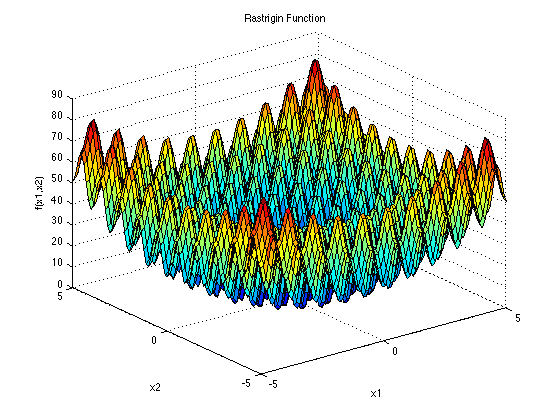
\includegraphics[scale = 0.70]{images/rastring.png}
\caption{Gráfico da função Rastring}
\end{figure}

Nosso objetivo será avaliar e testar todos os parâmetros do Algoritmo Genético para encontrar a função de mínimo para o problema no menor tempo possível, i.e., com a menor quantidade de gerações possível.\\

Foi disponibilizado um código Python a partir da biblioteca geneticalgorithm2 pelo qual iremos nos basear para realizar os testes.


\newpage
\section{Entendendo o Código}
%\begin{lstlisting}[style=python]
%\end{lstlisting} \\

\subsection{Função do problema}
\begin{lstlisting}[style=python]
def f(X):
    dim = len(X)
    OF = 0
    for i in range(dim):
        OF += (X[i]**2) - 10 * math.cos(2 * math.pi * X[i]) + 10
    return OF
\end{lstlisting}

A função $f$ define a função de Rastring, que é a função utilizada para testar aalgoritmos de otimização. A função é avaliada por um vetor de entrada X que é passado como parâmetro.\\

\subsection{Limites do Espaço de Busca}

\begin{lstlisting}[style=python]
varbound = np.array([[-5.12, 5.12]] * 2)
\end{lstlisting}

Aqui é definido os limites do espaço de busca para cada variável que será utilizada na função. É assumido que a função é de 2 dimensões e cada variável pode variar entre $-5.12$ e $5.12$. \\

\subsection{Parâmetros do Algoritmo Genético}

\begin{lstlisting}[style=python]
max_num_iteration = 10  # numero de geracoes
population_size = 10
mutation_probability = 0.001
elit_ratio = 0.2  # percentual de individuos preservados na proxima geracao
crossover_probability = 0.6
parents_portion = 0.8  # proporcao de pais na populacao
crossover_type = 'one_point'
selection_type = 'roulette'
num_experimentos = 5  # numero de rodadas sucessivas

algorithm_param = {
    'max_num_iteration': max_num_iteration,
    'population_size': population_size,
    'mutation_probability': mutation_probability,
    'elit_ratio': elit_ratio,
    'crossover_probability': crossover_probability,
    'parents_portion': parents_portion,
    'crossover_type': crossover_type,
    'max_iteration_without_improv': None,
    'mutation_type': 'uniform_by_center',
    'selection_type': selection_type
}
\end{lstlisting}
Aqui são definidos os parâmetros do GA, como o número máximo de iterações (gerações), tamanho da população, probabilidade de mutação, proporção de elitismo, probabilidade de crossover, tipo de crossover e seleção.\\

\subsection{Inicialização do Modelo}
\begin{lstlisting}[style=python]
model = ga(
    function=f(X=[1, 2, 3]),
    dimension=2,
    variable_type='real',
    variable_boundaries=varbound,
    algorithm_parameters=algorithm_param
)
\end{lstlisting}
Neste trecho é inicializado o modelo do Algoritmo Genético usando a biblioteca \textbf{`geneticalgorithm2`}. A função a ser otimizada é passada junto com a dimensão do problema, tipo de variável, limites das variáveis e parâmetros do algoritmo.\\

\subsection{Execução de Experimentos}

\begin{lstlisting}[style=python]
simulacoes = []
for simu in range(num_experimentos):
    print()
    print('-----------------------------------------------')
    print('Experimento numero = ', simu)
    model.run(
        no_plot=False,
        disable_progress_bar=False,
        set_function=None,
        apply_function_to_parents=False,
        start_generation={'variables': None, 'scores': None},
        studEA=True,
        mutation_indexes=None,
        init_creator=None,
        init_oppositors=None,
        duplicates_oppositor=None,
        remove_duplicates_generation_step=2,
        revolution_oppositor=None,
        revolution_after_stagnation_step=None,
        revolution_part=0,
        population_initializer=Population_initializer(
            select_best_of=1,
            local_optimization_step='never',
            local_optimizer=None
        ),
        stop_when_reached=None,
        callbacks=[
            Callbacks.SavePopulation('callback_pop_example', save_gen_step=1, file_prefix='constraints'),
            Callbacks.PlotOptimizationProcess('callback_plot_example', save_gen_step=300, show=False, main_color='red', file_prefix='plot')
        ],
        middle_callbacks=[],
        time_limit_secs=None,
        save_last_generation_as=None,
        seed=None
    )

    model.plot_generation_scores()
    convergence = model.report
    print("melhores individuos por geracao", convergence)
    simulacoes.append(convergence)
\end{lstlisting}

Aqui, o código executa vários experimentos do GA (definido por \textbf{num\_experimentos}). Em cada experimento, o GA é executado com os parâmetros definidos e o progresso é exibido e plotado. Os resultados de cada geração são armazenados em simulacoes. \\

\subsubsection{Parâmetros do model.run()} 

\begin{enumerate}
    \item \textbf{no\_plot (bool)}:
    \begin{itemize}
        \item Determina se os gráficos de resultados devem ser gerados ou não.
    \end{itemize}
    \item \textbf{disable\_progress\_bar (bool)}:
    \begin{itemize}
        \item Determina se a barra de progresso deve ser desativada.
    \end{itemize}
    \item \textbf{set\_function (callable)}:
    \begin{itemize}
        \item Uma função personalizada que pode ser chamada durante a execução do algoritmo.
        \item Se uma função for fornecida, ela será executada em pontos específicos do algoritmo. Normalmente usada para customizações adicionais.
    \end{itemize}
    \item \textbf{apply\_function\_to\_parents (bool)}:
    \begin{itemize}
        \item Determina se a função set\_function deve ser aplicada aos pais durante a seleção.
    \end{itemize}
    \item \textbf{start\_generation (dict}):
    \begin{itemize}
        \item Um dicionário que define a geração inicial do algoritmo.
        \item Chaves: 
        \begin{itemize}
            \item \textbf{'variables'}: Variáveis iniciais da população.
            \item \textbf{'scores'}: Pontuações iniciais da população.
            \item \textbf{Valor Padrão}: \{'variables': None, 'scores': None\}
        \end{itemize}
    \end{itemize}
    \item \textbf{studEA (bool)}:
    \begin{itemize}
        \item Se o algoritmo deve usar a estratégia de "Estudante" (StudGA).
        \item Se definido como True, o algoritmo usará a estratégia StudGA, que preserva os melhores indivíduos em cada geração.
    \end{itemize}
    \item \textbf{mutation\_indexes (list)}:
    \begin{itemize}
        \item Índices específicos de genes a serem mutados.
    \end{itemize}
    \item \textbf{init\_creator (callable)}:
    \begin{itemize}
        \item Função personalizada para criar a população inicial.
    \end{itemize}
    \item \textbf{init\_oppositors (callable)}:
    \begin{itemize}
        \item Função para criar indivíduos opostos na população inicial.
    \end{itemize}
    \item \textbf{duplicates\_oppositor (callable)}:
    \begin{itemize}
        \item Função para criar indivíduos opostos de duplicados na população.
    \end{itemize}
    \item \textbf{remove\_duplicates\_generation\_step (int)}:
    \begin{itemize}
        \item Passo de geração para remover duplicados.
    \end{itemize}
    \item \textbf{revolution\_oppositor (callable)}:
    \begin{itemize}
        \item Função para criar indivíduos opostos durante a revolução.
    \end{itemize}
    \item \textbf{revolution\_after\_stagnation\_step (int)}:
    \begin{itemize}
        \item Passo de estagnação após o qual a revolução é iniciada.
    \end{itemize}
    \item \textbf{revolution\_part (float)}:
    \begin{itemize}
        \item Proporção da população a ser revolucionada.
    \end{itemize}
    \item \textbf{population\_initializer}:
    \begin{itemize}
        \item Inicializador da população com opções específicas.
        \item Parâmetros:
        \begin{itemize}
            \item \textbf{select\_best\_of}: Seleciona os melhores indivíduos.
            \item \textbf{local\_optimization\_step}: Passo de otimização local.
            \item \textbf{local\_optimizer}: Otimizador local.
        \end{itemize}
    \end{itemize}
    \item \textbf{stop\_when\_reached (float)}:
    \begin{itemize}
        \item Valor da função de aptidão que, se alcançado, interrompe o algoritmo.
    \end{itemize}
    \item \textbf{callbacks (list)}:
    \begin{itemize}
        \item Lista de funções de callback para serem executadas em pontos específicos.

    \end{itemize}
    \item \textbf{middle\_callbacks (list)}:
    \begin{itemize}
        \item Lista de funções de callback intermediárias.
    \end{itemize}
    \item \textbf{time\_limit\_secs (int)}:
    \begin{itemize}
        \item Tempo limite para a execução do algoritmo em segundos.
    \end{itemize}
    \item \textbf{save\_last\_generation\_as (str)}:
    \begin{itemize}
        \item Caminho para salvar a última geração.
    \end{itemize}
    \item \textbf{seed (int)}:
    \begin{itemize}
        \item Semente para o gerador de números aleatórios.
    \end{itemize}
\end{enumerate}




\subsection{Para Análise dos Resultados}
\begin{lstlisting}[style=python]
mean_simulation = []

for i in range(max_num_iteration):
    soma_sim_geracao = 0
    for j in range(num_experimentos):
        soma_sim_geracao += simulacoes[j][i]
    mean_simulation.append(soma_sim_geracao / num_experimentos)

print('----------------------------------------------')
print('Valores medios dos melhores por Geracao')
print(mean_simulation)

fig1, ax1 = plt.subplots()
ax1.set_title('Media dos Melhores por Geracao')
ax1.boxplot(mean_simulation)
plt.show()

plt.plot(mean_simulation, label='Media dos Melhores por Geracao')
plt.legend(loc='upper right')
plt.show()

\end{lstlisting} 

Por fim, o código calcula a média dos melhores indivíduos por geração ao longo dos experimentos e plota esses resultados. Isso ajuda a visualizar a convergência do algoritmo.\\


%\section{Ajustando Algumas Configurações no Código}
\section{Realizando os Experimetos}

\subsection{Ajustando Algumas Configurações no Código}

Antes de iniciar os experimentos, optamos por reorganizar a estrutura do projeto para seguir um padrão de orientação a objetos (POO) com a adesão ao padrão Domain-Driven Design (DDD), tornando-o mais prático para possíveis alterações. 

\begin{figure}[H]
\centering
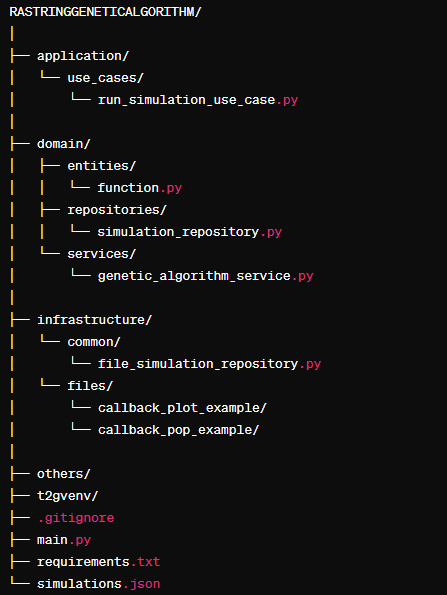
\includegraphics[scale = 0.95]{images/estrutura.png}
\caption{Estrutura do projeto com padrão DDD}
\end{figure}

\begin{itemize}
    \item \textbf{Entidades de Objetos de Valor}: definimos a função de Rastring e os parâmetros do GA como objetos.
    \item \textbf{Serviços}: execução do Algoritmo Genético.
    \item \textbf{Repositórios}: para gerenciar a execução e os resultados das simulações.
    \item \textbf{Interfaces e Implementações}: Implementamos interfaces para as diferentes estratégias do GA (crossover, seleção etc).
\end{itemize}

\subsubsection{main.py}
Neste caso, a \textbf{main.py} ficou com uma estrutura mais amigável e podemos transitar com mais facilidade pelas execuções dos testes e experimentos.\\
%\begin{lstlisting}[style=python]
%\end{lstlisting} \\

Projetamos a função "GeneticAlgorithm" na main.py para tornar mais flexível, executando experimentos e variando um parâmetro específico do Algoritmo Genético para análise dos resultados.\\

\begin{lstlisting}[style=python]
def GeneticAlgorithm(param_name: str, list_of_params: list,
                    dimensions: int,
                    num_of_experiments: int,
                    base_algorithm_params: dict, function,
                    simulation_repo):
    results = {}
    varbound = np.array([[-5.12, 5.12]] * dimensions)

    for param in list_of_params:
        algorithm_params = base_algorithm_params.copy()
        algorithm_params[param_name] = param

        genetic_algorithm_service = GeneticAlgorithmService(
            function,
            dimensions, varbound,
            algorithm_params)

        run_simulation_use_case = RunSimulationUseCase(
            genetic_algorithm_service, simulation_repo)

        simulacoes = run_simulation_use_case.execute(num_of_experiments)

        # Analisando os resultados
        max_iterations = algorithm_params['max_num_iteration']
        mean_simulation = [0] * max_iterations

        for i in range(max_iterations):
            soma_sim_geracao = 0
            for j in range(num_of_experiments):
                if i < len(simulacoes[j]):
                    soma_sim_geracao += simulacoes[j][i]
            mean_simulation[i] = soma_sim_geracao / num_of_experiments

        results[param] = mean_simulation
        print(
            f'{param_name}: {param}, Media dos Melhores por Geracao: {mean_simulation}')

    # Criando a Tabela de Resultados
    max_iterations = max(
        [base_algorithm_params['max_num_iteration']] + [len(r) for r in results.values()])
    data = {
        'Geracao': list(range(1, max_iterations + 1))
    }
    for param in list_of_params:
        mean_simulation = results[param]
        if len(mean_simulation) < max_iterations:
            mean_simulation += [None] * (max_iterations - len(mean_simulation))
        data[f'{param_name} {param}'] = mean_simulation

    df = pd.DataFrame(data)
    print(df)

    # Plotando os resultados
    fig1, ax1 = plt.subplots()
    for param, mean_simulation in results.items():
        ax1.plot(mean_simulation, label=f'{param_name} {param}')
    ax1.set_title('Media dos Melhores por Geracao')
    ax1.set_xlabel('Geracao')
    ax1.set_ylabel('Valor da Funcao')
    ax1.legend()
    plt.show()
\end{lstlisting} \\

\textbf{Parâmetros da Função}\\

\begin{itemize}
    \item \textbf{param\_name (str)}: Nome do parâmetro que será variado (por exemplo, max\_num\_iteration ou mutation\_probability).
    \item \textbf{list\_of\_params (list)}: Lista dos valores que o parâmetro especificado (param\_name) assumirá em diferentes execuções.
    \item \textbf{dimensions (int)}: Dimensão do problema (número de variáveis de decisão no GA).
    \item \textbf{num\_of\_experiments (int)}: Número de experimentos a serem realizados para cada valor do parâmetro.
    \item \textbf{base\_algorithm\_params (dict)}: Dicionário contendo os parâmetros base do GA.
    \item \textbf{function}: Função objetivo a ser minimizada (neste caso, a função de Rastrigin).
    \item \textbf{simulation\_repo}: Repositório para salvar e carregar simulações (instância de FileSimulationRepository).
\end{itemize}



Então, alternamos com mais facilidade cada parâmetro de \textbf{algotithm\_params}, passando para uma lista que, por sua vez, pode ser passada como parâmetro da função que criamos. A imagem abaixo mostra um exemplo, onde estamos alternando \textbf{max\_num\_iteration}, criando uma lista com 10, 20 e 50 iterações que serão consideradas em cada experimento, enquanto os outros parâmetros se mantém fixos no dicionário.

\begin{figure}[H]
\centering
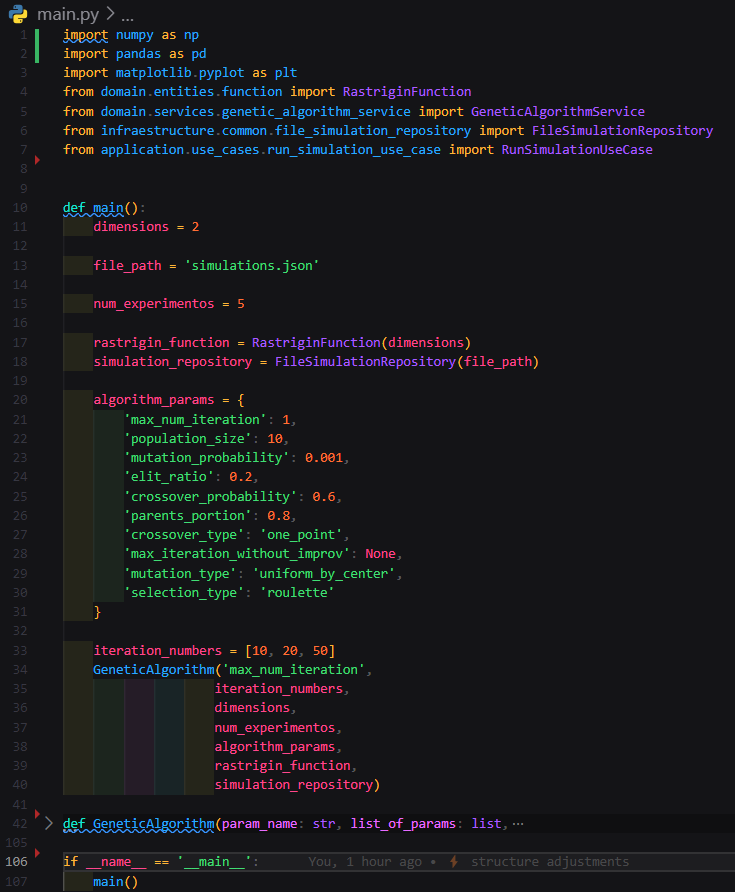
\includegraphics[scale = 0.95]{images/main.png}
\caption{main.py}
\end{figure}

O código completo do projeto atualizado foi inserido em um \href{https://github.com/palomaflsette/RastringGeneticAlgorithm}{repositório do Github}.

\subsection{Experimentos}

Alteramos o código para realizar 2 experimentos para cada parâmetro da lista passado.\\

Por exemplo, se passarmos $iteration\_numbers = [5, 10, 20]$, para cada valor máximo de iteração contido na lista realizaremos 2 experimentos.

\subsubsection{Alternando o número máximo de iterações (max\_num\_iteration)}

Para o número de iterações, foram feitos experimentos considerando 5, 10 e 20.\\

\begin{itemize}
    \item \textbf{Iterações: 5}:
    \begin{itemize}
        \item Experimento 1:
            \begin{figure}[H]
                \centering
                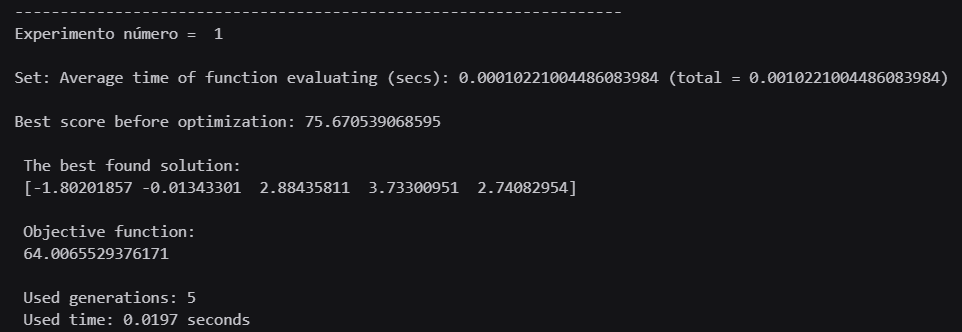
\includegraphics[scale = 0.75]{images/iter5_exp1.png}
                \caption{5 iterações - Experimento 1 }
            \end{figure}

            \begin{figure}[H]
                \centering
                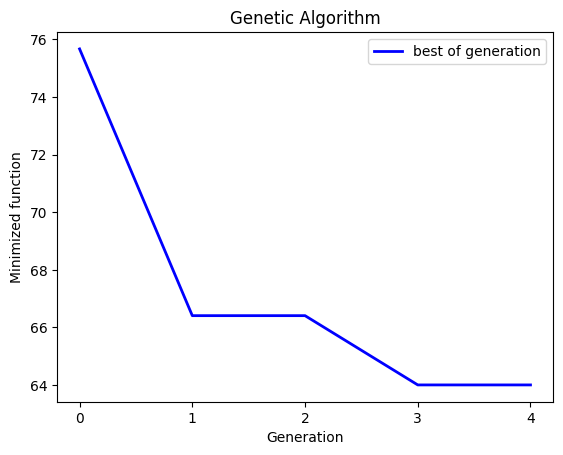
\includegraphics[scale = 0.75]{images/iter5_exp1_graphGA.png}
                \caption{Gráfico GA (5 iterações - Experimento 1) }
            \end{figure}

            \begin{figure}[H]
                \centering
                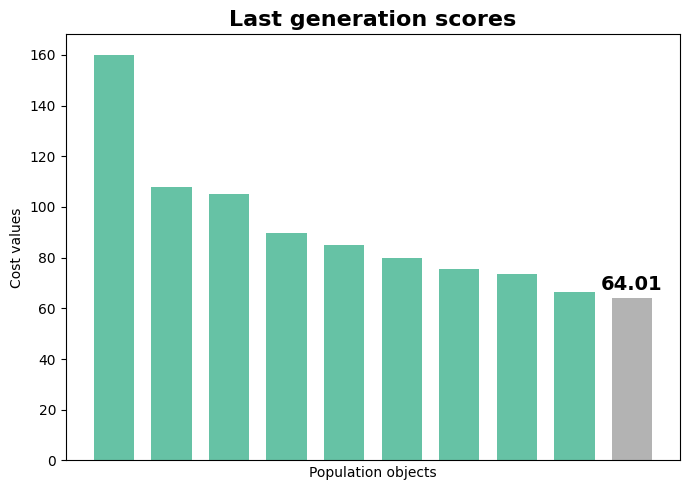
\includegraphics[scale = 0.75]{images/iter5_exp1_graphScore.png}
                \caption{Last Generation Scores (5 iterações - Experimento 1) }
            \end{figure}

            melhores indivíduos por geração:\\
            
            [75.670539068595, \\66.41119417049038,\\ 66.41119417049038,\\ 64.0065529376171,\\ 64.0065529376171]

        \newpage
        \item Experimento 2:
             \begin{figure}[H]
                \centering
                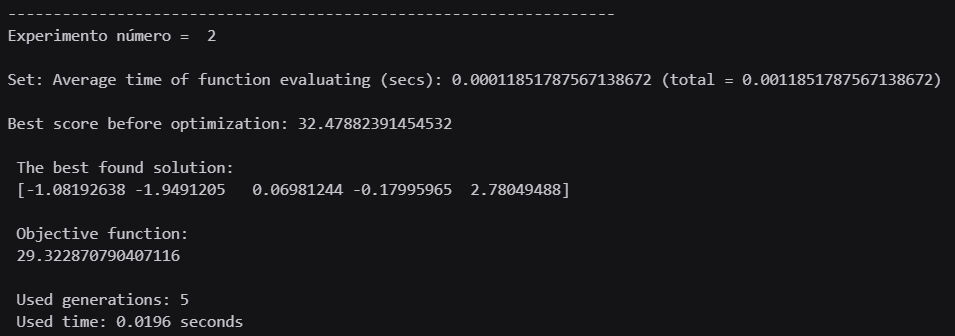
\includegraphics[scale = 0.75]{images/iter5_exp2.png}
                \caption{5 iterações - Experimento 2 }
            \end{figure}

            \begin{figure}[H]
                \centering
                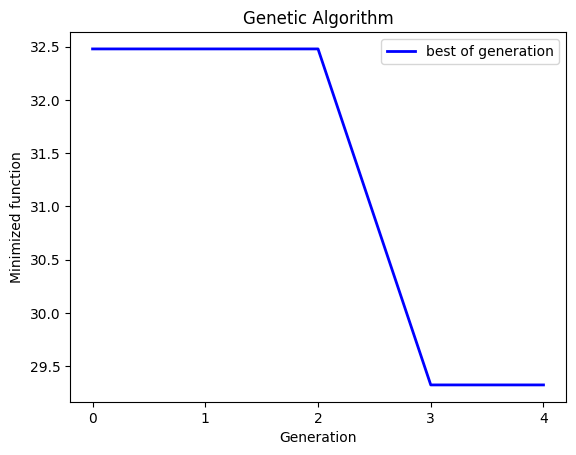
\includegraphics[scale = 0.75]{images/iter5_exp2_graphGA.png}
                \caption{Gráfico GA (5 iterações - Experimento 2) }
            \end{figure}

            \begin{figure}[H]
                \centering
                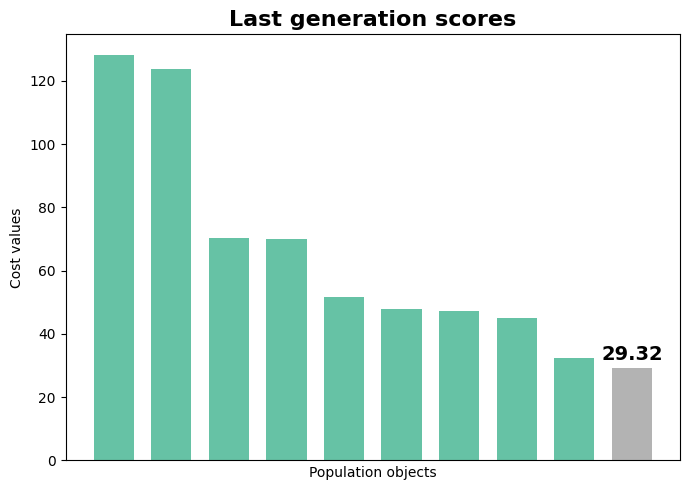
\includegraphics[scale = 0.75]{images/iter5_exp2_graphScore.png}
                \caption{Last Generation Scores (5 iterações - Experimento 2) }
            \end{figure}


            \textbf{melhores indivíduos por geração}: \\
            
            [32.47882391454532,\\ 32.47882391454532,\\ 32.47882391454532,\\ 29.322870790407116,\\ 29.322870790407116] \\

            \textbf{max\_num\_iteration}: 5,\\
            
            \textbf{Média dos Melhores por Geração}:\\
            
            [54.07468149157016,\\ 49.44500904251785,\\ 49.44500904251785,\\ 46.664711864012105,\\ 46.664711864012105]


        
    \end{itemize}
\end{itemize}

\newpage
\begin{itemize}
    \item \textbf{Iterações: 10}:
    \begin{itemize}
        \item Experimento 1:
            \begin{figure}[H]
                \centering
                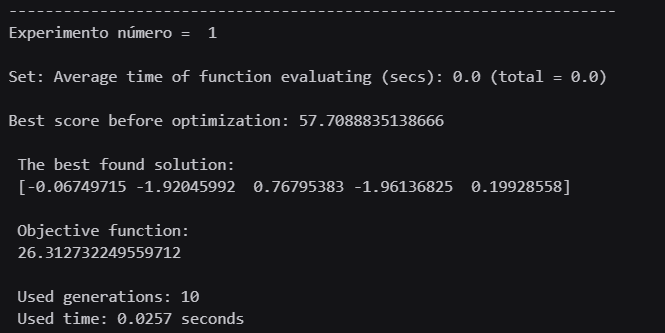
\includegraphics[scale = 0.75]{images/iter10_exp1.png}
                \caption{10 iterações - Experimento 1 }
            \end{figure}

            \begin{figure}[H]
                \centering
                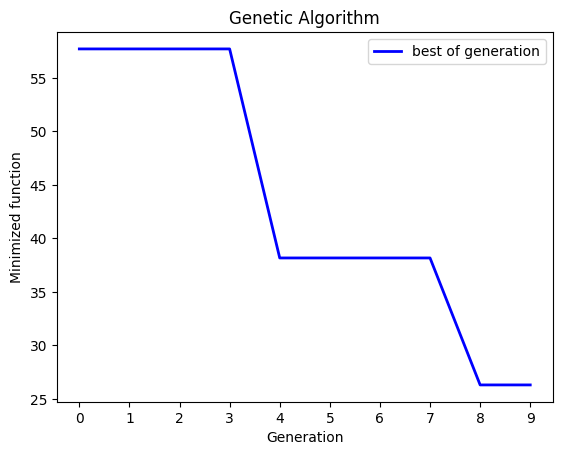
\includegraphics[scale = 0.75]{images/iter10_exp1_graphGA.png}
                \caption{Gráfico GA (10 iterações - Experimento 1) }
            \end{figure}

            \begin{figure}[H]
                \centering
                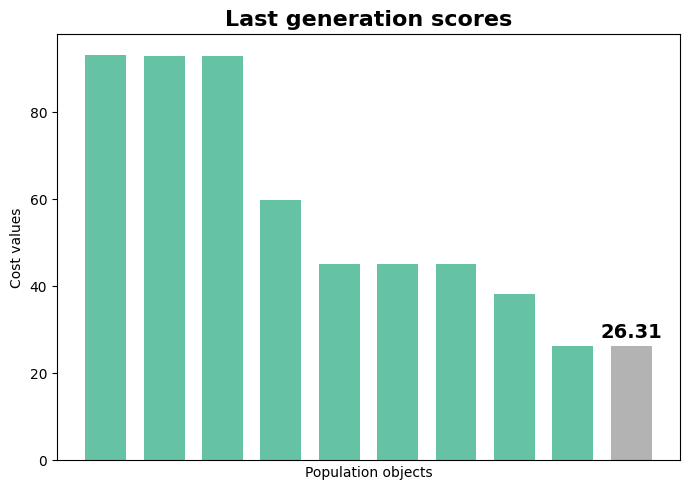
\includegraphics[scale = 0.75]{images/iter10_exp1_graphScore.png}
                \caption{Last Generation Scores (10 iterações - Experimento 1) }
            \end{figure}

            \textbf{Melhores indivíduos por geração}:\\
            
            [57.7088835138666,\\ 57.7088835138666, \\57.7088835138666,\\ 57.7088835138666,\\ 38.17651057673598,\\ 38.17651057673598,\\ 38.17651057673598,\\ 38.17651057673598,\\ 26.312732249559712,\\ 26.312732249559712]

        \newpage
        \item Experimento 2:
             \begin{figure}[H]
                \centering
                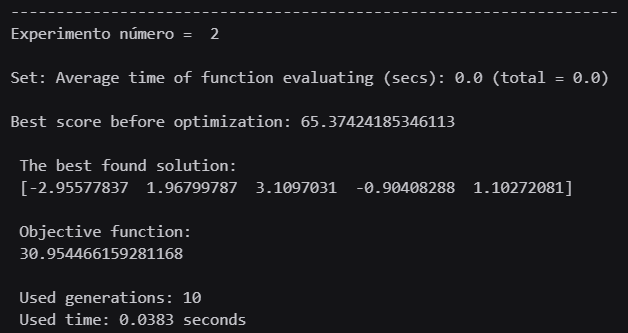
\includegraphics[scale = 0.75]{images/iter10_exp2.png}
                \caption{10 iterações - Experimento 2 }
            \end{figure}

            \begin{figure}[H]
                \centering
                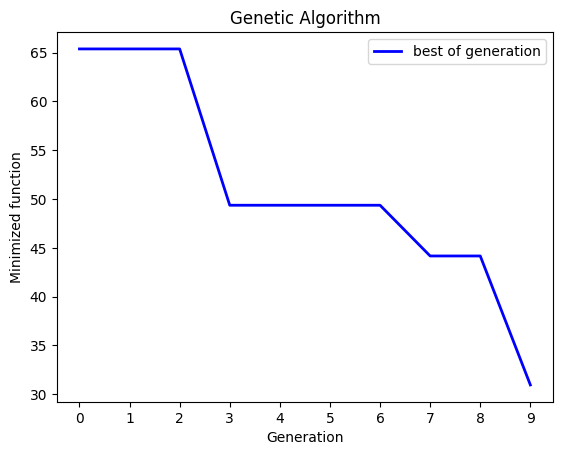
\includegraphics[scale = 0.75]{images/iter10_exp2_graphGA.png}
                \caption{Gráfico GA (10 iterações - Experimento 2) }
            \end{figure}

            \begin{figure}[H]
                \centering
                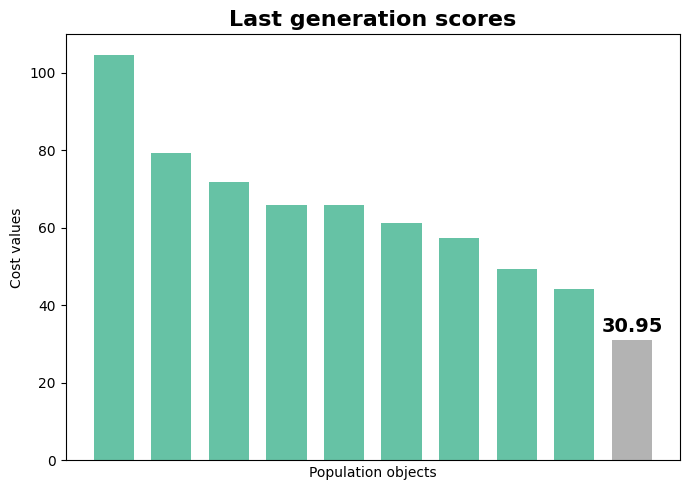
\includegraphics[scale = 0.75]{images/iter10_exp2_graphScore.png}
                \caption{Last Generation Scores (10 iterações - Experimento 2) }
            \end{figure}


            \textbf{melhores indivíduos por geração}: \\
            
            [65.37424185346113,\\ 65.37424185346113,\\ 65.37424185346113,\\ 49.36117809702105,\\ 49.36117809702105,\\ 49.36117809702105,\\ 49.36117809702105,\\ 44.164371284364044,\\ 44.164371284364044,\\ 30.954466159281168] \\

            \textbf{max\_num\_iteration}: 10,\\
            
            \textbf{Média dos Melhores por Geração}:\\
            
            [61.54156268366387,\\ 61.54156268366387,\\ 61.54156268366387,\\ 53.535030805443824,\\ 43.768844336878516,\\ 43.768844336878516,\\ 43.768844336878516,\\ 41.170440930550015,\\ 35.238551766961876,\\ 28.63359920442044]
    \end{itemize}
\end{itemize}

\newpage
\begin{itemize}
    \item \textbf{Iterações: 20}:
    \begin{itemize}
    \item Experimento 1:
            \begin{figure}[H]
                \centering
                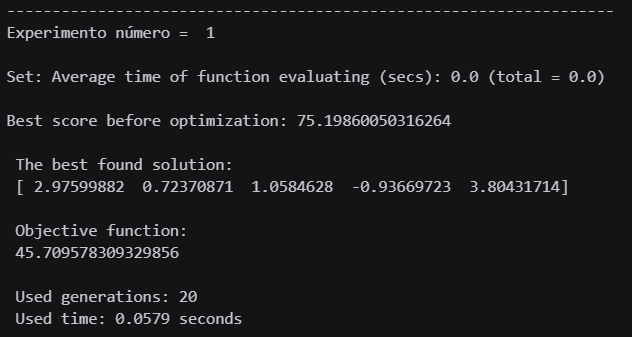
\includegraphics[scale = 0.75]{images/iter20_exp1.png}
                \caption{20 iterações - Experimento 1 }
            \end{figure}

            \begin{figure}[H]
                \centering
                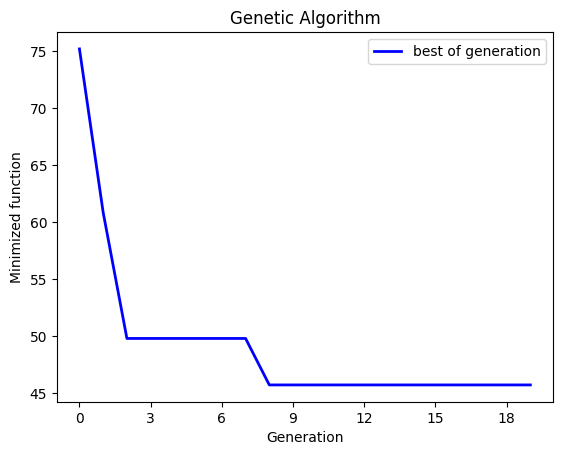
\includegraphics[scale = 0.75]{images/iter20_exp1_graphGA.png}
                \caption{Gráfico GA (20 iterações - Experimento 1) }
            \end{figure}

            \begin{figure}[H]
                \centering
                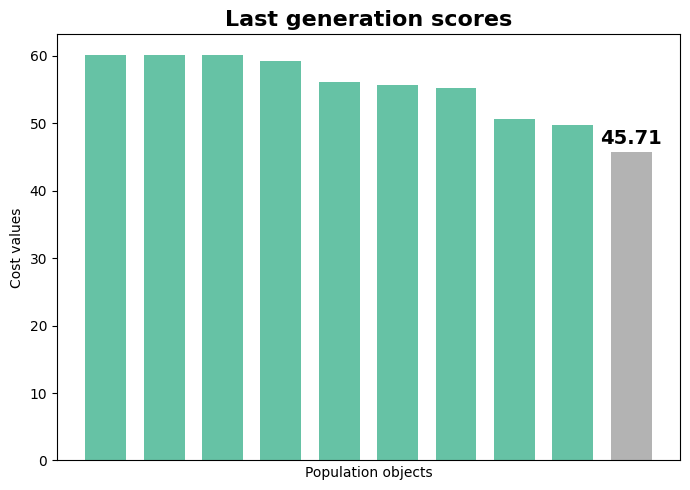
\includegraphics[scale = 0.75]{images/iter20_exp1_graphScore.png}
                \caption{Last Generation Scores (20 iterações - Experimento 1) }
            \end{figure}

            \textbf{Melhores indivíduos por geração}:\\
            
            [75.19860050316264,\\ 60.84020078636968,\\ 49.78817561194869,\\ 49.78817561194869,\\ 49.78817561194869,\\ 49.78817561194869,\\ 49.78817561194869,\\ 49.78817561194869,\\ 45.709578309329856,\\ 45.709578309329856,\\ 45.709578309329856,\\ 45.709578309329856,\\ 45.709578309329856,\\ 45.709578309329856,\\ 45.709578309329856,\\ 45.709578309329856,\\ 45.709578309329856,\\ 45.709578309329856,\\ 45.709578309329856,\\ 45.709578309329856]

        \newpage
        \item Experimento 2:
             \begin{figure}[H]
                \centering
                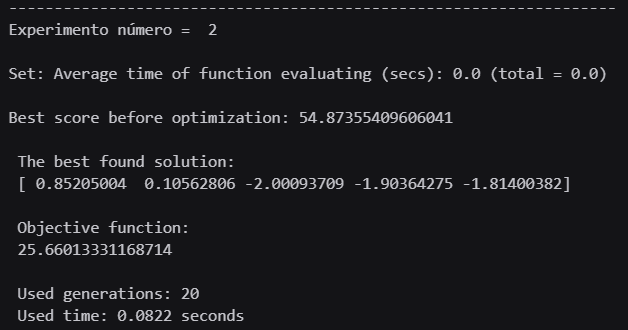
\includegraphics[scale = 0.75]{images/iter20_exp2.png}
                \caption{20 iterações - Experimento 2 }
            \end{figure}

            \begin{figure}[H]
                \centering
                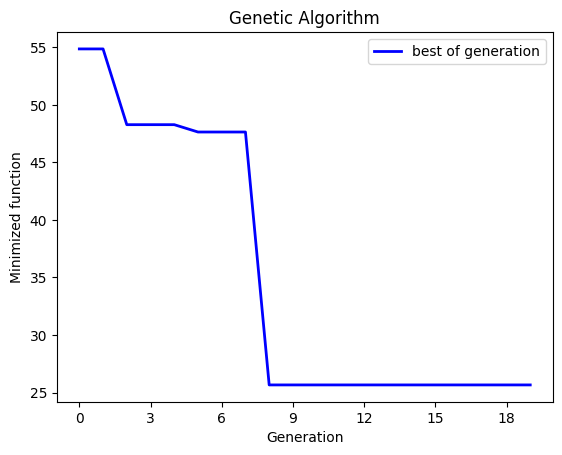
\includegraphics[scale = 0.75]{images/iter20_exp2_graphGA.png}
                \caption{Gráfico GA (20 iterações - Experimento 2) }
            \end{figure}

            \begin{figure}[H]
                \centering
                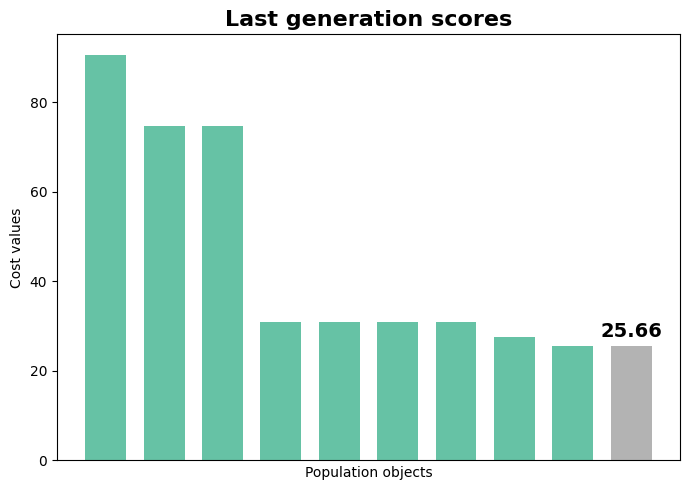
\includegraphics[scale = 0.75]{images/iter20_exp2_graphScore.png}
                \caption{Last Generation Scores (20 iterações - Experimento 2) }
            \end{figure}


            \textbf{melhores indivíduos por geração}: \\
            
            [54.87355409606041,\\ 54.87355409606041,\\ 48.287652570649655,\\ 48.287652570649655,\\ 48.287652570649655,\\ 47.64968702287735,\\ 47.64968702287735,\\ 47.64968702287735,\\ 25.66013331168714,\\ 25.66013331168714,\\ 25.66013331168714,\\ 25.66013331168714,\\ 25.66013331168714,\\ 25.66013331168714,\\ 25.66013331168714,\\ 25.66013331168714,\\ 25.66013331168714,\\ 25.66013331168714,\\ 25.66013331168714, 25.66013331168714] \\

            \textbf{max\_num\_iteration}: 20,\\
            
            \textbf{Média dos Melhores por Geração}:\\
            
            [65.03607729961152,\\ 57.85687744121505,\\ 49.03791409129917,\\ 49.03791409129917,\\ 49.03791409129917,\\ 48.71893131741302,\\ 48.71893131741302,\\ 48.71893131741302,\\ 35.684855810508495,\\ 35.684855810508495,\\ 35.684855810508495,\\ 35.684855810508495,\\ 35.684855810508495,\\ 35.684855810508495,\\ 35.684855810508495,\\ 35.684855810508495,\\ 35.684855810508495,\\ 35.684855810508495,\\ 35.684855810508495,\\ 35.684855810508495]
    \end{itemize}
\end{itemize}

\textbf{Interpretação dos Resultados}:\\

\begin{figure}[H]
    \centering
    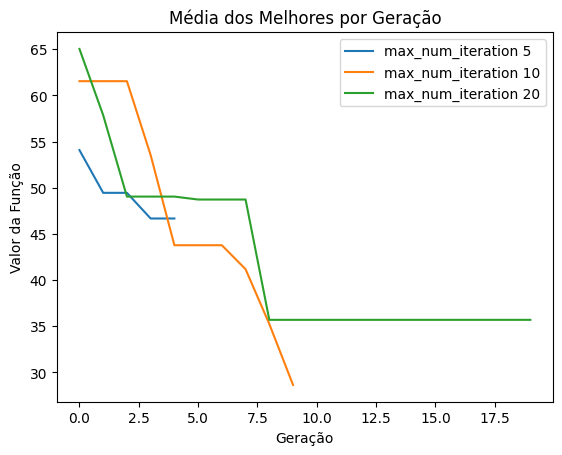
\includegraphics[scale = 0.75]{images/num_iter_graph_media.png}
    \caption{Gráfico comparativo - números de iterações }
\end{figure}

\begin{figure}[H]
    \centering
    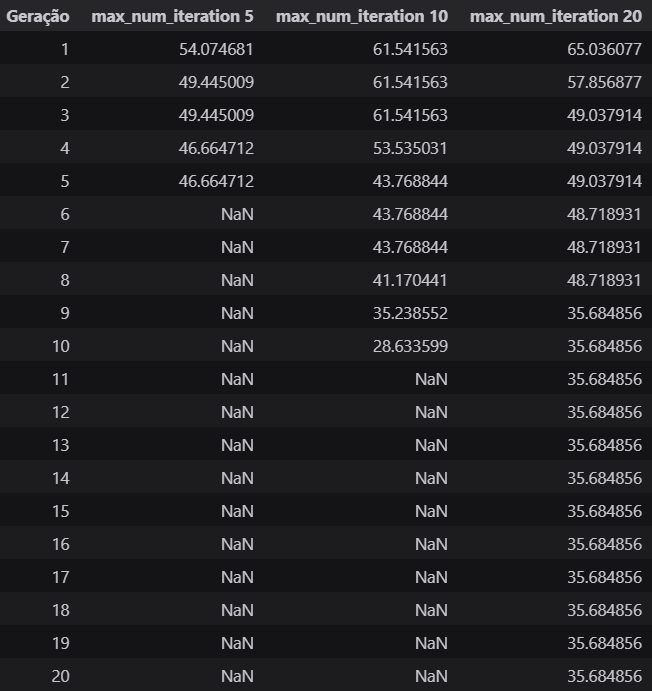
\includegraphics[scale = 0.75]{images/num_iter_tabela_comparativa.png}
    \caption{Tabela comparativa - números de iterações - média dos melhores }
\end{figure}


\begin{enumerate}
    \item \textbf{5 Iterações}:
    \begin{itemize}
        \item O algoritmo mostra uma melhora significativa nas primeiras gerações, mas a convergência parece estagnar rapidamente.
    \end{itemize}
    \item \textbf{10 iterações}:
    \begin{itemize}
        \item O algoritmo continua a melhorar com mais iterações, mostrando uma convergência mais gradual e encontrando soluções melhores do que com apenas 5 iterações.
    \end{itemize}
    \item \textbf{20 Iterações}:
        \begin{itemize}
            \item Com 20 iterações, o algoritmo tem mais tempo para explorar o espaço de soluções e, como resultado, encontra soluções ainda melhores.
            \item As soluções se estabilizam após cerca de 9-10 gerações, indicando uma boa convergência.
        \end{itemize}
\end{enumerate}



Logo, um maior número de iterações permite uma exploração mais aprofundada do espaço de busca, resultando em soluções melhores.\\

A convergência é mais rápida nas primeiras iterações, mas melhorias adicionais requerem mais iterações.\\

Encontrar um equilíbrio entre o número de iterações e o tempo de execução é crucial para um desempenho eficiente do Algoritmo Genético.



\newpage
\subsubsection{Alternando o tamanho da população (population\_size)}

Neste caso, faremos o experimento para tamanhos de população 5 e 20, executando 2 experimentos para cada com um número máximo de 10 iterações.

\begin{itemize}
    \item \textbf{Tamanho da população: 5}:
    \begin{itemize}
        \item Experimento 1:
            \begin{figure}[H]
                \centering
                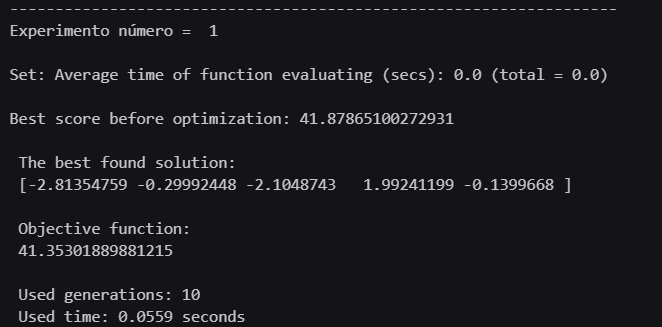
\includegraphics[scale = 0.75]{images/popsize5_exp1.png}
                \caption{5 indivíduos - Experimento 1 }
            \end{figure}

            \begin{figure}[H]
                \centering
                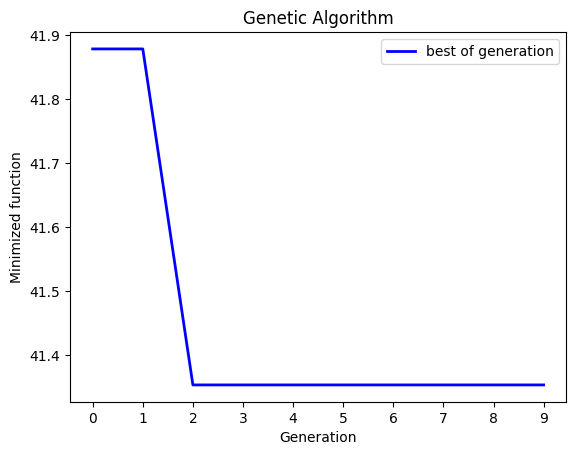
\includegraphics[scale = 0.75]{images/popsize5_exp1_graphGA.png}
                \caption{Gráfico GA (5 indivíduos - Experimento 1) }
            \end{figure}

            \begin{figure}[H]
                \centering
                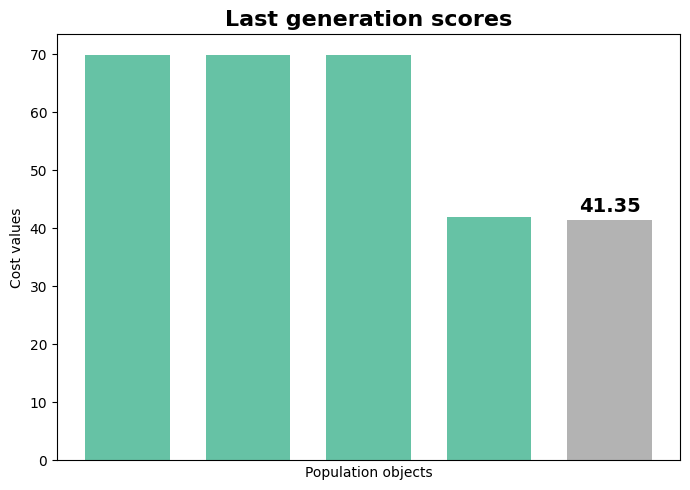
\includegraphics[scale = 0.75]{images/popsize5_exp1_graphScore.png}
                \caption{Last Generation Scores (5 indivíduos - Experimento 1) }
            \end{figure}

            \textbf{Melhores indivíduos por geração}:\\
            
            [41.87865100272931,\\ 41.87865100272931,\\ 41.35301889881215,\\ 41.35301889881215,\\ 41.35301889881215,\\ 41.35301889881215,\\ 41.35301889881215,\\ 41.35301889881215,\\ 41.35301889881215,\\ 41.35301889881215]

        \newpage
        \item Experimento 2:
            \begin{figure}[H]
                \centering
                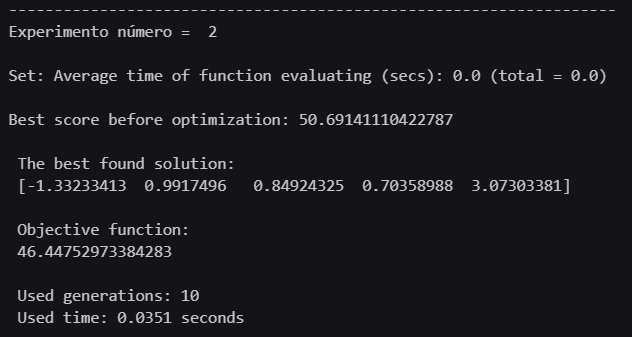
\includegraphics[scale = 0.75]{images/popsize5_exp2.png}
                \caption{5 indivíduos - Experimento 2 }
            \end{figure}

            \begin{figure}[H]
                \centering
                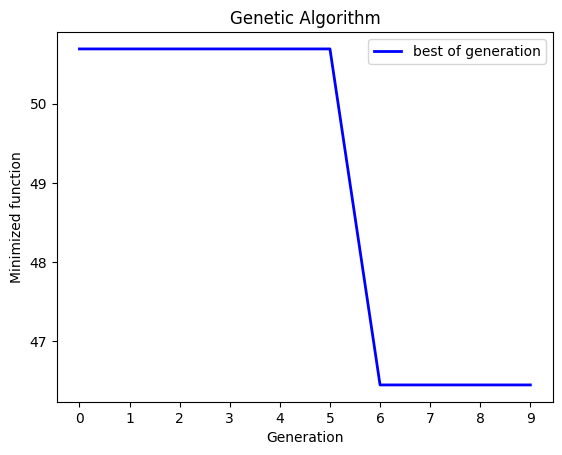
\includegraphics[scale = 0.75]{images/popsize5_exp2_graphGA.png}
                \caption{Gráfico GA (5 indivíduos - Experimento 2) }
            \end{figure}

            \begin{figure}[H]
                \centering
                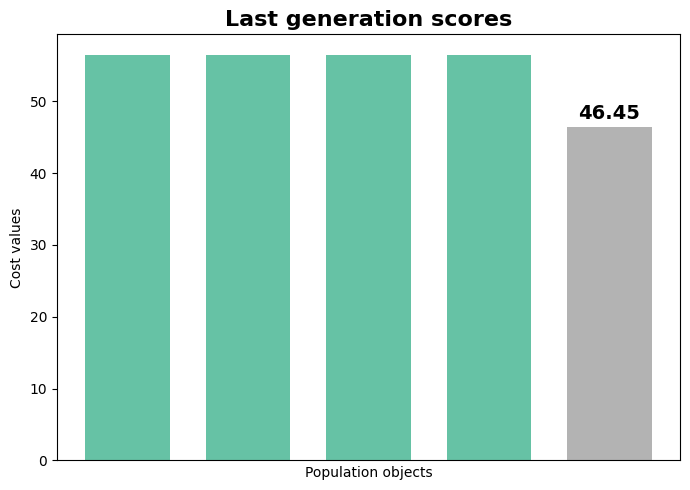
\includegraphics[scale = 0.75]{images/popsize5_exp2_graphScore.png}
                \caption{Last Generation Scores (5 indivíduos - Experimento 2) }
            \end{figure}

            \textbf{Melhores indivíduos por geração}:\\
            
            [50.69141110422787,\\ 50.69141110422787,\\ 50.69141110422787,\\ 50.69141110422787,\\ 50.69141110422787,\\ 50.69141110422787,\\ 46.44752973384283,\\ 46.44752973384283,\\ 46.44752973384283,\\ 46.44752973384283] \\

            \textbf{population\_size}: 5,\\
            
            \textbf{Média dos Melhores por Geração}:\\
            
            [46.28503105347859,\\ 46.28503105347859,\\ 46.02221500152001,\\ 46.02221500152001,\\ 46.02221500152001,\\ 46.02221500152001,\\ 43.90027431632749,\\ 43.90027431632749,\\ 43.90027431632749,\\ 43.90027431632749]
    \end{itemize}
\end{itemize}

\newpage
\begin{itemize}
    \item \textbf{Tamanho da população: 20}:
    \begin{itemize}
        \item Experimento 1:
            \begin{figure}[H]
                \centering
                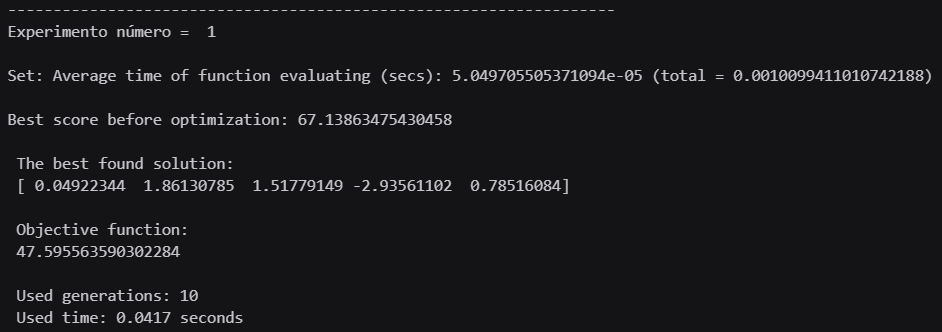
\includegraphics[scale = 0.75]{images/popsize20_exp1.png}
                \caption{20 indivíduos - Experimento 1 }
            \end{figure}

            \begin{figure}[H]
                \centering
                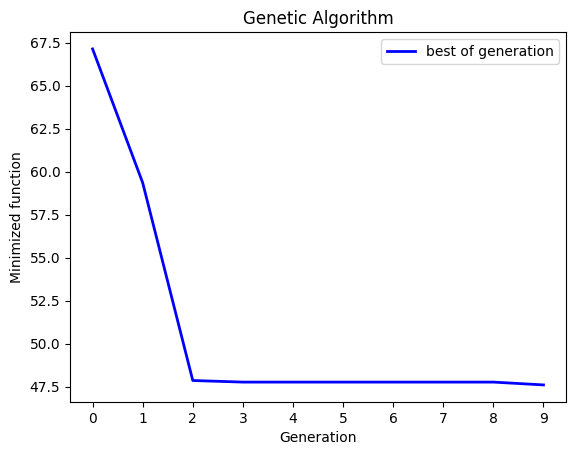
\includegraphics[scale = 0.75]{images/popsize20_exp1_graphGA.png}
                \caption{Gráfico GA (20 indivíduos - Experimento 1) }
            \end{figure}

            \begin{figure}[H]
                \centering
                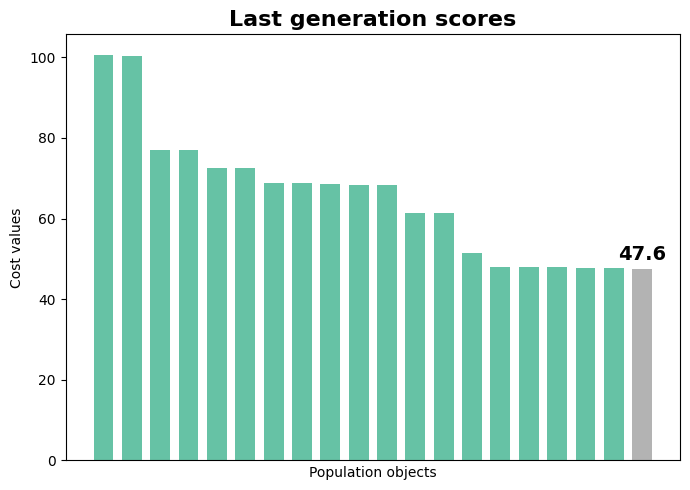
\includegraphics[scale = 0.75]{images/popsize20_exp1_graphScore.png}
                \caption{Last Generation Scores (20 indivíduos - Experimento 1) }
            \end{figure}

            \textbf{Melhores indivíduos por geração}:\\
            
            [67.13863475430458,\\ 59.35607935381861,\\ 47.852257482922,\\ 47.76001325029767,\\ 47.76001325029767,\\ 47.76001325029767,\\ 47.76001325029767,\\ 47.76001325029767,\\ 47.76001325029767,\\ 47.595563590302284]

        \newpage
        \item Experimento 2:
            \begin{figure}[H]
                \centering
                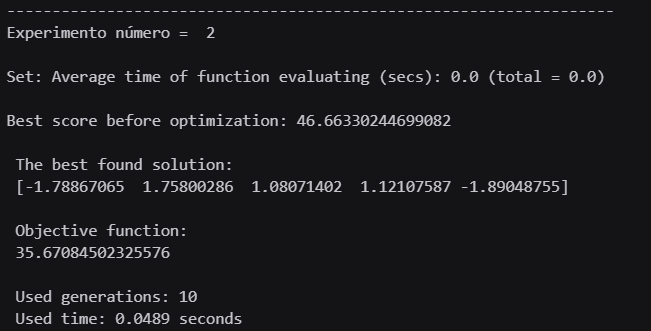
\includegraphics[scale = 0.75]{images/popsize20_exp2.png}
                \caption{20 indivíduos - Experimento 2 }
            \end{figure}

            \begin{figure}[H]
                \centering
                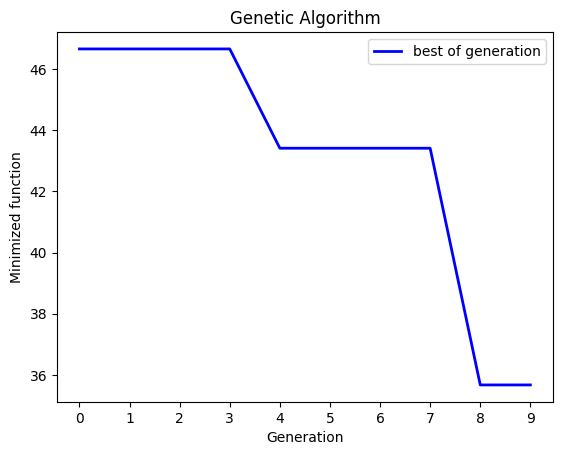
\includegraphics[scale = 0.75]{images/popsize20_exp2_graphGA.png}
                \caption{Gráfico GA (20 indivíduos - Experimento 2) }
            \end{figure}

            \begin{figure}[H]
                \centering
                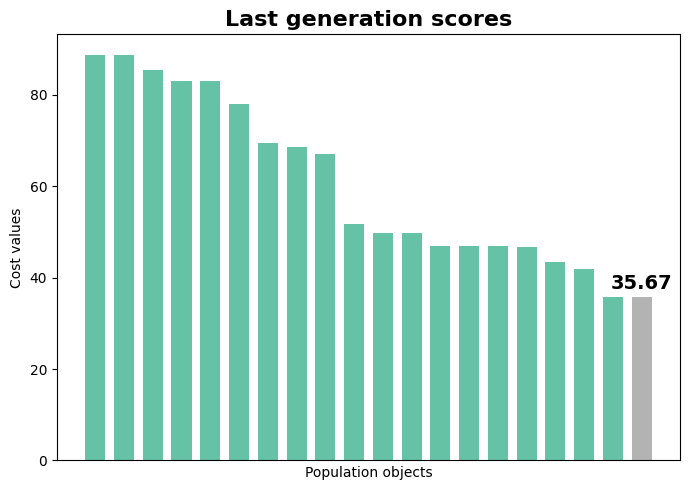
\includegraphics[scale = 0.75]{images/popsize20_exp2_graphScore.png}
                \caption{Last Generation Scores (20 indivíduos - Experimento 2) }
            \end{figure}

            \textbf{Melhores indivíduos por geração}:\\
            
            [46.66330244699082,\\ 46.66330244699082,\\ 46.66330244699082,\\ 46.66330244699082,\\ 43.414645332845886,\\ 43.414645332845886,\\ 43.414645332845886,\\ 43.414645332845886,\\ 35.67084502325576,\\ 35.67084502325576] \\

            \textbf{population\_size}: 20,\\
            
            \textbf{Média dos Melhores por Geração}:\\
            
            [56.9009686006477,\\ 53.00969090040471,\\ 47.25777996495641,\\ 47.21165784864424,\\ 45.58732929157178,\\ 45.58732929157178,\\ 45.58732929157178,\\ 45.58732929157178,\\ 41.71542913677671,\\ 41.63320430677902]
    \end{itemize}
\end{itemize}

\textbf{Interpretação dos Resultados}:\\

\begin{figure}[H]
    \centering
    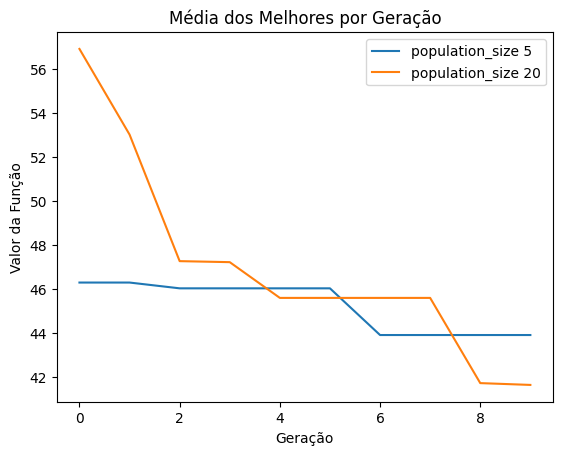
\includegraphics[scale = 0.75]{images/popsize_graph_media.png}
    \caption{Gráfico comparativo - Tamanhos de populções }
\end{figure}

\begin{figure}[H]
    \centering
    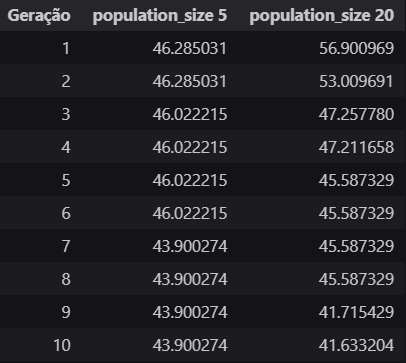
\includegraphics[scale = 0.90]{images/popsize_tabela_comparativa.png}
    \caption{Tabela comparativa - tamanhos de populações - média dos melhores }
\end{figure}


\begin{enumerate}
    \item \textbf{População com 5 indivíduos}:
    \begin{itemize}
        \item A população menor leva a uma menor diversidade genética, o que pode resultar em convergência mais rápida, mas também pode levar a uma convergência prematura.
        \item Observa-se que os valores da função objetivo estabilizam mais rapidamente, mas não alcançam valores tão baixos quanto os obtidos com uma população maior.
        \item O tamanho de população de 5 mostra uma melhoria mais gradual, com menos variabilidade inicial.
    \end{itemize}
    \item \textbf{População com 20 indivíduos}:
    \begin{itemize}
        \item Uma população maior permite uma maior diversidade genética, o que pode ajudar a explorar melhor o espaço de busca.
        \item Embora a convergência seja um pouco mais lenta, os valores finais da função objetivo tendem a ser menores, indicando melhores soluções.
        \item O tamanho de população de 20 mostra uma queda rápida nas primeiras gerações, indicando uma exploração mais eficaz do espaço de soluções.
    \end{itemize}
\end{enumerate}

Logo, \\

Um tamanho maior de população permite uma melhor exploração do espaço de busca e, geralmente, encontra soluções melhores.\\
Uma população menor pode levar a uma convergência mais rápida, mas com maior risco de ficar presa em ótimos locais.\\
Encontrar um equilíbrio entre o tamanho da população e a diversidade genética é crucial para um desempenho eficiente do Algoritmo Genético.










\newpage
\subsubsection{Alternando a probabilidade de mutação (mutation\_probability)}

Neste caso, alternamos os valores de probabilidade de mutação, considerando 0.001 e 0.005, executando 2 experimentos para cada.

\begin{itemize}
    \item \textbf{mutation\_probability = 0.001}:
    \begin{itemize}
        \item Experimento 1:
            \begin{figure}[H]
                \centering
                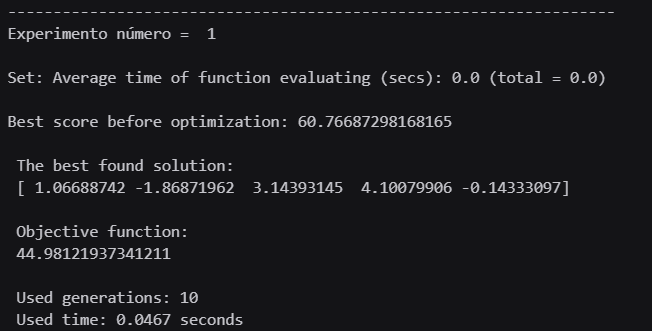
\includegraphics[scale = 0.75]{images/mutprob001_exp1.png}
                \caption{mutation\_probability =0.001 - Experimento 1 }
            \end{figure}

            \begin{figure}[H]
                \centering
                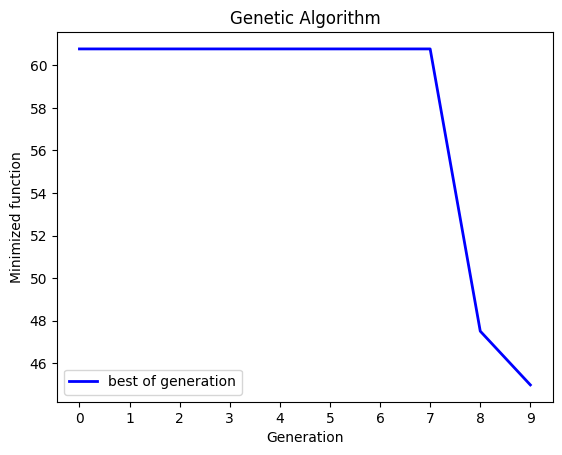
\includegraphics[scale = 0.75]{images/mutprob001_exp1_graphGA.png}
                \caption{Gráfico GA (mutation\_probability =0.001 - Experimento 1) }
            \end{figure}

            \begin{figure}[H]
                \centering
                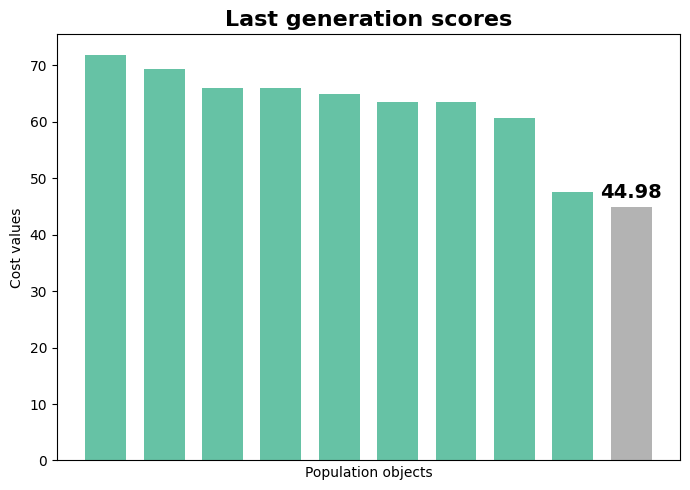
\includegraphics[scale = 0.75]{images/mutprob001_exp1_graphScore.png}
                \caption{Last Generation Scores (mutation\_probability =0.001 - Experimento 1) }
            \end{figure}

            \textbf{Melhores indivíduos por geração}:\\
            
            [60.76687298168165,\\ 60.76687298168165,\\ 60.76687298168165,\\ 60.76687298168165,\\ 60.76687298168165,\\ 60.76687298168165,\\ 60.76687298168165,\\ 60.76687298168165,\\ 47.506909141167775,\\ 44.98121937341211]

        \newpage
        \item Experimento 2:
            \begin{figure}[H]
                \centering
                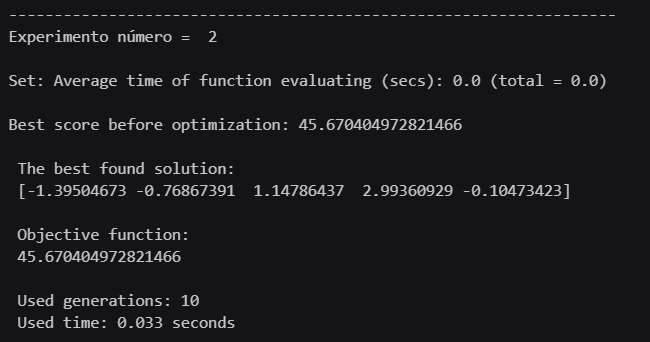
\includegraphics[scale = 0.75]{images/mutprob001_exp2.png}
                \caption{mutation\_probability =0.001 - Experimento 2 }
            \end{figure}

            \begin{figure}[H]
                \centering
                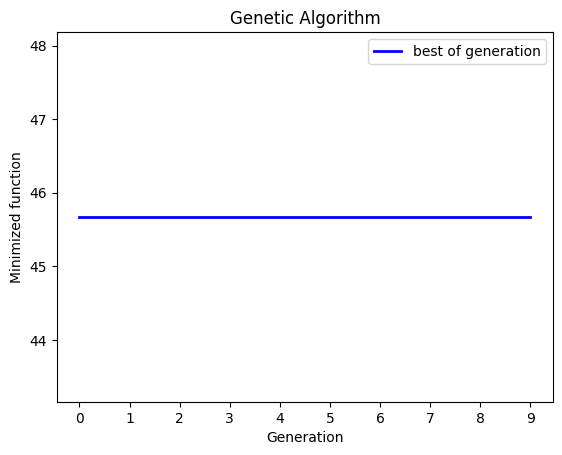
\includegraphics[scale = 0.75]{images/mutprob001_exp2_graphGA.png}
                \caption{Gráfico GA (mutation\_probability =0.001 - Experimento 2) }
            \end{figure}

            \begin{figure}[H]
                \centering
                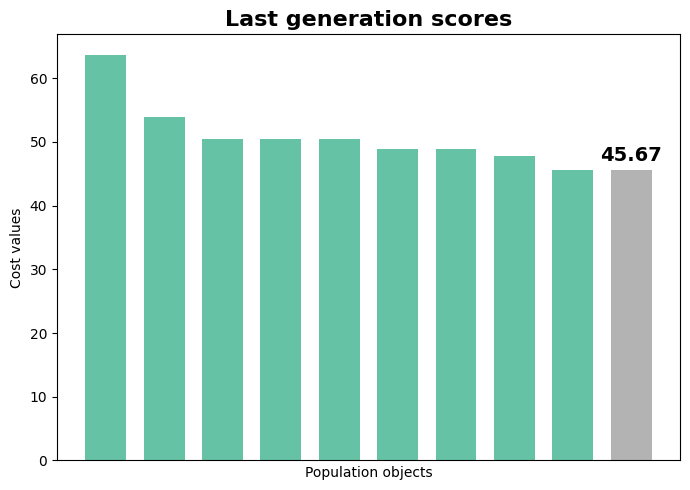
\includegraphics[scale = 0.75]{images/mutprob001_exp2_graphScore.png}
                \caption{Last Generation Scores (mutation\_probability =0.001 - Experimento 2) }
            \end{figure}

            \textbf{Melhores indivíduos por geração}:\\
            
            [45.670404972821466,\\ 45.670404972821466,\\ 45.670404972821466,\\ 45.670404972821466,\\ 45.670404972821466,\\ 45.670404972821466,\\ 45.670404972821466,\\ 45.670404972821466,\\ 45.670404972821466,\\ 45.670404972821466] \\

            \textbf{mutation\_probability}: 0.001,\\
            
            \textbf{Média dos Melhores por Geração}:\\
            
            [53.21863897725156,\\ 53.21863897725156,\\ 53.21863897725156,\\ 53.21863897725156,\\ 53.21863897725156,\\ 53.21863897725156,\\ 53.21863897725156,\\ 53.21863897725156,\\ 46.58865705699462,\\ 45.32581217311679]
    \end{itemize}
\end{itemize}

\newpage
\begin{itemize}
    \item \textbf{mutation\_probability = 0.05}:
    \begin{itemize}
        \item Experimento 1:
            \begin{figure}[H]
                \centering
                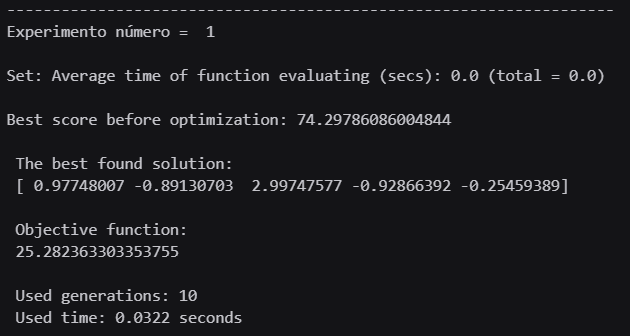
\includegraphics[scale = 0.75]{images/mutprob05_exp1.png}
                \caption{mutation\_probability =0.05 - Experimento 1 }
            \end{figure}

            \begin{figure}[H]
                \centering
                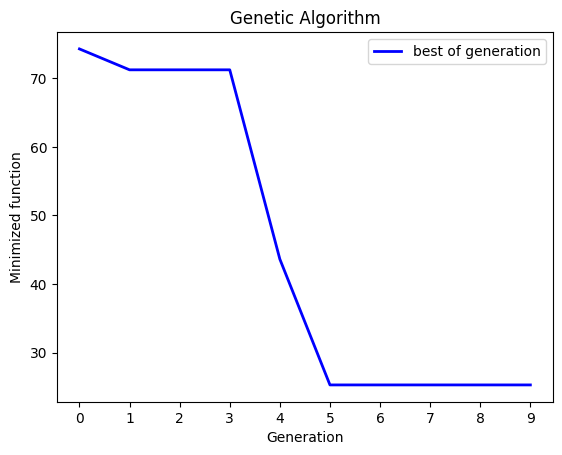
\includegraphics[scale = 0.75]{images/mutprob05_exp1_graphGA.png}
                \caption{Gráfico GA (mutation\_probability =0.05 - Experimento 1) }
            \end{figure}

            \begin{figure}[H]
                \centering
                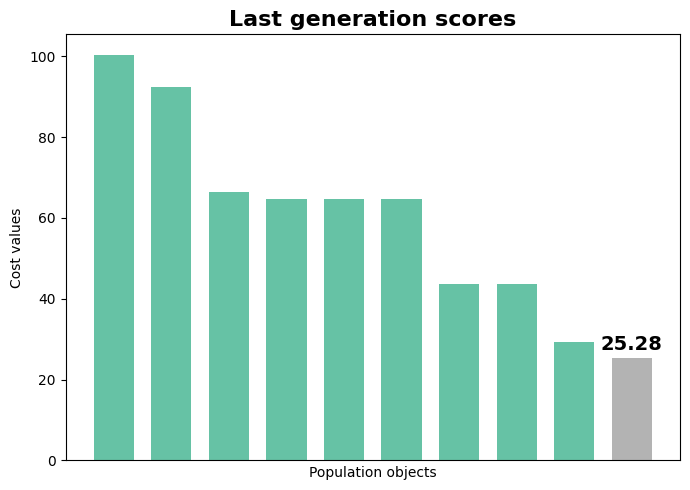
\includegraphics[scale = 0.75]{images/mutprob05_exp1_graphScore.png}
                \caption{Last Generation Scores (mutation\_probability =0.05 - Experimento 1) }
            \end{figure}

            \textbf{Melhores indivíduos por geração}:\\
            
            [74.29786086004844,\\ 71.24896864440962,\\ 71.24896864440962,\\ 71.24896864440962,\\ 43.62959313746951,\\ 25.282363303353755,\\ 25.282363303353755,\\ 25.282363303353755,\\ 25.282363303353755,\\ 25.282363303353755]

        \newpage
        \item Experimento 2:
            \begin{figure}[H]
                \centering
                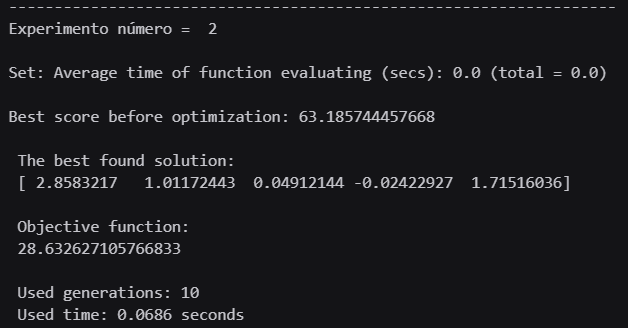
\includegraphics[scale = 0.75]{images/mutprob05_exp2.png}
                \caption{mutation\_probability =0.05 - Experimento 2 }
            \end{figure}

            \begin{figure}[H]
                \centering
                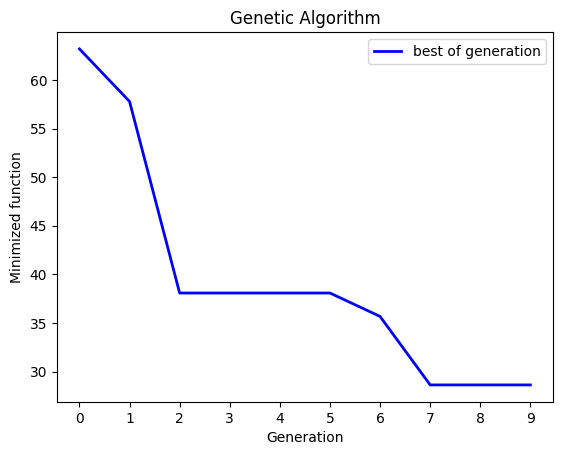
\includegraphics[scale = 0.75]{images/mutprob05_exp2_graphGA.png}
                \caption{Gráfico GA (mutation\_probability =0.05 - Experimento 2) }
            \end{figure}

            \begin{figure}[H]
                \centering
                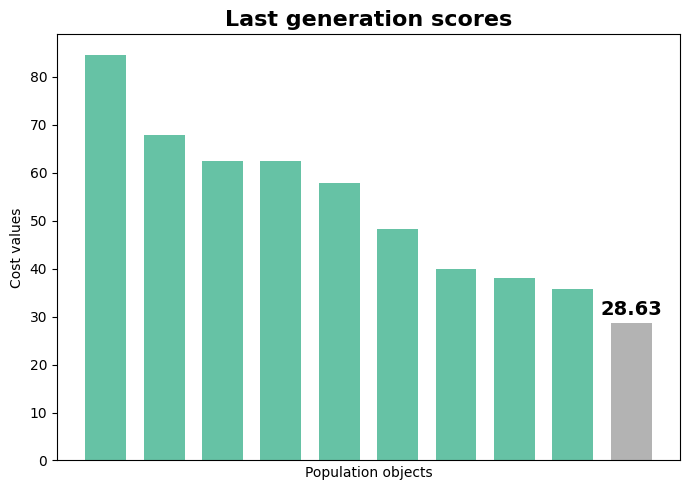
\includegraphics[scale = 0.75]{images/mutprob05_exp2_graphScore.png}
                \caption{Last Generation Scores (mutation\_probability =0.05 - Experimento 2) }
            \end{figure}

            \textbf{Melhores indivíduos por geração}:\\
            
            [63.185744457668,\\ 57.779694559235466,\\ 38.083138166569825,\\ 38.083138166569825,\\ 38.083138166569825,\\ 38.083138166569825,\\ 35.6753383487754,\\ 28.632627105766833,\\ 28.632627105766833,\\ 28.632627105766833] \\

            \textbf{mutation\_probability}: 0.05,\\
            
            \textbf{Média dos Melhores por Geração}:\\
            
            [68.74180265885822,\\ 64.51433160182253,\\ 54.66605340548972,\\ 54.66605340548972,\\ 40.85636565201967,\\ 31.68275073496179,\\ 30.478850826064576,\\ 26.957495204560296,\\ 26.957495204560296,\\ 26.957495204560296]
    \end{itemize}
\end{itemize}



\textbf{Interpretação dos Resultados}:\\

\begin{figure}[H]
    \centering
    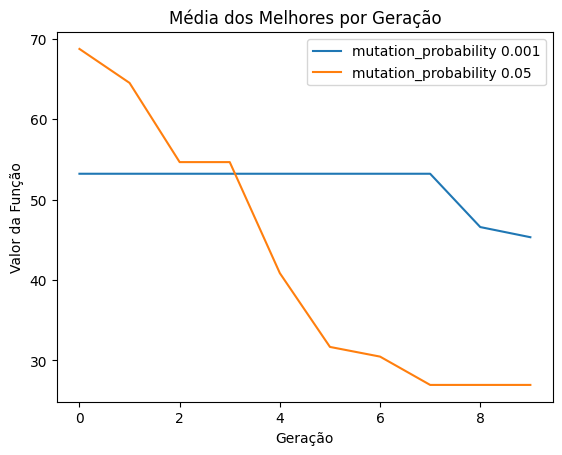
\includegraphics[scale = 0.75]{images/mutprob_graph_media.png}
    \caption{Gráfico comparativo - mutation\_probability }
\end{figure}

\begin{figure}[H]
    \centering
    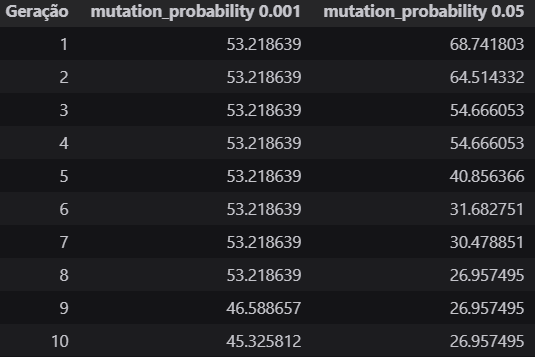
\includegraphics[scale = 0.90]{images/mutprob_tabela_comparativa.png}
    \caption{Tabela comparativa - mutation\_probability - média dos melhores }
\end{figure}



\begin{enumerate}
    \item \textbf{mutation\_probability = 0.001}:
    \begin{itemize}
        \item O gráfico representa uma baixa probabilidade de mutação. A função objetivo começa em torno de 53 e melhora lentamente ao longo das gerações, estabilizando em torno de 45 na 10ª geração.
        \item A baixa probabilidade resulta em menos diversidade, levando a uma melhoria mais lenta.
        \item Adequado para cenários onde a estabilidade é preferida e as soluções razoáveis são aceitáveis.
        \item Convergência lenta, menor diversidade genética.
    \end{itemize}
    \item \textbf{mutation\_probability = 0.05}:
    \begin{itemize}
        \item Representa uma maior probabilidade de mutação.
        \item A função objetivo começa mais alta, em torno de 68, mas melhora significativamente nas primeiras gerações.
        \item A convergência é mais rápida e os valores finais da função objetivo são mais baixos, indicando melhores soluções.
        \item Permite maior diversidade genética, ajudando a explorar melhor o espaço de soluções e evitando a convergência prematura.
        \item Melhor para explorar o espaço de soluções de forma agressiva, encontrando soluções de alta qualidade.
    \end{itemize}
\end{enumerate}









\newpage
\subsubsection{Alternando a taxa de elitismo (elit\_ratio)}

\begin{itemize}
    \item \textbf{elit\_ratio = 0.2}:
    \begin{itemize}
        \item Experimento 1:
            \begin{figure}[H]
                \centering
                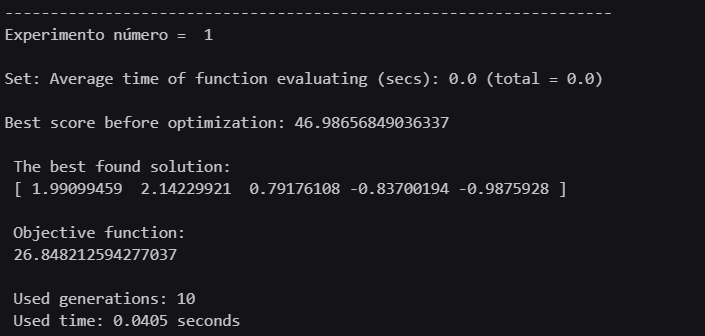
\includegraphics[scale = 0.75]{images/elitratio02_exp1.png}
                \caption{elit\_ratio = 0.2 - Experimento 1 }
            \end{figure}

            \begin{figure}[H]
                \centering
                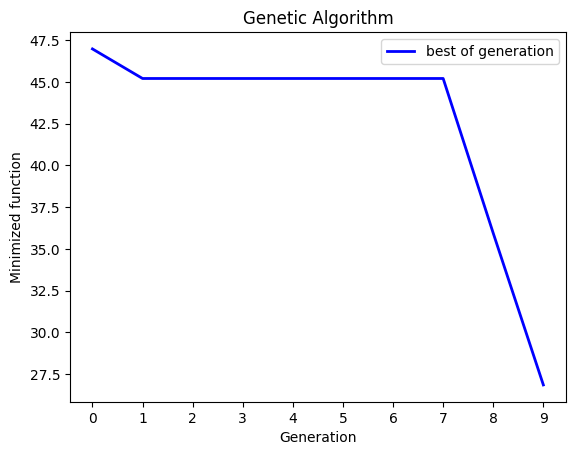
\includegraphics[scale = 0.75]{images/elitratio02_exp1_graphGA.png}
                \caption{Gráfico GA (elit\_ratio = 0.2 - Experimento 1) }
            \end{figure}

            \begin{figure}[H]
                \centering
                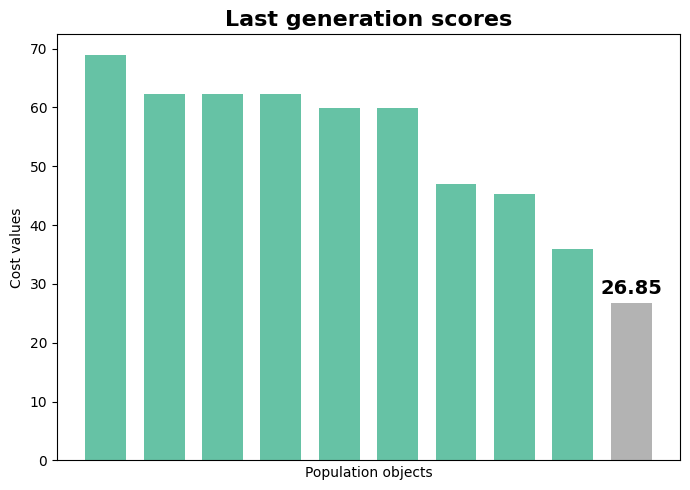
\includegraphics[scale = 0.75]{images/elitratio02_exp1_graphScore.png}
                \caption{Last Generation Scores (elit\_ratio = 0.2 - Experimento 1) }
            \end{figure}

            \textbf{Melhores indivíduos por geração}:\\
            
            [46.98656849036337,\\ 45.21450278577384,\\ 45.21450278577384,\\ 45.21450278577384,\\ 45.21450278577384,\\ 45.21450278577384,\\ 45.21450278577384,\\ 45.21450278577384,\\ 35.93855619484212,\\ 26.848212594277037]

        \newpage
        \item Experimento 2:
            \begin{figure}[H]
                \centering
                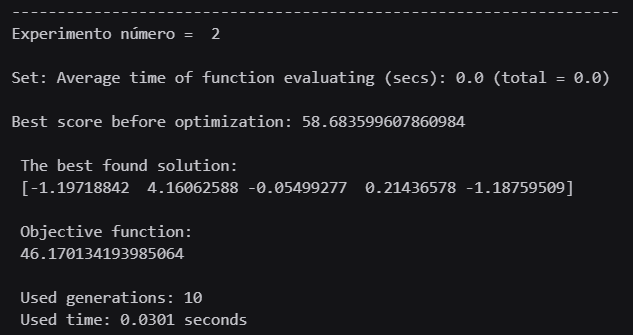
\includegraphics[scale = 0.75]{images/elitratio02_exp2.png}
                \caption{elit\_ratio = 0.2 - Experimento 2 }
            \end{figure}

            \begin{figure}[H]
                \centering
                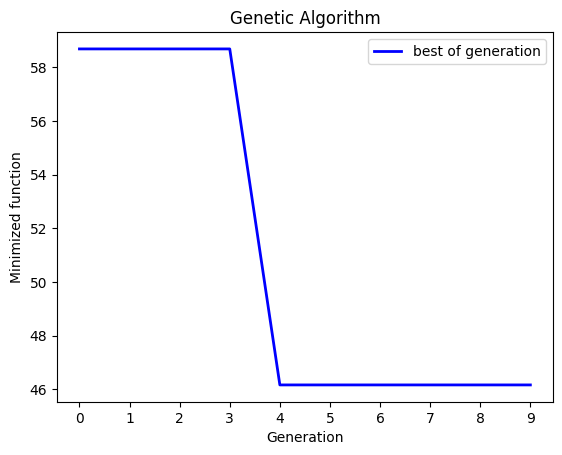
\includegraphics[scale = 0.75]{images/elitratio02_exp2_graphGA.png}
                \caption{Gráfico GA (elit\_ratio = 0.2 - Experimento 2) }
            \end{figure}

            \begin{figure}[H]
                \centering
                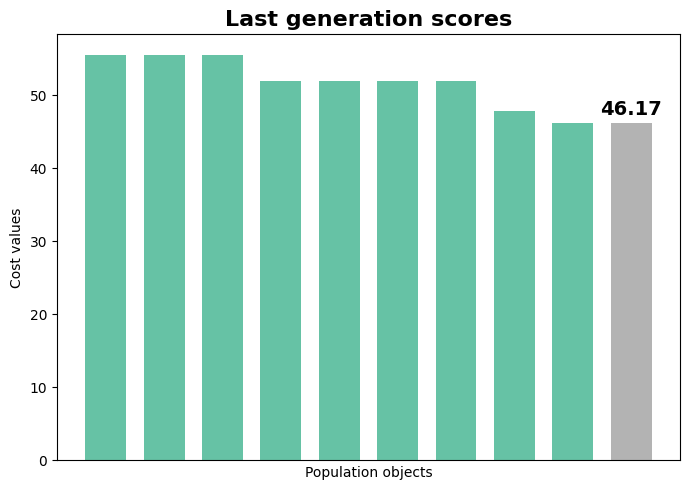
\includegraphics[scale = 0.75]{images/elitratio02_exp2_graphScore.png}
                \caption{Last Generation Scores (elit\_ratio = 0.2 - Experimento 2) }
            \end{figure}

            \textbf{Melhores indivíduos por geração}:\\
            
            [58.683599607860984,\\ 58.683599607860984,\\ 58.683599607860984,\\ 58.683599607860984,\\ 46.170134193985064,\\ 46.170134193985064,\\ 46.170134193985064,\\ 46.170134193985064,\\ 46.170134193985064,\\ 46.170134193985064] \\

            \textbf{elit\_ratio}: 0.2,\\
            
            \textbf{Média dos Melhores por Geração}:\\
            
            [52.835084049112176,\\ 51.94905119681741,\\ 51.94905119681741,\\ 51.94905119681741,\\ 45.692318489879455,\\ 45.692318489879455,\\ 45.692318489879455,\\ 45.692318489879455,\\ 41.05434519441359,\\ 36.509173394131054]
    \end{itemize}
\end{itemize}


\begin{itemize}
    \item \textbf{elit\_ratio = 0.8}:
    \begin{itemize}
        \item Experimento 1:
            \begin{figure}[H]
                \centering
                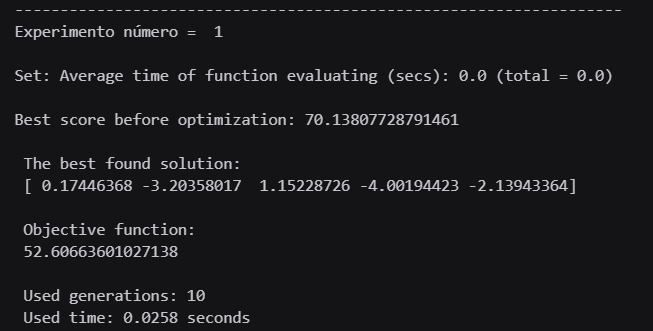
\includegraphics[scale = 0.75]{images/elitratio08_exp1.png}
                \caption{elit\_ratio = 0.8 - Experimento 1 }
            \end{figure}

            \begin{figure}[H]
                \centering
                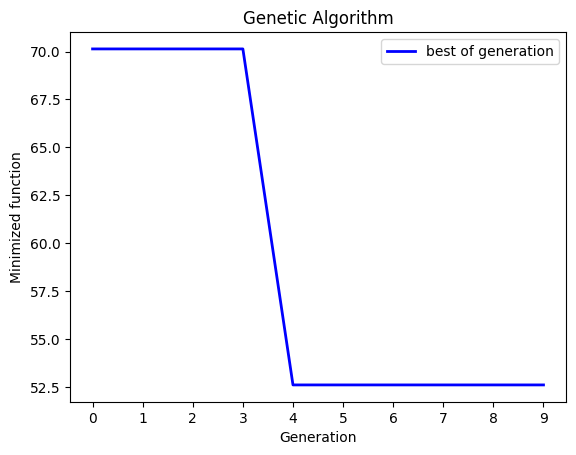
\includegraphics[scale = 0.75]{images/elitratio08_exp1_graphGA.png}
                \caption{Gráfico GA (elit\_ratio = 0.8 - Experimento 1) }
            \end{figure}

            \begin{figure}[H]
                \centering
                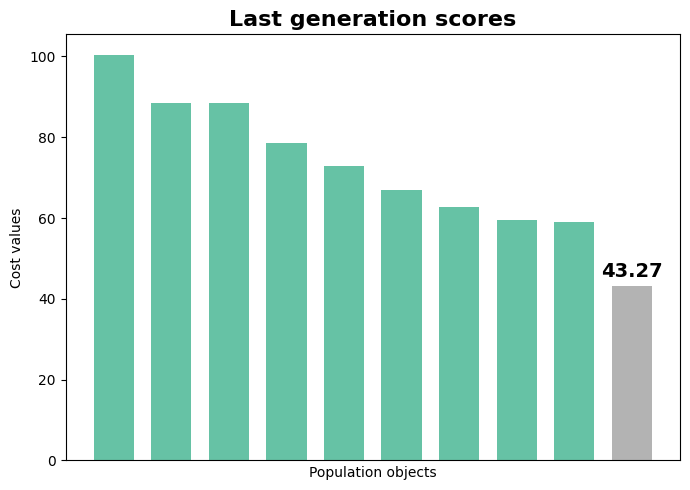
\includegraphics[scale = 0.75]{images/elitratio08_exp1_graphScore.png}
                \caption{Last Generation Scores (elit\_ratio = 0.8 - Experimento 1) }
            \end{figure}

            \textbf{Melhores indivíduos por geração}:\\
            
            [70.13807728791461,\\ 70.13807728791461,\\ 70.13807728791461,\\ 70.13807728791461,\\ 52.60663601027138,\\ 52.60663601027138,\\ 52.60663601027138,\\ 52.60663601027138,\\ 52.60663601027138,\\ 52.60663601027138]

        \newpage
        \item Experimento 2:
            \begin{figure}[H]
                \centering
                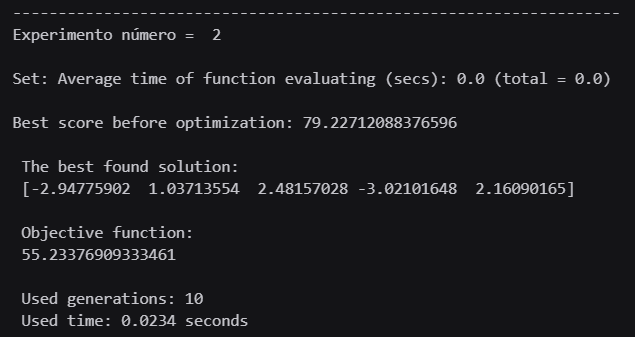
\includegraphics[scale = 0.75]{images/elitratio08_exp2.png}
                \caption{elit\_ratio = 0.8 - Experimento 2 }
            \end{figure}

            \begin{figure}[H]
                \centering
                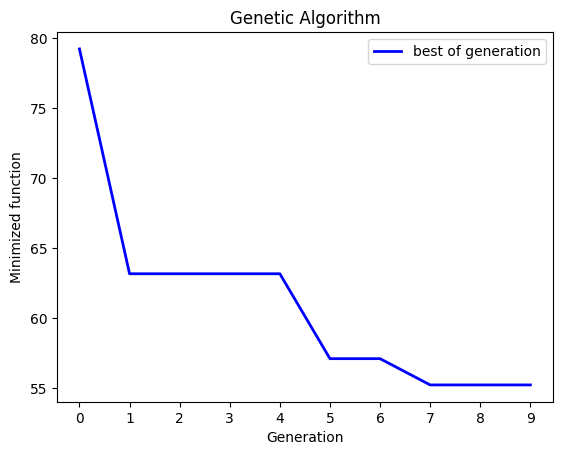
\includegraphics[scale = 0.75]{images/elitratio08_exp2_graphGA.png}
                \caption{Gráfico GA (elit\_ratio = 0.8 - Experimento 2) }
            \end{figure}

            \begin{figure}[H]
                \centering
                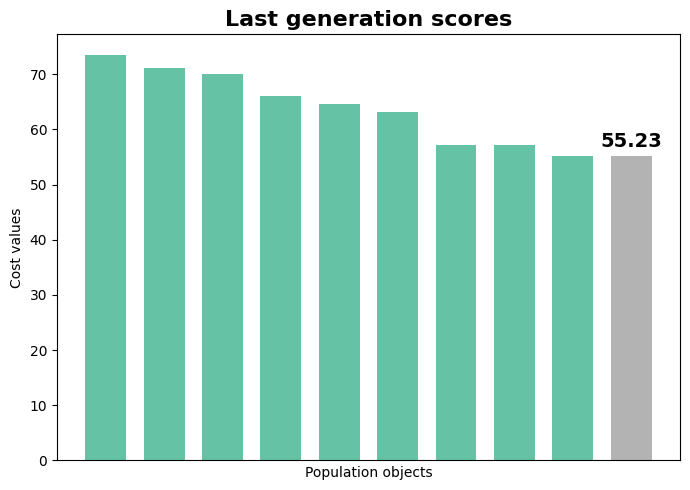
\includegraphics[scale = 0.75]{images/elitratio08_exp2_graphScore.png}
                \caption{Last Generation Scores (elit\_ratio = 0.8 - Experimento 2) }
            \end{figure}

            \textbf{Melhores indivíduos por geração}:\\
            
            [79.22712088376596,\\ 63.172243785468424,\\ 63.172243785468424,\\ 63.172243785468424,\\ 63.172243785468424,\\ 57.10829835768811,\\ 57.10829835768811,\\ 55.23376909333461,\\ 55.23376909333461,\\ 55.23376909333461] \\

            \textbf{elit\_ratio}: 0.8,\\
            
            \textbf{Média dos Melhores por Geração}:\\
            
            [74.68259908584028,\\ 66.65516053669151,\\ 66.65516053669151,\\ 66.65516053669151,\\ 57.889439897869906,\\ 54.85746718397975,\\ 54.85746718397975,\\ 53.920202551802994,\\ 53.920202551802994,\\ 53.920202551802994]
    \end{itemize}
\end{itemize}



\textbf{Interpretação dos Resultados}:\\

\begin{figure}[H]
    \centering
    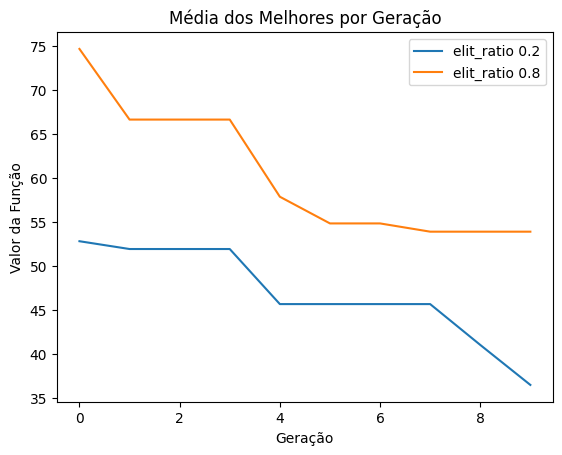
\includegraphics[scale = 0.75]{images/elitratio_graph_media.png}
    \caption{Gráfico comparativo - elit\_ratio }
\end{figure}

\begin{figure}[H]
    \centering
    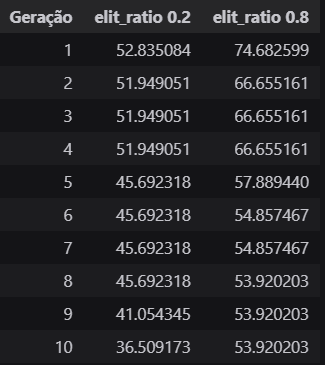
\includegraphics[scale = 0.90]{images/elitratio_tabela_comparativa.png}
    \caption{Tabela comparativa - elit\_ratio - média dos melhores }
\end{figure}


\begin{enumerate}
    \item \textbf{elit\_ratio= 0.2}:
    \begin{itemize}
        \item O gráfico representa uma menor proporção de elitismo (20\%). A função objetivo começa em torno de 52 e melhora lentamente ao longo das gerações, estabilizando em torno de 36 na 10ª geração.
        \item Permite maior diversidade genética, ajudando a explorar melhor o espaço de soluções e evitar a convergência prematura.
        \item Encontra soluções de melhor qualidade, com valores da função objetivo mais baixos.
        \item Tem uma convergência mais lenta, mas eventualmente encontra melhores soluções.
    \end{itemize}
    \item \textbf{elit\_ratio = 0.8}:
    \begin{itemize}
        \item  representa uma maior proporção de elitismo (80\%). A função objetivo começa mais alta, em torno de 74, mas também melhora rapidamente nas primeiras gerações.
        \item A convergência é mais rápida, mas os valores finais da função objetivo são mais altos em comparação com o elit\_ratio de 0.2.
        \item Resulta em menor diversidade genética, pois a maioria da população é preservada a cada geração, limitando a exploração.
        \item Permite maior diversidade genética, ajudando a explorar melhor o espaço de soluções e evitando a convergência prematura.
        \item Melhor para explorar o espaço de soluções de forma agressiva, encontrando soluções de alta qualidade.
    \end{itemize}
\end{enumerate}






\newpage
\subsubsection{Alternando a probabilidade de crossover (crossover\_probability)}


\begin{itemize}
    \item \textbf{crossover\_probability = 0.1}:
    \begin{itemize}
        \item Experimento 1:
            \begin{figure}[H]
                \centering
                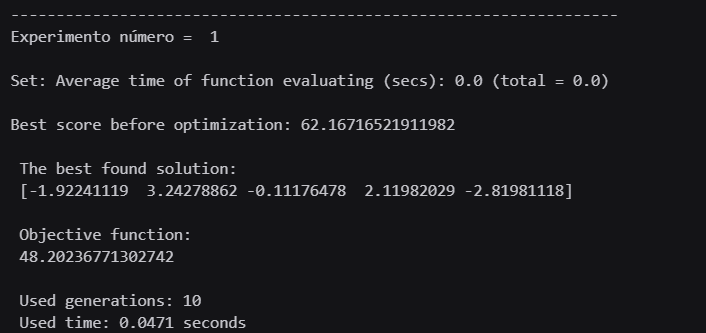
\includegraphics[scale = 0.75]{images/crosprob01_exp1.png}
                \caption{crossover\_probability = 0.1 - Experimento 1 }
            \end{figure}

            \begin{figure}[H]
                \centering
                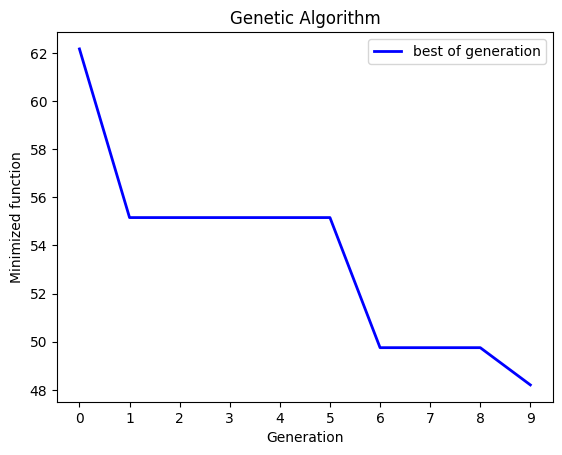
\includegraphics[scale = 0.75]{images/crosprob01_exp1_graphGA.png}
                \caption{Gráfico GA (crossover\_probability = 0.1 - Experimento 1) }
            \end{figure}

            \begin{figure}[H]
                \centering
                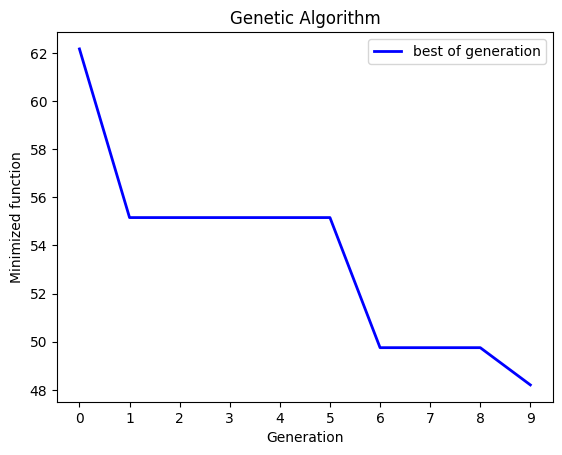
\includegraphics[scale = 0.75]{images/crosprob01_exp1_graphGA.png}
                \caption{Last Generation Scores (crossover\_probability = 0.1 - Experimento 1) }
            \end{figure}

            \textbf{Melhores indivíduos por geração}:\\
            
            [62.16716521911982,\\ 55.15750903723799,\\ 55.15750903723799,\\ 55.15750903723799,\\ 55.15750903723799,\\ 55.15750903723799,\\ 49.75071938833963,\\ 49.75071938833963,\\ 49.75071938833963,\\ 48.20236771302742]

        \newpage
        \item Experimento 2:
            \begin{figure}[H]
                \centering
                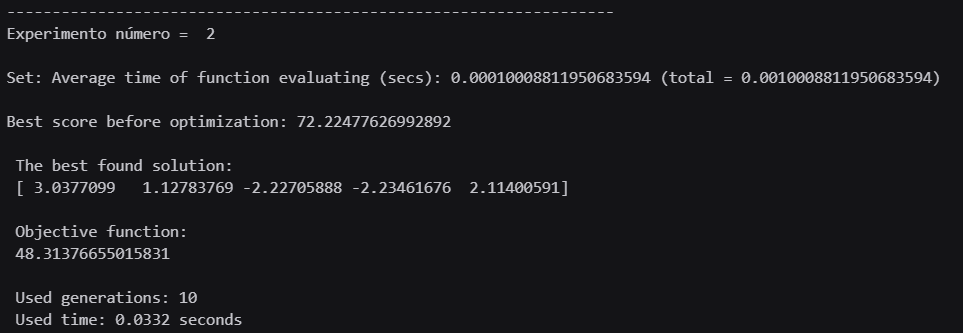
\includegraphics[scale = 0.75]{images/crosprob01_exp2.png}
                \caption{crossover\_probability = 0.1 - Experimento 2 }
            \end{figure}

            \begin{figure}[H]
                \centering
                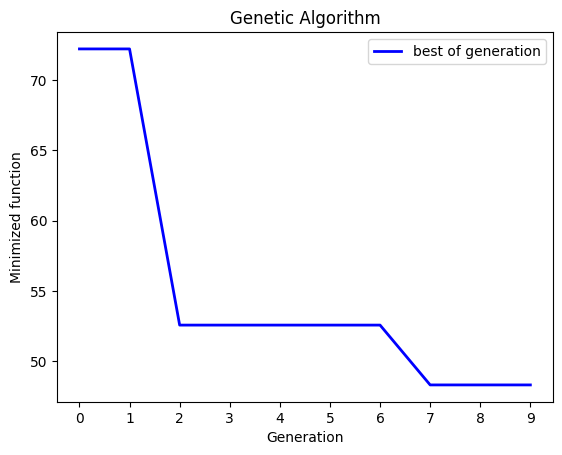
\includegraphics[scale = 0.75]{images/crosprob01_exp2_graphGA.png}
                \caption{Gráfico GA (crossover\_probability = 0.1 - Experimento 2) }
            \end{figure}

            \begin{figure}[H]
                \centering
                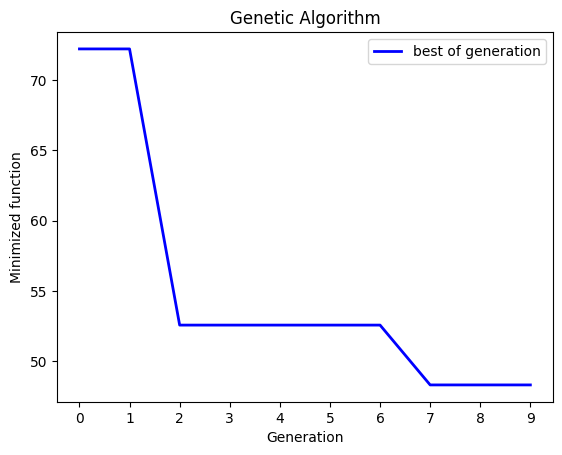
\includegraphics[scale = 0.75]{images/crosprob01_exp2_graphGA.png}
                \caption{Last Generation Scores (crossover\_probability = 0.1 - Experimento 2) }
            \end{figure}

            \textbf{Melhores indivíduos por geração}:\\
            
            [72.22477626992892,\\ 72.22477626992892,\\ 52.57129459511515,\\ 52.57129459511515,\\ 52.57129459511515,\\ 52.57129459511515,\\ 52.57129459511515,\\ 48.31376655015831, 48.31376655015831,\\ 48.31376655015831] \\

            \textbf{crossover\_probability}: 0.1,\\
            
            \textbf{Média dos Melhores por Geração}:\\
            
            [67.19597074452437,\\ 63.691142653583455,\\ 53.86440181617657,\\ 53.86440181617657,\\ 53.86440181617657,\\ 53.86440181617657,\\ 51.16100699172739,\\ 49.03224296924897,\\ 49.03224296924897,\\ 48.25806713159287]
    \end{itemize}
\end{itemize}



\begin{itemize}
    \item \textbf{crossover\_probability = 0.6}:
    \begin{itemize}
        \item Experimento 1:
            \begin{figure}[H]
                \centering
                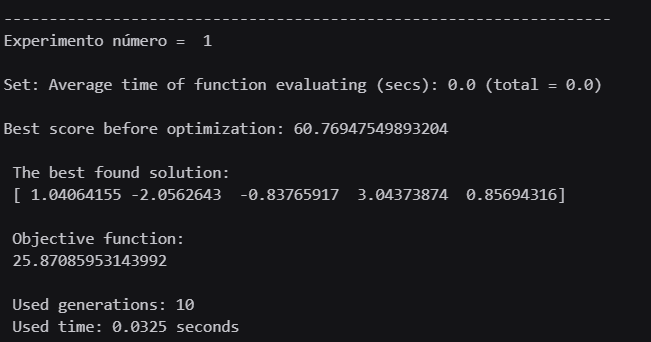
\includegraphics[scale = 0.75]{images/crosprob06_exp1.png}
                \caption{crossover\_probability = 0.6 - Experimento 1 }
            \end{figure}

            \begin{figure}[H]
                \centering
                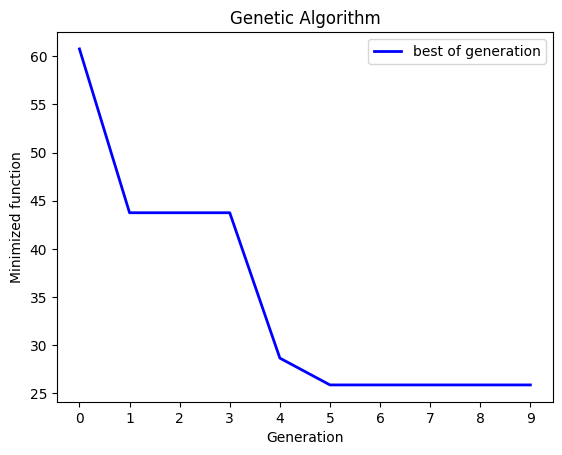
\includegraphics[scale = 0.75]{images/crosprob06_exp1_graphGA.png}
                \caption{Gráfico GA (crossover\_probability = 0.6 - Experimento 1) }
            \end{figure}

            \begin{figure}[H]
                \centering
                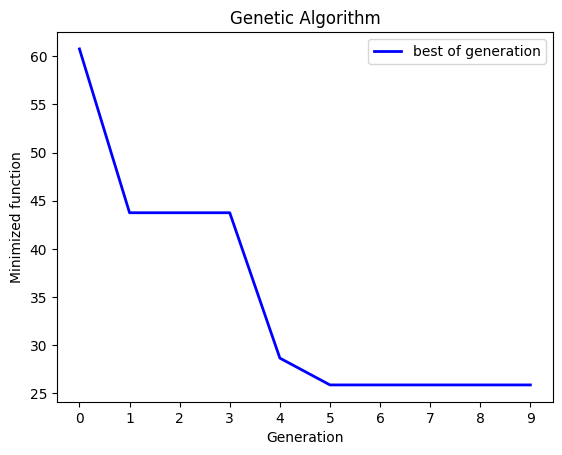
\includegraphics[scale = 0.75]{images/crosprob06_exp1_graphGA.png}
                \caption{Last Generation Scores (crossover\_probability = 0.6 - Experimento 1) }
            \end{figure}

            \textbf{Melhores indivíduos por geração}:\\
            
            [60.76947549893204,\\ 43.7548088772906,\\ 43.7548088772906,\\ 43.7548088772906,\\ 28.657239559994068,\\ 25.87085953143992,\\ 25.87085953143992,\\ 25.87085953143992,\\ 25.87085953143992,\\ 25.87085953143992]

        \newpage
        \item Experimento 2:
            \begin{figure}[H]
                \centering
                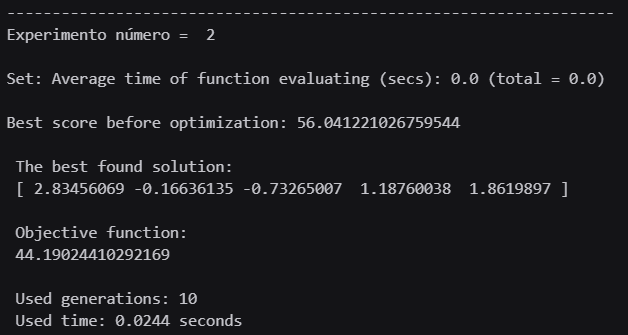
\includegraphics[scale = 0.75]{images/crosprob06_exp2.png}
                \caption{crossover\_probability = 0.6 - Experimento 2 }
            \end{figure}

            \begin{figure}[H]
                \centering
                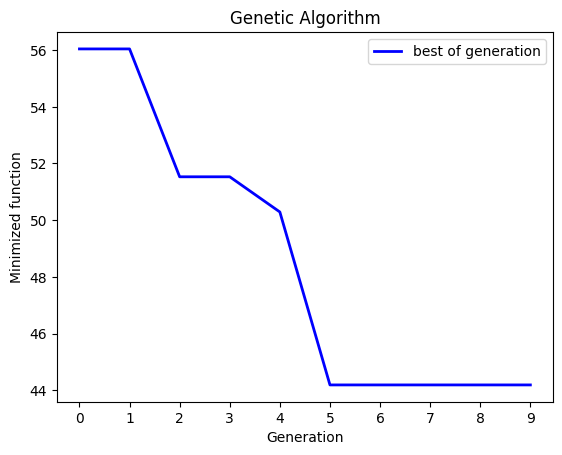
\includegraphics[scale = 0.75]{images/crosprob06_exp2_graphGA.png}
                \caption{Gráfico GA (crossover\_probability = 0.6 - Experimento 2) }
            \end{figure}

            \begin{figure}[H]
                \centering
                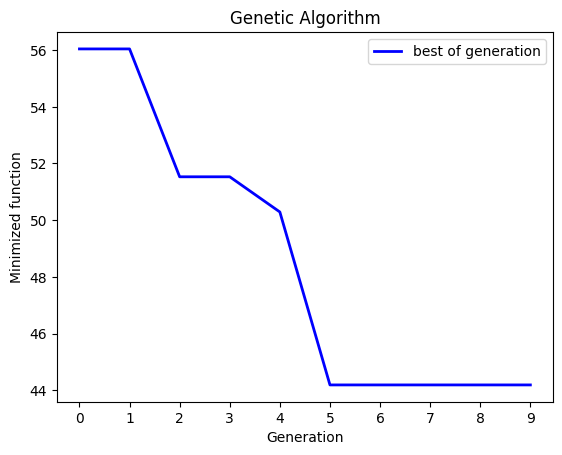
\includegraphics[scale = 0.75]{images/crosprob06_exp2_graphGA.png}
                \caption{Last Generation Scores (crossover\_probability = 0.6 - Experimento 2) }
            \end{figure}

            \textbf{Melhores indivíduos por geração}:\\
            
            [56.041221026759544,\\ 56.041221026759544,\\ 51.531115139022376,\\ 51.531115139022376,\\ 50.28972173562985,\\ 44.19024410292169,\\ 44.19024410292169,\\ 44.19024410292169,\\ 44.19024410292169,\\ 44.19024410292169] \\

            \textbf{crossover\_probability}: 0.6,\\
            
            \textbf{Média dos Melhores por Geração}:\\
            
            [58.40534826284579,\\ 49.89801495202507,\\ 47.64296200815649,\\ 47.64296200815649,\\ 39.473480647811954,\\ 35.03055181718081,\\ 35.03055181718081,\\ 35.03055181718081,\\ 35.03055181718081,\\ 35.03055181718081]
    \end{itemize}
\end{itemize}



\textbf{Interpretação dos Resultados}:\\

\begin{figure}[H]
    \centering
    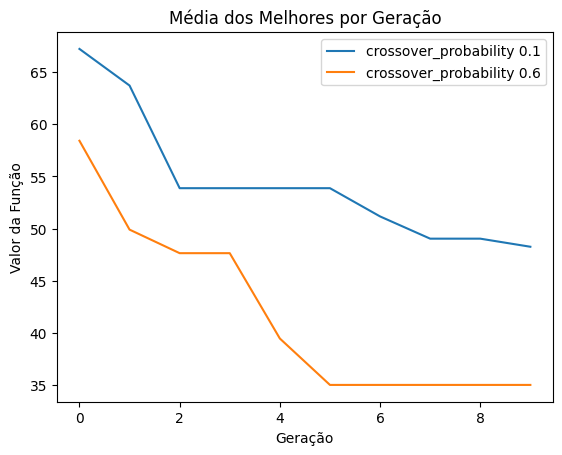
\includegraphics[scale = 0.75]{images/crosprob_graph_media.png}
    \caption{Gráfico comparativo - crossover\_probability }
\end{figure}

\begin{figure}[H]
    \centering
    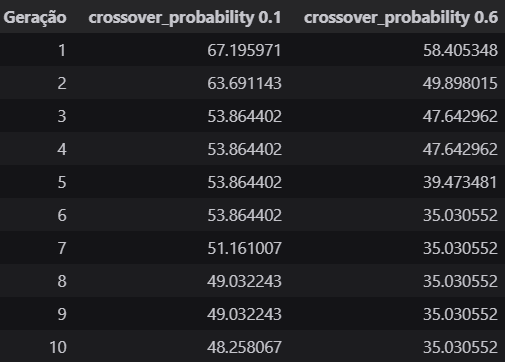
\includegraphics[scale = 0.90]{images/crosprob_tabela_comparativa.png}
    \caption{Tabela comparativa - crossover\_probability - média dos melhores }
\end{figure}


\begin{enumerate}
    \item \textbf{crossover\_probability = 0.1}:
    \begin{itemize}
        \item A função objetivo começa em torno de 67 e melhora ao longo das gerações. A convergência é mais lenta e a função objetivo estabiliza em torno de 48 na 10ª geração.
        \item Resulta em menor diversidade genética, limitando a exploração.
        \item Adequado para cenários onde a estabilidade e uma convergência mais controlada são preferidas.
        \item Convergência mais lenta e mas resultados finais menos ótimos.
    \end{itemize}
    \item \textbf{crossover\_probability = 0.6}:
    \begin{itemize}
        \item  A função objetivo começa em torno de 58 e melhora rapidamente nas primeiras gerações.
        \item A função objetivo melhora rapidamente nas primeiras gerações, indicando uma rápida convergência inicial.
        \item A convergência é mais rápida e a função objetivo estabiliza em torno de 35 na 6ª geração.
        \item a função objetivo estabiliza em um valor mais baixo, em torno de 35.
        \item Permite maior diversidade genética, ajudando a explorar melhor o espaço de soluções e evitando a convergência prematura.
        \item Melhor para explorar o espaço de soluções de forma mais agressiva, encontrando soluções de alta qualidade rapidamente.
        \item Resultados finais melhores.
        
    \end{itemize}
\end{enumerate}






\newpage
\subsubsection{Alternando a proporção de pais (parents\_portion)}


\begin{itemize}
    \item \textbf{parents\_portion = 0.2}:
    \begin{itemize}
        \item Experimento 1:
            \begin{figure}[H]
                \centering
                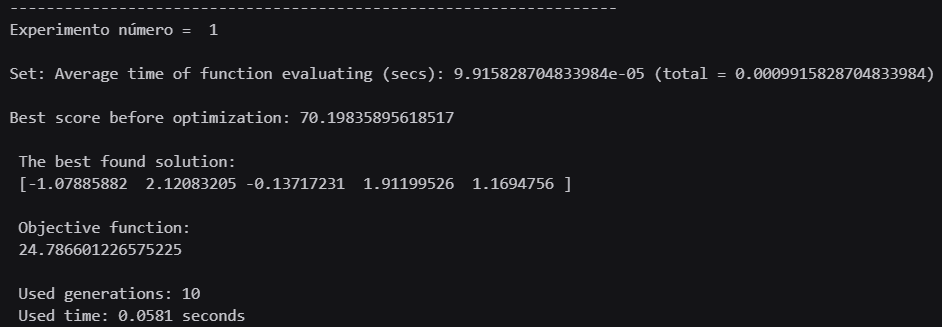
\includegraphics[scale = 0.75]{images/parents02_exp1.png}
                \caption{parents\_portion = 0.2 - Experimento 1 }
            \end{figure}

            \begin{figure}[H]
                \centering
                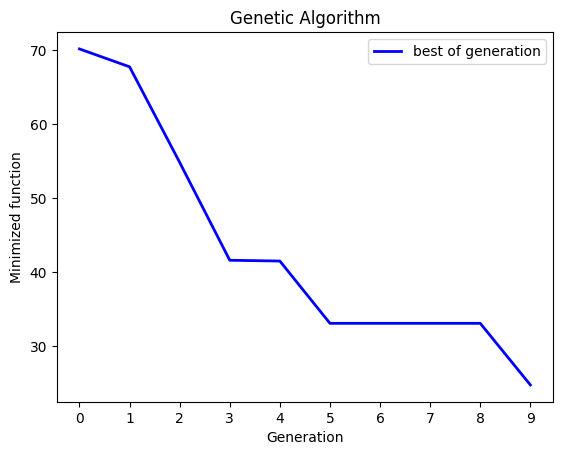
\includegraphics[scale = 0.75]{images/parents02_exp1_graphGA.png}
                \caption{Gráfico GA (parents\_portion = 0.2 - Experimento 1) }
            \end{figure}

            \begin{figure}[H]
                \centering
                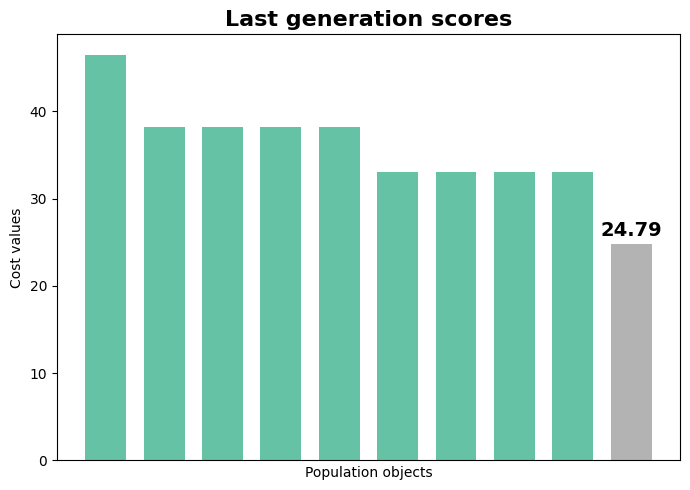
\includegraphics[scale = 0.75]{images/parents02_exp1_graphScore.png}
                \caption{Last Generation Scores (parents\_portion = 0.2 - Experimento 1) }
            \end{figure}

            \textbf{Melhores indivíduos por geração}:\\
            
            [70.19835895618517,\\ 67.78067489608723,\\ 54.86785332642501,\\ 41.63584814757107,\\ 41.529975720016964,\\ 33.1127470568957,\\ 33.1127470568957,\\ 33.1127470568957,\\ 33.1127470568957,\\ 24.786601226575225]

        \newpage
        \item Experimento 2:
            \begin{figure}[H]
                \centering
                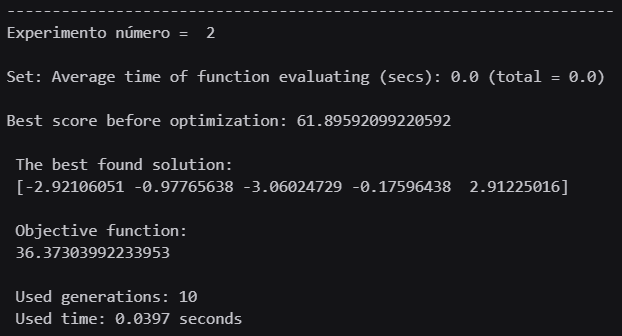
\includegraphics[scale = 0.75]{images/parents02_exp2.png}
                \caption{parents\_portion = 0.2 - Experimento 2 }
            \end{figure}

            \begin{figure}[H]
                \centering
                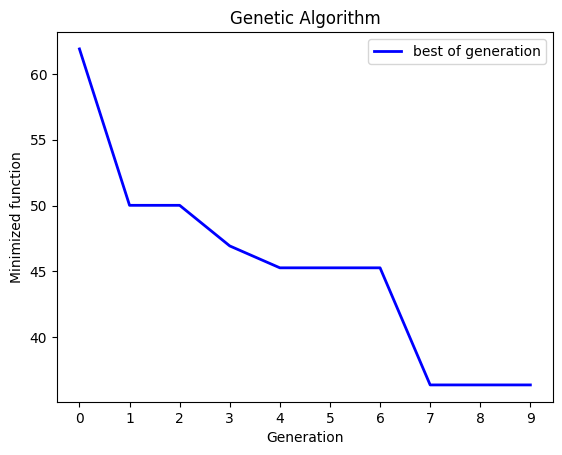
\includegraphics[scale = 0.75]{images/parents02_exp2_graphGA.png}
                \caption{Gráfico GA (parents\_portion = 0.2 - Experimento 2) }
            \end{figure}

            \begin{figure}[H]
                \centering
                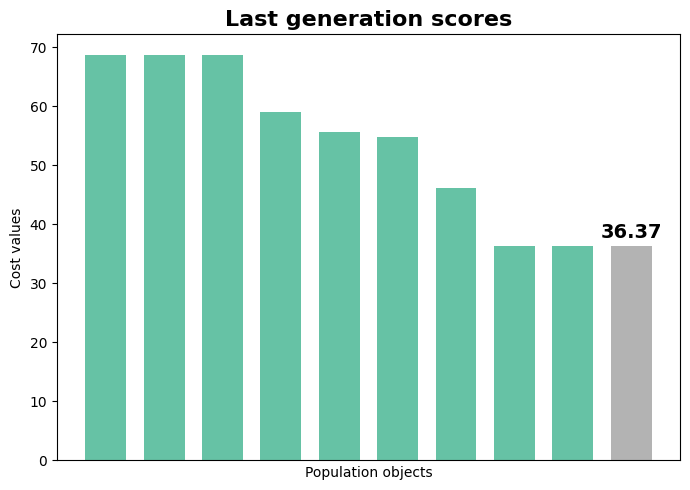
\includegraphics[scale = 0.75]{images/parents02_exp2_graphScore.png}
                \caption{Last Generation Scores (parents\_portion = 0.2 - Experimento 2) }
            \end{figure}

            \textbf{Melhores indivíduos por geração}:\\
            
            [61.89592099220592,\\ 50.015742608698304,\\ 50.015742608698304,\\ 46.93070793395578,\\ 45.268070103496264,\\ 45.268070103496264,\\ 45.268070103496264,\\ 36.37303992233953,\\ 36.37303992233953,\\ 36.37303992233953] \\

            \textbf{parents\_portion}: 0.2,\\
            
            \textbf{Média dos Melhores por Geração}:\\
            
            [66.04713997419555,\\ 58.89820875239277,\\ 52.441797967561655,\\ 44.28327804076342,\\ 43.39902291175662,\\ 39.19040858019598,\\ 39.19040858019598,\\ 34.742893489617614,\\ 34.742893489617614,\\ 30.57982057445738]
    \end{itemize}
\end{itemize}

\newpage
\begin{itemize}
    \item \textbf{parents\_portion = 0.8}:
    \begin{itemize}
        \item Experimento 1:
            \begin{figure}[H]
                \centering
                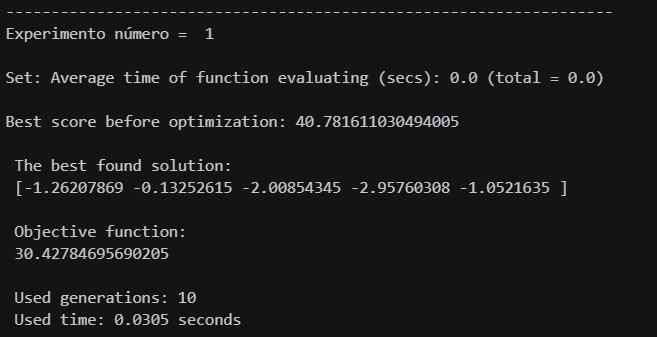
\includegraphics[scale = 0.75]{images/parents08_exp1.png}
                \caption{parents\_portion = 0.8 - Experimento 1 }
            \end{figure}

            \begin{figure}[H]
                \centering
                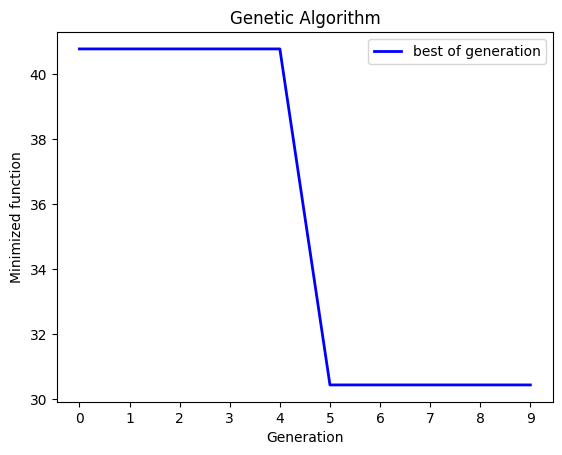
\includegraphics[scale = 0.75]{images/parents08_exp1_graphGA.png}
                \caption{Gráfico GA (parents\_portion = 0.8 - Experimento 1) }
            \end{figure}

            \begin{figure}[H]
                \centering
                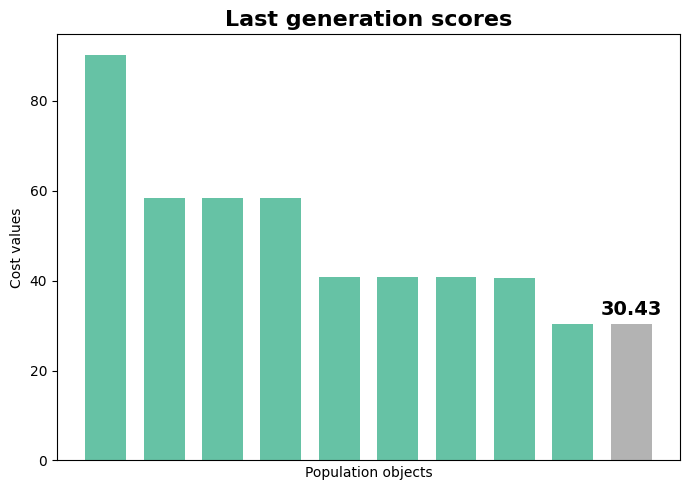
\includegraphics[scale = 0.75]{images/parents08_exp1_graphScore.png}
                \caption{Last Generation Scores (parents\_portion = 0.8 - Experimento 1) }
            \end{figure}

            \textbf{Melhores indivíduos por geração}:\\
            
            [40.781611030494005,\\ 40.781611030494005,\\ 40.781611030494005,\\ 40.781611030494005,\\ 40.781611030494005,\\ 30.42784695690205,\\ 30.42784695690205,\\ 30.42784695690205,\\ 30.42784695690205,\\ 30.42784695690205]

        \newpage
        \item Experimento 2:
            \begin{figure}[H]
                \centering
                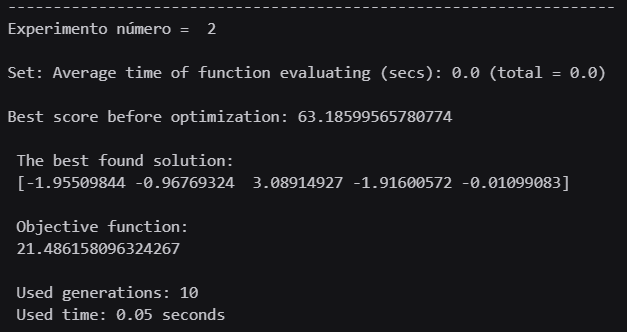
\includegraphics[scale = 0.75]{images/parents08_exp2.png}
                \caption{parents\_portion = 0.8 - Experimento 2 }
            \end{figure}

            \begin{figure}[H]
                \centering
                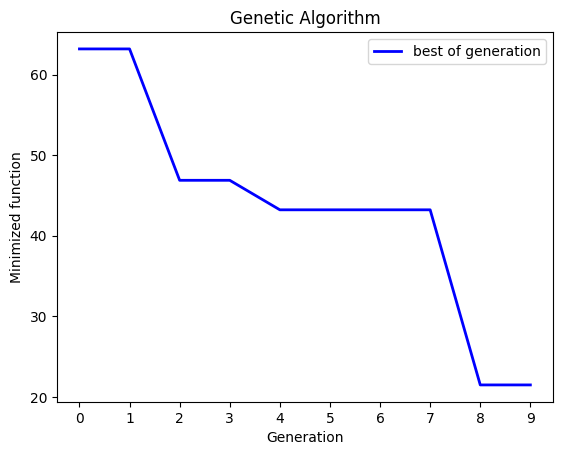
\includegraphics[scale = 0.75]{images/parents08_exp2_graphGA.png}
                \caption{Gráfico GA (parents\_portion = 0.8 - Experimento 2) }
            \end{figure}

            \begin{figure}[H]
                \centering
                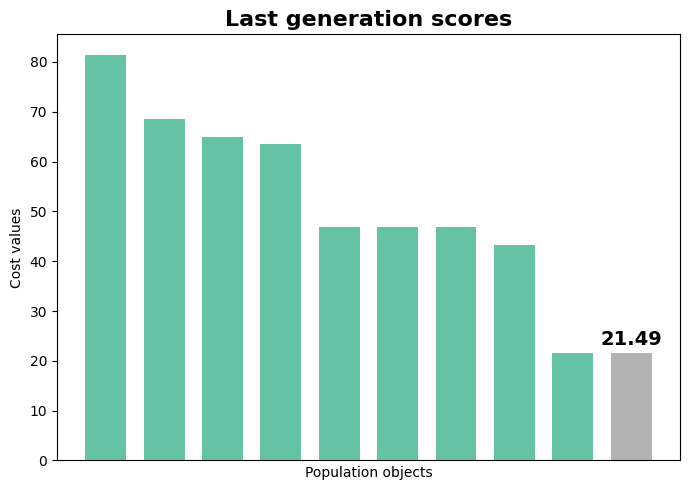
\includegraphics[scale = 0.75]{images/parents08_exp2_graphScore.png}
                \caption{Last Generation Scores (parents\_portion = 0.8 - Experimento 2) }
            \end{figure}

            \textbf{Melhores indivíduos por geração}:\\
            
            [63.18599565780774,\\ 63.18599565780774,\\ 46.88054840078859,\\ 46.88054840078859,\\ 43.21834137070964,\\ 43.21834137070964,\\ 43.21834137070964,\\ 43.21834137070964,\\ 21.486158096324267,\\ 21.486158096324267] \\

            \textbf{parents\_portion}: 0.8,\\
            
            \textbf{Média dos Melhores por Geração}:\\
            
            [51.98380334415087,\\ 51.98380334415087,\\ 43.831079715641295,\\ 43.831079715641295,\\ 41.99997620060182,\\ 36.82309416380585,\\ 36.82309416380585,\\ 36.82309416380585,\\ 25.95700252661316,\\ 25.95700252661316]
    \end{itemize}
\end{itemize}



\textbf{Interpretação dos Resultados}:\\

\begin{figure}[H]
    \centering
    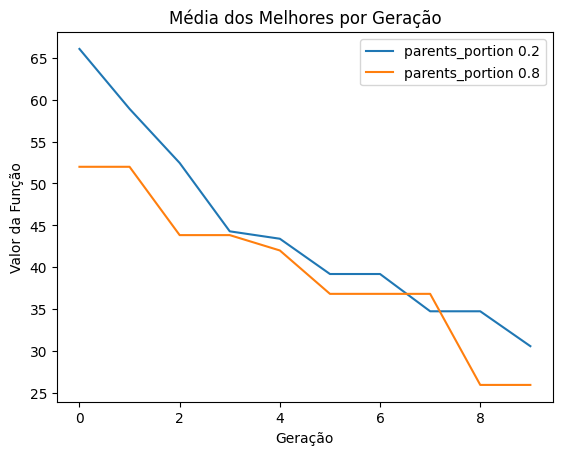
\includegraphics[scale = 0.75]{images/parents_graph_media.png}
    \caption{Gráfico comparativo - parents\_portion }
\end{figure}

\begin{figure}[H]
    \centering
    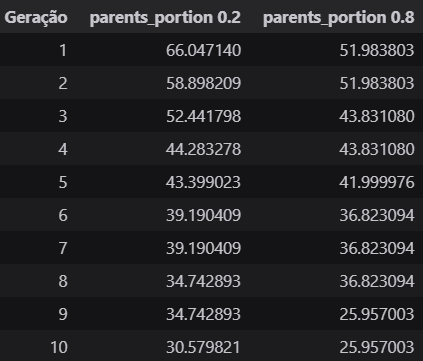
\includegraphics[scale = 0.90]{images/parents_tabela_comparativa.png}
    \caption{Tabela comparativa - parents\_portion - média dos melhores }
\end{figure}


\begin{enumerate}
    \item \textbf{parents\_portion = 0.2}:
    \begin{itemize}
        \item A função objetivo melhora de forma mais gradual. Continua a melhorar ao longo das gerações, chegando a um valor final de aproximadamente 30.
        \item Permite maior diversidade genética, ajudando a explorar melhor o espaço de soluções e evitando a convergência prematura.
        \item Adequado para cenários onde a exploração do espaço de soluções é crucial e as melhores soluções são desejadas.
    \end{itemize}
    \item \textbf{parents\_portion = 0.8}:
    \begin{itemize}
        \item  A função objetivo começa em torno de 52 e melhora rapidamente nas primeiras gerações.
        \item A convergência é mais rápida e a função objetivo estabiliza em torno de 26 na 9ª geração.
        \item Resulta em menor diversidade genética, pois uma maior parte da população é composta por pais, limitando a exploração.
        \item Melhor para cenários onde a estabilidade e uma rápida convergência inicial são preferidas. 
        \item Convergência rápida, com resultados finais bons, mas com potencial de melhoria limitado a longo prazo.
        
    \end{itemize}
\end{enumerate}








\newpage
\subsubsection{Alternando o tipo de crossover (crossover\_type)}

\begin{itemize}
    \item \textbf{Crossover de 1 ponto}:
    \begin{itemize}
        \item Experimento 1:
            \begin{figure}[H]
                \centering
                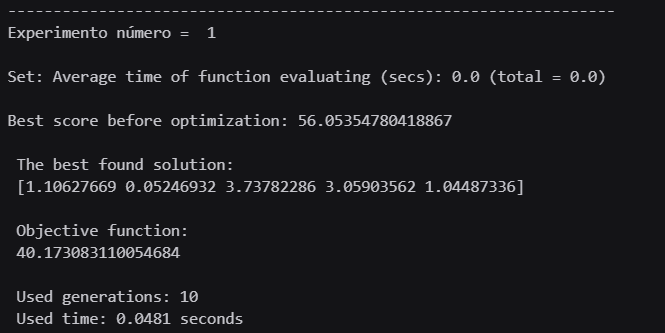
\includegraphics[scale = 0.75]{images/crostype1p_exp1.png}
                \caption{Crossover de 1 ponto - Experimento 1 }
            \end{figure}

            \begin{figure}[H]
                \centering
                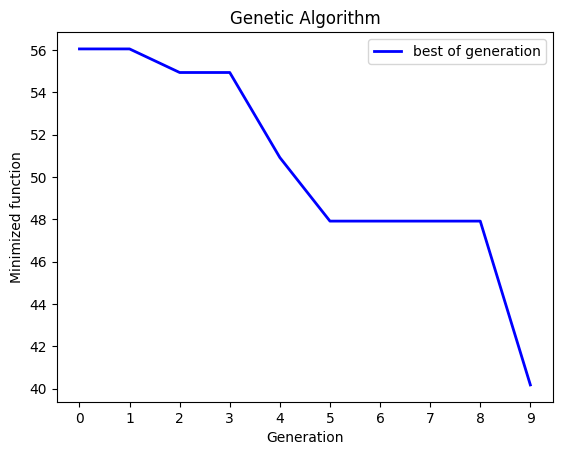
\includegraphics[scale = 0.75]{images/crostype1p_exp1_graphGA.png}
                \caption{Gráfico GA (Crossover de 1 ponto - Experimento 1) }
            \end{figure}

            \begin{figure}[H]
                \centering
                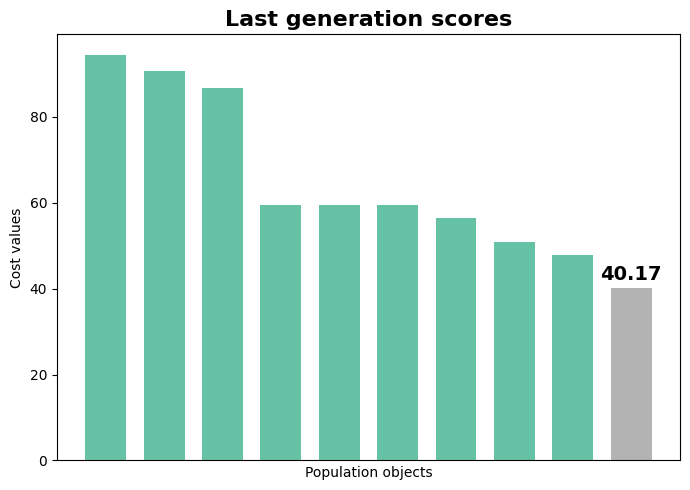
\includegraphics[scale = 0.75]{images/crostype1p_exp1_graphScore.png}
                \caption{Last Generation Scores (Crossover de 1 ponto - Experimento 1) }
            \end{figure}

            \textbf{Melhores indivíduos por geração}:\\
            
            [56.05354780418867,\\ 56.05354780418867,\\ 54.93904526092261,\\ 54.93904526092261,\\ 50.92014971118591,\\ 47.91542982778648,\\ 47.91542982778648,\\ 47.91542982778648,\\ 47.91542982778648,\\ 40.173083110054684]

        \newpage
        \item Experimento 2:
            \begin{figure}[H]
                \centering
                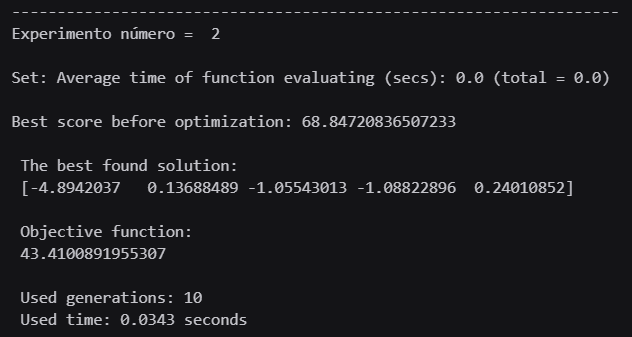
\includegraphics[scale = 0.75]{images/crostype1p_exp2.png}
                \caption{Crossover de 1 ponto - Experimento 2 }
            \end{figure}

            \begin{figure}[H]
                \centering
                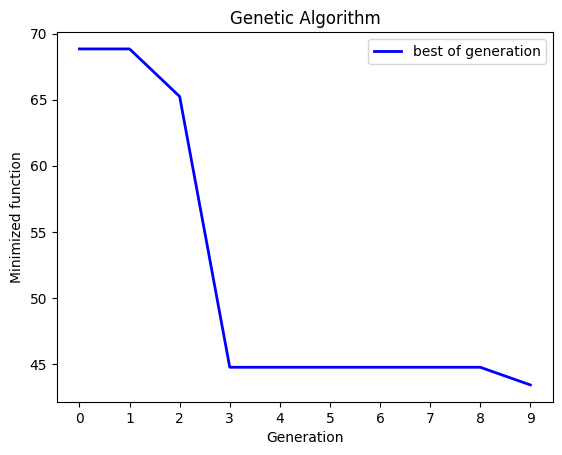
\includegraphics[scale = 0.75]{images/crostype1p_exp2_graphGA.png}
                \caption{Gráfico GA (Crossover de 1 ponto - Experimento 2) }
            \end{figure}

            \begin{figure}[H]
                \centering
                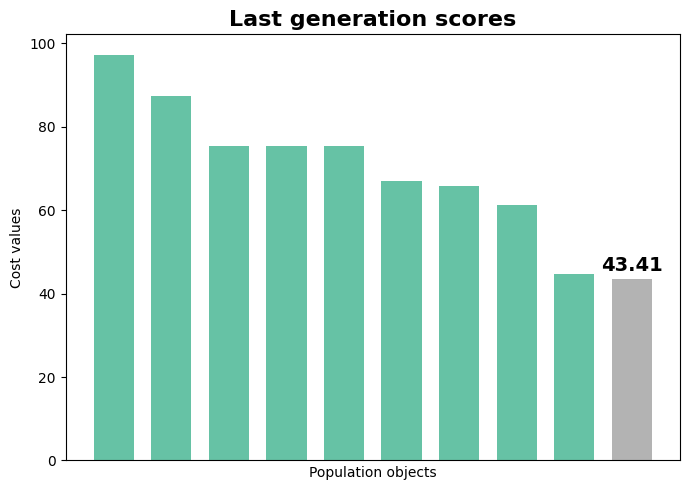
\includegraphics[scale = 0.75]{images/crostype1p_exp2_graphScore.png}
                \caption{Last Generation Scores (Crossover de 1 ponto - Experimento 2) }
            \end{figure}

            \textbf{Melhores indivíduos por geração}:\\
            
            [68.84720836507233,\\ 68.84720836507233,\\ 65.24566085330335,\\ 44.747187748518726,\\ 44.747187748518726,\\ 44.747187748518726,\\ 44.747187748518726,\\ 44.747187748518726,\\ 44.747187748518726,\\ 43.4100891955307] \\

            \textbf{Tipo de Crossover}: 1 ponto,\\
            
            \textbf{Média dos Melhores por Geração}:\\
            
            [62.4503780846305,\\ 62.4503780846305,\\ 60.09235305711298,\\ 49.84311650472067,\\ 47.83366872985232,\\ 46.331308788152604,\\ 46.331308788152604,\\ 46.331308788152604,\\ 46.331308788152604,\\ 41.79158615279269]
    \end{itemize}
\end{itemize}


\begin{itemize}
    \item \textbf{Crossover de 2 pontos}:
    \begin{itemize}
        \item Experimento 1:
            \begin{figure}[H]
                \centering
                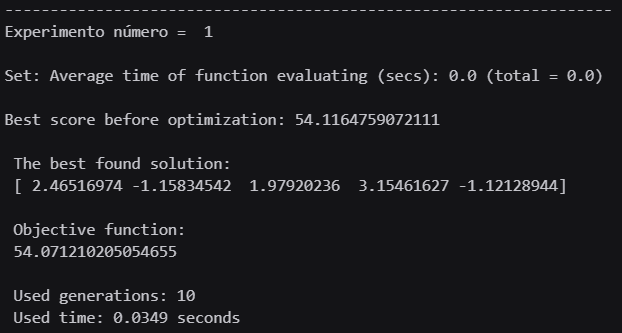
\includegraphics[scale = 0.75]{images/crostype2p_exp1.png}
                \caption{Crossover de 2 pontos - Experimento 1 }
            \end{figure}

            \begin{figure}[H]
                \centering
                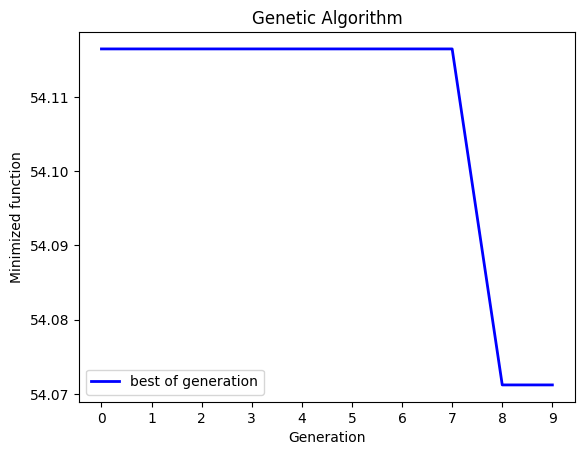
\includegraphics[scale = 0.75]{images/crostype2p_exp1_graphGA.png}
                \caption{Gráfico GA (Crossover de 2 pontos - Experimento 1) }
            \end{figure}

            \begin{figure}[H]
                \centering
                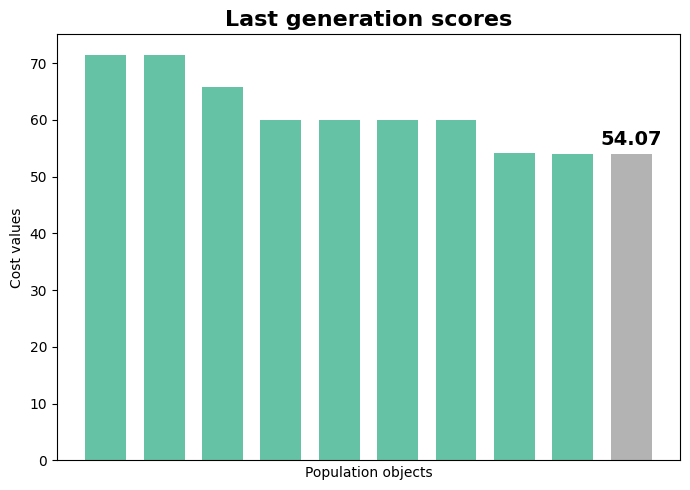
\includegraphics[scale = 0.75]{images/crostype2p_exp1_graphScore.png}
                \caption{Last Generation Scores (Crossover de 2 pontos - Experimento 1) }
            \end{figure}

            \textbf{Melhores indivíduos por geração}:\\
            
            [54.1164759072111,\\ 54.1164759072111,\\ 54.1164759072111,\\ 54.1164759072111,\\ 54.1164759072111,\\ 54.1164759072111,\\ 54.1164759072111,\\ 54.1164759072111,\\ 54.071210205054655,\\ 54.071210205054655]

        \newpage
        \item Experimento 2:
            \begin{figure}[H]
                \centering
                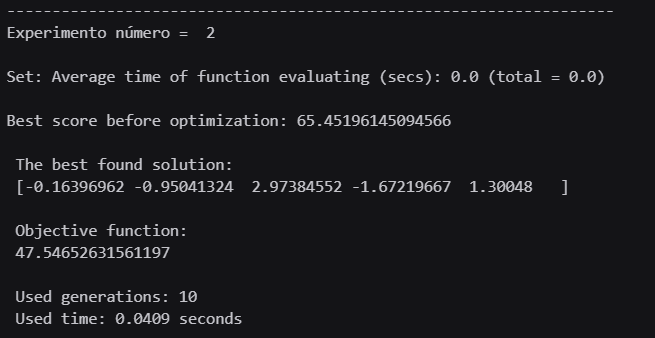
\includegraphics[scale = 0.75]{images/crostype2p_exp2.png}
                \caption{Crossover de 2 pontos - Experimento 2 }
            \end{figure}

            \begin{figure}[H]
                \centering
                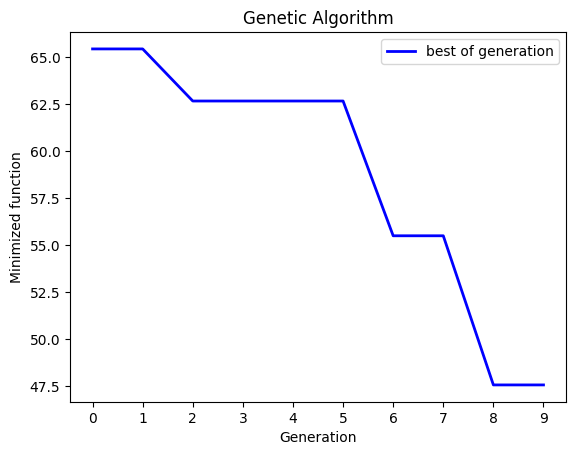
\includegraphics[scale = 0.75]{images/crostype2p_exp2_graphGA.png}
                \caption{Gráfico GA (Crossover de 2 pontos - Experimento 2) }
            \end{figure}

            \begin{figure}[H]
                \centering
                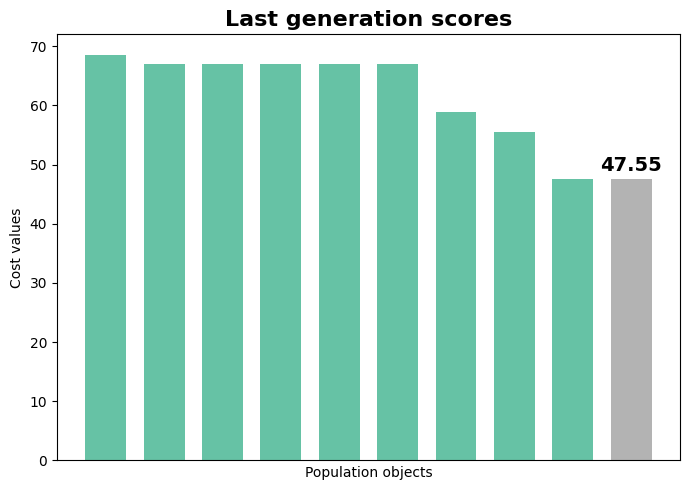
\includegraphics[scale = 0.75]{images/crostype2p_exp2_graphScore.png}
                \caption{Last Generation Scores (Crossover de 2 pontos - Experimento 2) }
            \end{figure}

            \textbf{Melhores indivíduos por geração}:\\
            
            [65.45196145094566,\\ 65.45196145094566,\\ 62.67604410342457,\\ 62.67604410342457,\\ 62.67604410342457,\\ 62.67604410342457,\\ 55.49427496508655,\\ 55.49427496508655,\\ 47.54652631561197,\\ 47.54652631561197] \\

            \textbf{Tipo de Crossover}: 2 pontos,\\
            
            \textbf{Média dos Melhores por Geração}:\\
            
            [59.78421867907838,\\ 59.78421867907838,\\ 58.396260005317835,\\ 58.396260005317835,\\ 58.396260005317835,\\ 58.396260005317835,\\ 54.80537543614882,\\ 54.80537543614882,\\ 50.80886826033331,\\ 50.80886826033331]
    \end{itemize}
\end{itemize}


\begin{itemize}
    \item \textbf{Crossover Uniforme}:
    \begin{itemize}
        \item Experimento 1:
            \begin{figure}[H]
                \centering
                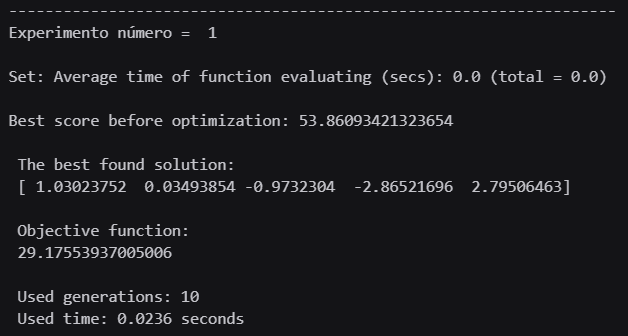
\includegraphics[scale = 0.75]{images/crostypeUni_exp1.png}
                \caption{Crossover Uniforme - Experimento 1 }
            \end{figure}

            \begin{figure}[H]
                \centering
                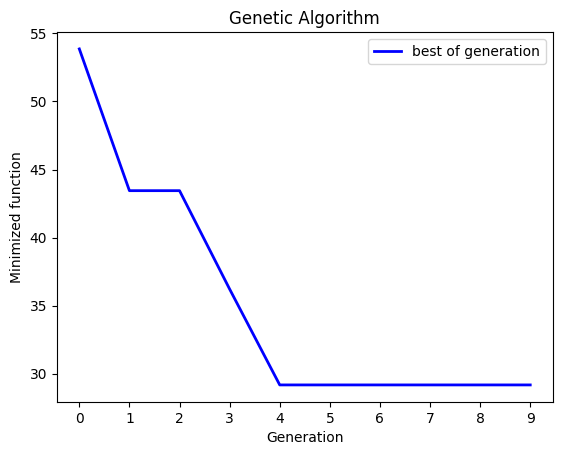
\includegraphics[scale = 0.75]{images/crostypeUni_exp1_graphGA.png}
                \caption{Gráfico GA (Crossover Uniforme - Experimento 1) }
            \end{figure}

            \begin{figure}[H]
                \centering
                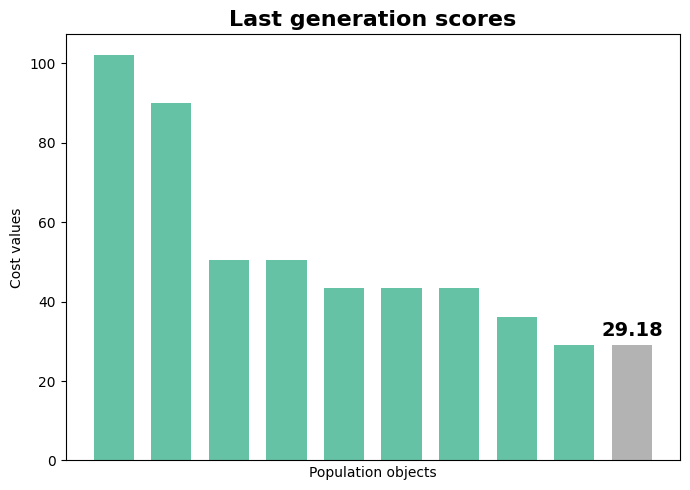
\includegraphics[scale = 0.75]{images/crostypeUni_exp1_graphScore.png}
                \caption{Last Generation Scores (Crossover Uniforme - Experimento 1) }
            \end{figure}

            \textbf{Melhores indivíduos por geração}:\\
            
            [53.86093421323654,\\ 43.447282490013606,\\ 43.447282490013606,\\ 36.215656480120614,\\ 29.17553937005006,\\ 29.17553937005006,\\ 29.17553937005006,\\ 29.17553937005006,\\ 29.17553937005006,\\ 29.17553937005006]

        \newpage
        \item Experimento 2:
            \begin{figure}[H]
                \centering
                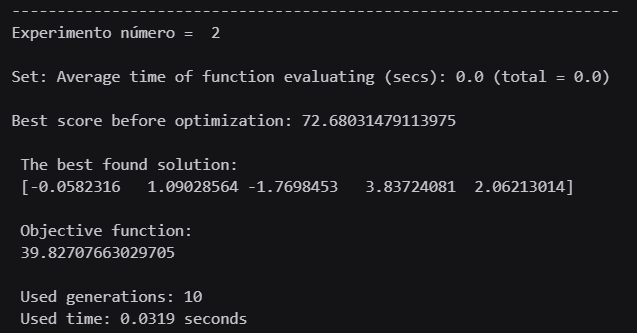
\includegraphics[scale = 0.75]{images/crostypeUni_exp2.png}
                \caption{Crossover Uniforme - Experimento 2 }
            \end{figure}

            \begin{figure}[H]
                \centering
                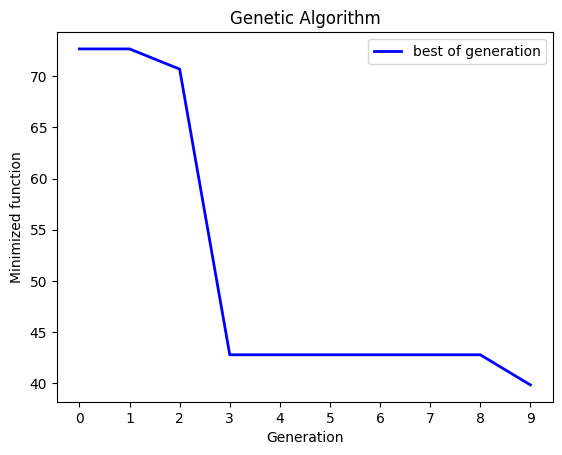
\includegraphics[scale = 0.75]{images/crostypeUni_exp2_graphGA.png}
                \caption{Gráfico GA (Crossover Uniforme - Experimento 2) }
            \end{figure}

            \begin{figure}[H]
                \centering
                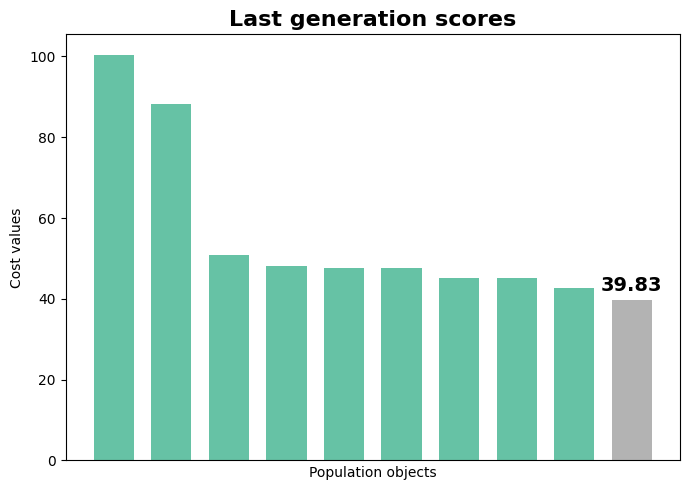
\includegraphics[scale = 0.75]{images/crostypeUni_exp2_graphScore.png}
                \caption{Last Generation Scores (Crossover Uniforme - Experimento 2) }
            \end{figure}

            \textbf{Melhores indivíduos por geração}:\\
            
            [72.68031479113975,\\ 72.68031479113975,\\ 70.70471755647274,\\ 42.77549122129812,\\ 42.77549122129812,\\ 42.77549122129812,\\ 42.77549122129812,\\ 42.77549122129812,\\ 42.77549122129812,\\ 39.82707663029705] \\

            \textbf{Tipo de Crossover}: uniforme,\\
            
            \textbf{Média dos Melhores por Geração}:\\
            
            [63.27062450218814,\\ 58.06379864057668,\\ 57.076000023243175,\\ 39.49557385070936,\\ 35.975515295674086,\\ 35.975515295674086,\\ 35.975515295674086,\\ 35.975515295674086,\\ 35.975515295674086,\\ 34.50130800017355]
    \end{itemize}
\end{itemize}



\textbf{Interpretação dos Resultados}:\\

\begin{figure}[H]
    \centering
    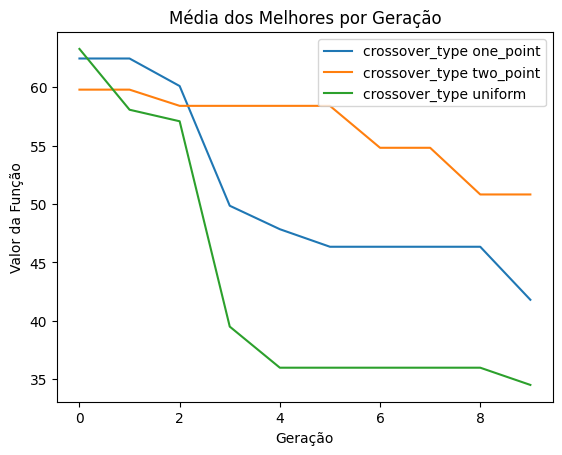
\includegraphics[scale = 0.75]{images/crostype_graph_media.png}
    \caption{Gráfico comparativo - Tipo de Crossover }
\end{figure}

\begin{figure}[H]
    \centering
    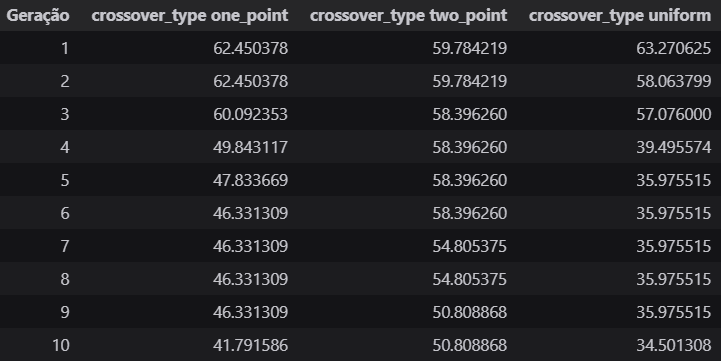
\includegraphics[scale = 0.90]{images/crostype_tabela_comparativa.png}
    \caption{Tabela comparativa - Tipo de Crossover - média dos melhores }
\end{figure}

\begin{enumerate}
    \item \textbf{Crossover de 1 ponto}:
    \begin{itemize}
        \item A convergência é mais lenta, mas os valores da função objetivo continuam a melhorar até a 10ª geração, chegando a um valor de aproximadamente 41.

        \item Adequado para cenários onde a estabilidade e uma convergência mais controlada são preferidas.
        \item Convergência mais lenta, mas permite encontrar soluções melhores ao longo do tempo.
    \end{itemize}
    \item \textbf{Crossover de dois pontos}:
    \begin{itemize}
        \item A convergência é mais rápida comparado ao crossover de 1 ponto, mas os valores da função objetivo estabilizam em torno de 50. A função objetivo melhora rapidamente, mas estabiliza em um valor intermediário.
        \item Assim como o \textit{one point crossover}, resulta em menor diversidade genética, limitando a exploração.
        \item Adequado para cenários onde uma convergência intermediária é desejada. A Convergência é rápida, mas com potencial de melhoria limitado a longo prazo.
    \end{itemize}
    \item \textbf{Crossover Uniforme}
    \begin{itemize}
        \item A função objetivo começa em torno de 63 e melhora de forma significativa nas primeiras gerações. A convergência é mais rápida e os valores da função objetivo estabilizam em torno de 34.
        \item Permite maior diversidade genética, ajudando a explorar melhor o espaço de soluções e evitando a convergência prematura.
        \item Melhor para explorar o espaço de soluções de forma mais agressiva, encontrando soluções de alta qualidade rapidamente.
        \item Convergência rápida, com resultados finais melhores.
    \end{itemize}
        
    
\end{enumerate}





\newpage
\subsubsection{Alternando o tipo de mutação (mutation\_type)}


\begin{itemize}
    \item \textbf{Tipo de Mutação = uniform\_by\_center}:
    \begin{itemize}
        \item Experimento 1:
            \begin{figure}[H]
                \centering
                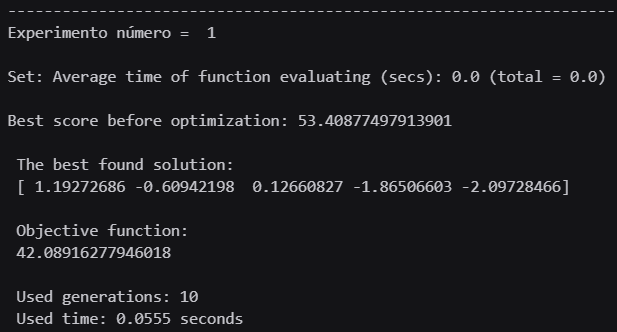
\includegraphics[scale = 0.75]{images/mutype_ubc_exp1.png}
                \caption{Tipo de Mutação = uniform\_by\_center - Experimento 1 }
            \end{figure}

            \begin{figure}[H]
                \centering
                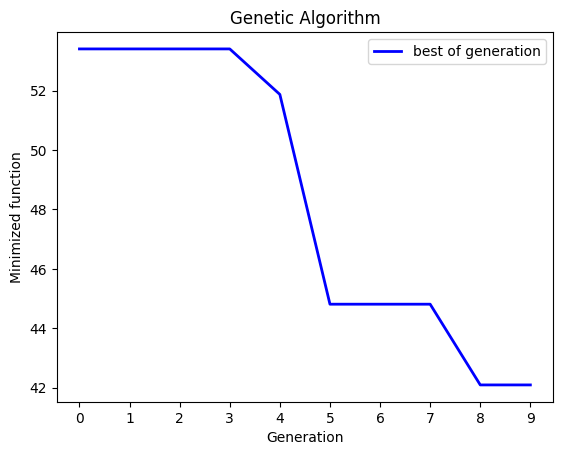
\includegraphics[scale = 0.75]{images/mutype_ubc_exp1_graphGA.png}
                \caption{Gráfico GA (CTipo de Mutação = uniform\_by\_center - Experimento 1) }
            \end{figure}

            \begin{figure}[H]
                \centering
                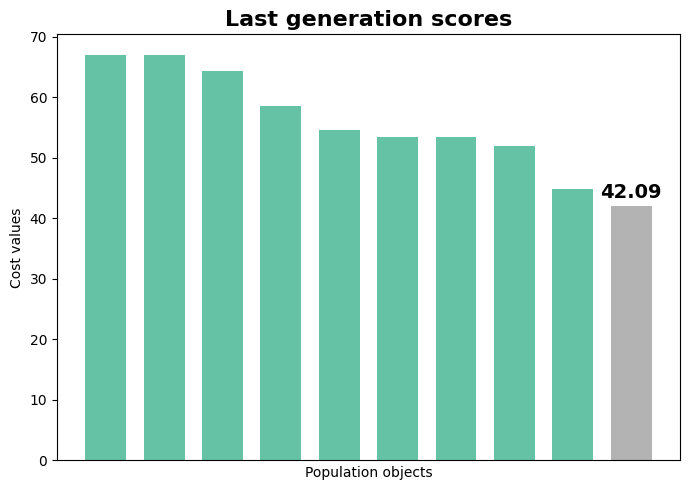
\includegraphics[scale = 0.75]{images/mutype_ubc_exp1_graphScore.png}
                \caption{Last Generation Scores (Tipo de Mutação = uniform\_by\_center - Experimento 1) }
            \end{figure}

            \textbf{Melhores indivíduos por geração}:\\
            
            [53.40877497913901,\\ 53.40877497913901,\\ 53.40877497913901,\\ 53.40877497913901,\\ 51.87570011121599,\\ 44.808756846535,\\ 44.808756846535,\\ 44.808756846535,\\ 42.08916277946018,\\ 42.08916277946018]

        \newpage
        \item Experimento 2:
            \begin{figure}[H]
                \centering
                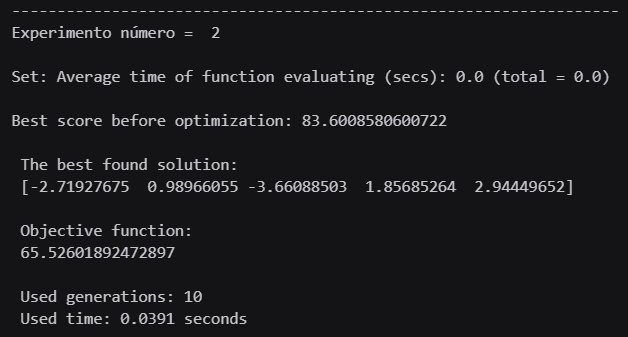
\includegraphics[scale = 0.75]{images/mutype_ubc_exp2.png}
                \caption{Tipo de Mutação = uniform\_by\_center - Experimento 2 }
            \end{figure}

            \begin{figure}[H]
                \centering
                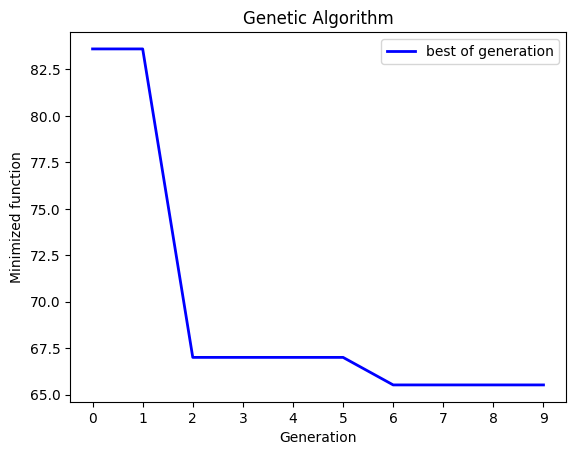
\includegraphics[scale = 0.75]{images/mutype_ubc_exp2_graphGA.png}
                \caption{Gráfico GA (CTipo de Mutação = uniform\_by\_center - Experimento 2) }
            \end{figure}

            \begin{figure}[H]
                \centering
                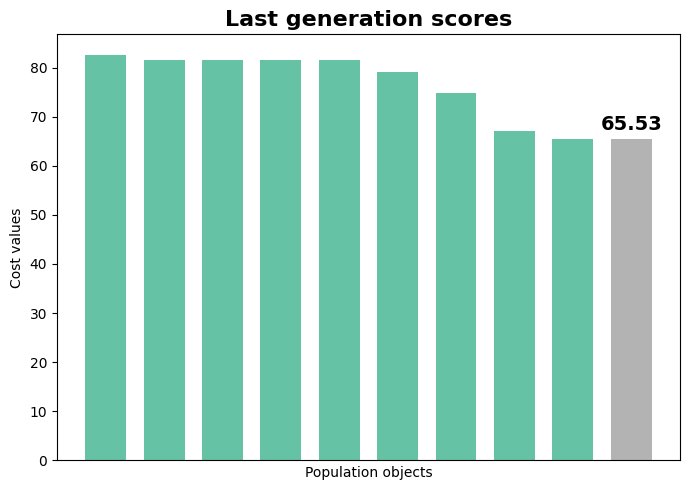
\includegraphics[scale = 0.75]{images/mutype_ubc_exp2_graphScore.png}
                \caption{Last Generation Scores (Tipo de Mutação = uniform\_by\_center - Experimento 2) }
            \end{figure}

            \textbf{Melhores indivíduos por geração}:\\
            
            [83.6008580600722,\\ 83.6008580600722,\\ 67.0073325501038,\\ 67.0073325501038,\\ 67.0073325501038,\\ 67.0073325501038,\\ 65.52601892472897,\\ 65.52601892472897,\\ 65.52601892472897,\\ 65.52601892472897] \\

            \textbf{Tipo de Mutação}: uniform by center,\\
            
            \textbf{Média dos Melhores por Geração}:\\
            
            [68.50481651960561,\\ 68.50481651960561,\\ 60.208053764621404,\\ 60.208053764621404,\\ 59.441516330659894,\\ 55.9080446983194,\\ 55.16738788563198,\\ 55.16738788563198,\\ 53.80759085209458,\\ 53.80759085209458]
    \end{itemize}
\end{itemize}



\begin{itemize}
    \item \textbf{Tipo de Mutação = gauss\_by\_center}:
    \begin{itemize}
        \item Experimento 1:
            \begin{figure}[H]
                \centering
                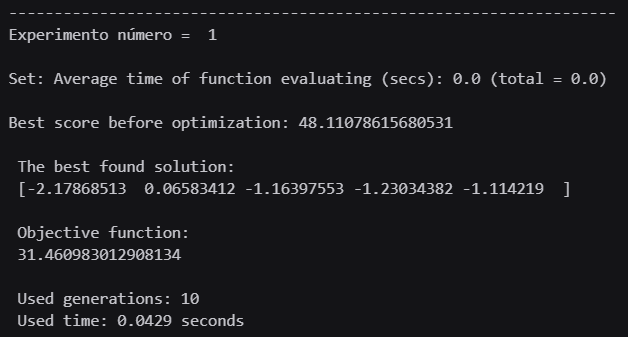
\includegraphics[scale = 0.75]{images/mutype_gbc_exp1.png}
                \caption{Tipo de Mutação = gauss\_by\_center - Experimento 1 }
            \end{figure}

            \begin{figure}[H]
                \centering
                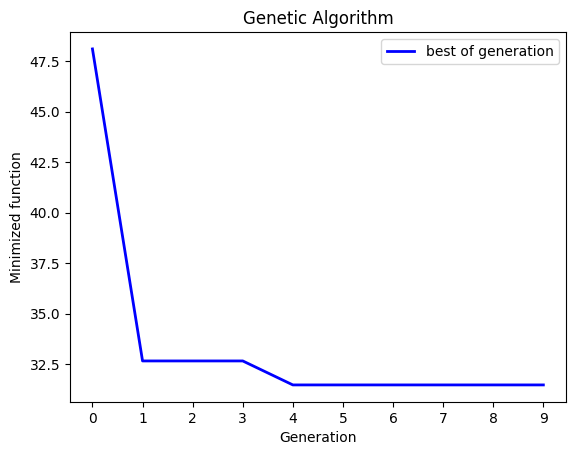
\includegraphics[scale = 0.75]{images/mutype_gbc_exp1_graphGA.png}
                \caption{Gráfico GA (CTipo de Mutação = gauss\_by\_center - Experimento 1) }
            \end{figure}

            \begin{figure}[H]
                \centering
                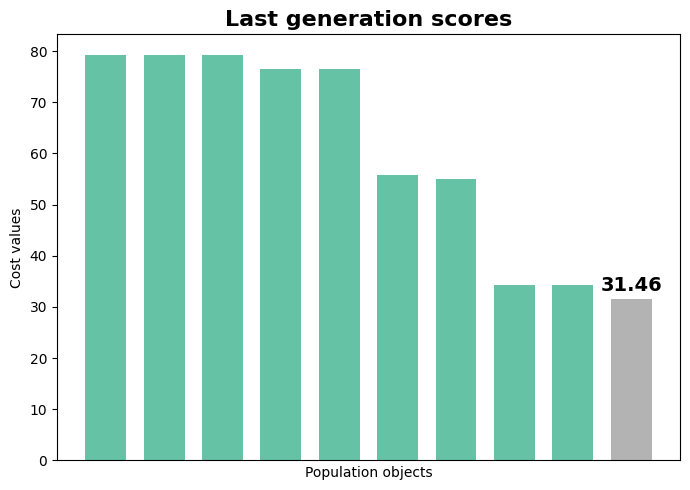
\includegraphics[scale = 0.75]{images/mutype_gbc_exp1_graphScore.png}
                \caption{Last Generation Scores (Tipo de Mutação = gauss\_by\_center - Experimento 1) }
            \end{figure}

            \textbf{Melhores indivíduos por geração}:\\
            
            [48.11078615680531,\\ 32.64927549631254,\\ 32.64927549631254,\\ 32.64927549631254,\\ 31.460983012908134,\\ 31.460983012908134,\\ 31.460983012908134,\\ 31.460983012908134,\\ 31.460983012908134,\\ 31.460983012908134]

        \newpage
        \item Experimento 2:
            \begin{figure}[H]
                \centering
                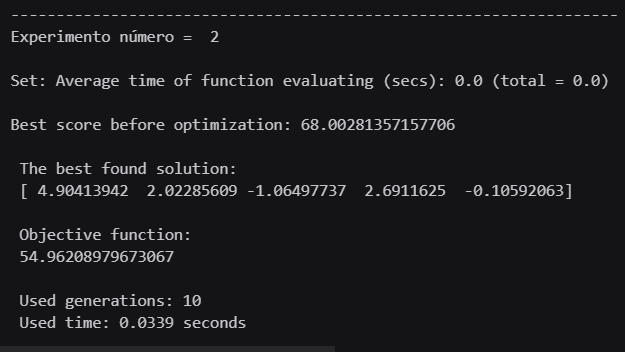
\includegraphics[scale = 0.75]{images/mutype_gbc_exp2.png}
                \caption{Tipo de Mutação = gauss\_by\_center - Experimento 2 }
            \end{figure}

            \begin{figure}[H]
                \centering
                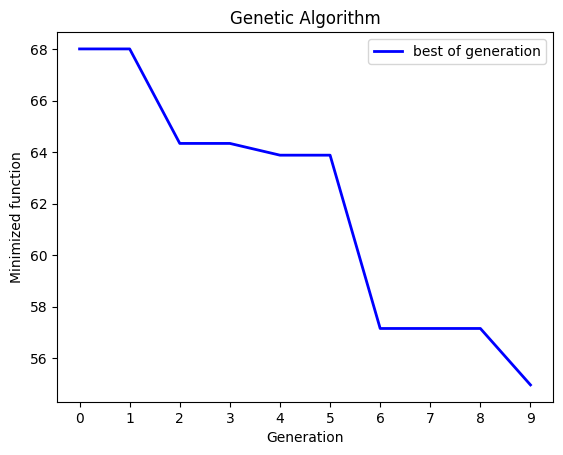
\includegraphics[scale = 0.75]{images/mutype_gbc_exp2_graphGA.png}
                \caption{Gráfico GA (CTipo de Mutação = gauss\_by\_center - Experimento 2) }
            \end{figure}

            \begin{figure}[H]
                \centering
                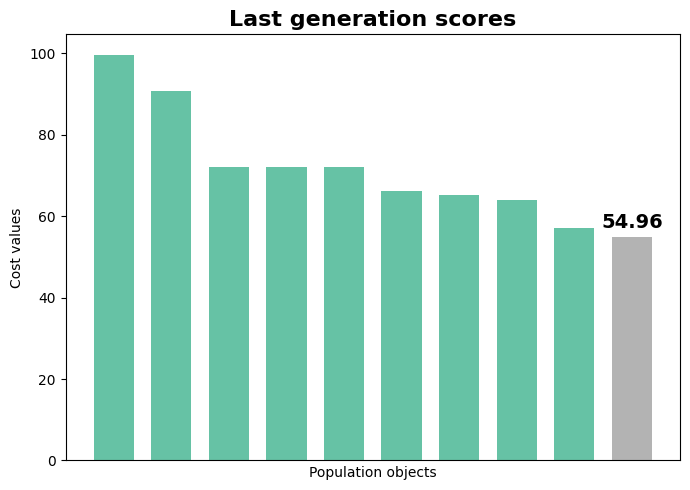
\includegraphics[scale = 0.75]{images/mutype_gbc_exp2_graphScore.png}
                \caption{Last Generation Scores (Tipo de Mutação = gauss\_by\_center - Experimento 2) }
            \end{figure}

            \textbf{Melhores indivíduos por geração}:\\
            
            [68.00281357157706,\\ 68.00281357157706,\\ 64.33507128746555,\\ 64.33507128746555,\\ 63.87892878802599,\\ 63.87892878802599,\\ 57.1527018417801,\\ 57.1527018417801,\\ 57.1527018417801,\\ 54.96208979673067] \\

            \textbf{Tipo de Mutação}: gauss by center,\\
            
            \textbf{Média dos Melhores por Geração}:\\
            
            [58.05679986419119,\\ 50.3260445339448,\\ 48.49217339188905,\\ 48.49217339188905,\\ 47.66995590046706,\\ 47.66995590046706,\\ 44.306842427344115,\\ 44.306842427344115,\\ 44.306842427344115,\\ 43.211536404819405]
    \end{itemize}
\end{itemize}


\textbf{Interpretação dos Resultados}:\\

\begin{figure}[H]
    \centering
    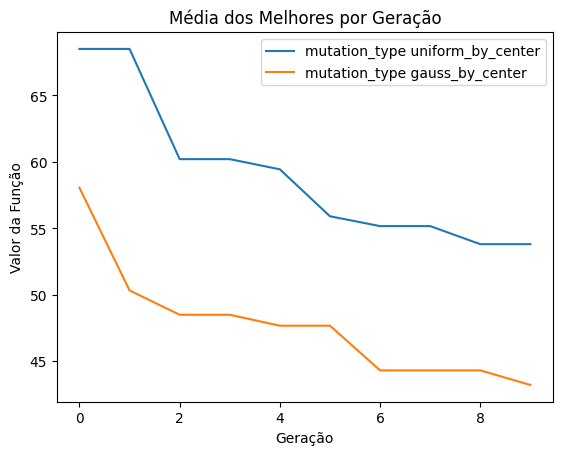
\includegraphics[scale = 0.75]{images/mutype_ubc_graph_media.png}
    \caption{Gráfico comparativo - Tipo de Mutação }
\end{figure}

\begin{figure}[H]
    \centering
    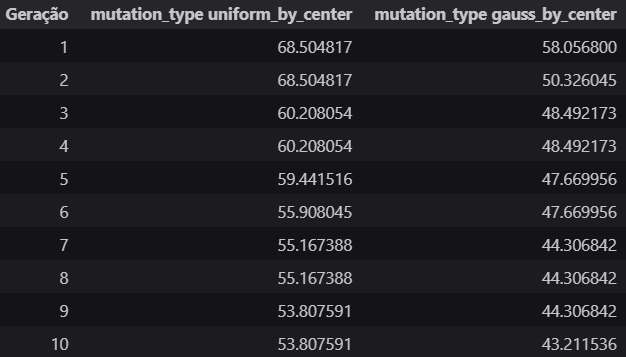
\includegraphics[scale = 0.90]{images/mutype_ubc_tabela_comparativa.png}
    \caption{Tabela comparativa - Tipo de Mutação - média dos melhores }
\end{figure}

\begin{enumerate}
    \item \textbf{mutation\_type = uniform\_by\_center}:
    \begin{itemize}
        \item A função objetivo melhora de forma mais gradual.
        \item Resulta em menor diversidade genética, limitando a exploração.
        \item Adequado para cenários onde a estabilidade e uma convergência mais controlada são preferidas. Tem convergência mais lenta, mas permite encontrar soluções melhores ao longo do tempo.
    \end{itemize}
    \item \textbf{mutation\_type = gauss\_by\_center}:
    \begin{itemize}
        \item  A função objetivo melhora rapidamente nas primeiras gerações, indicando uma rápida convergência inicial.
        \item Permite maior diversidade genética, ajudando a explorar melhor o espaço de soluções e evitando a convergência prematura.
        \item Melhor para explorar o espaço de soluções de forma mais agressiva, encontrando soluções de alta qualidade rapidamente. Convergência rápida, com resultados finais melhores.
    \end{itemize}
\end{enumerate}





\newpage
\subsubsection{Alternando o tipo de seleção (selection\_type)}


\begin{itemize}
    \item \textbf{Tipo de Seleção = Roleta}:
    \begin{itemize}
        \item Experimento 1:
            \begin{figure}[H]
                \centering
                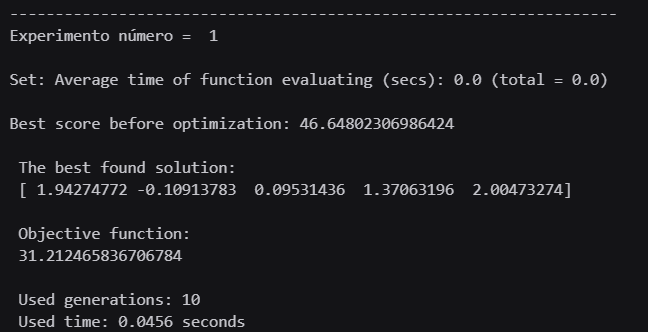
\includegraphics[scale = 0.75]{images/roulette_exp1.png}
                \caption{Tipo de Seleção = Roleta - Experimento 1 }
            \end{figure}

            \begin{figure}[H]
                \centering
                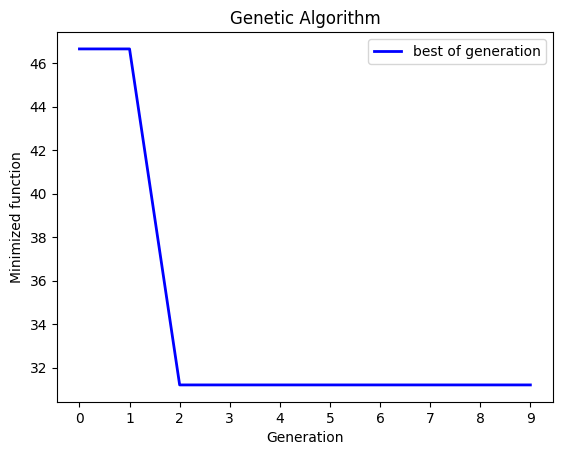
\includegraphics[scale = 0.75]{images/roulette_exp1_graphGA.png}
                \caption{Gráfico GA (Tipo de Seleção = Roleta - Experimento 1) }
            \end{figure}

            \begin{figure}[H]
                \centering
                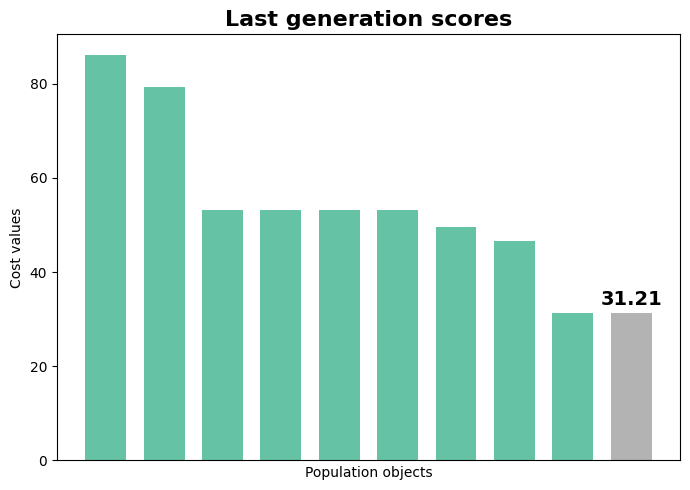
\includegraphics[scale = 0.75]{images/roulette_exp1_graphScore.png}
                \caption{Last Generation Scores (Tipo de Seleção = Roleta - Experimento 1) }
            \end{figure}

            \textbf{Melhores indivíduos por geração}:\\
            
            [46.64802306986424,\\ 46.64802306986424,\\ 31.212465836706784,\\ 31.212465836706784,\\ 31.212465836706784,\\ 31.212465836706784,\\ 31.212465836706784,\\ 31.212465836706784,\\ 31.212465836706784,\\ 31.212465836706784]

        \newpage
        \item Experimento 2:
            \begin{figure}[H]
                \centering
                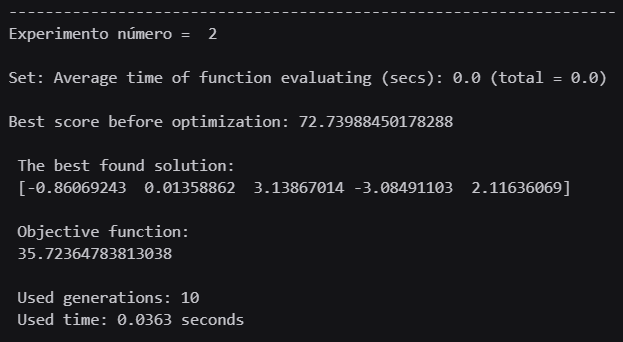
\includegraphics[scale = 0.75]{images/roulette_exp2.png}
                \caption{Tipo de Seleção = Roleta - Experimento 2 }
            \end{figure}

            \begin{figure}[H]
                \centering
                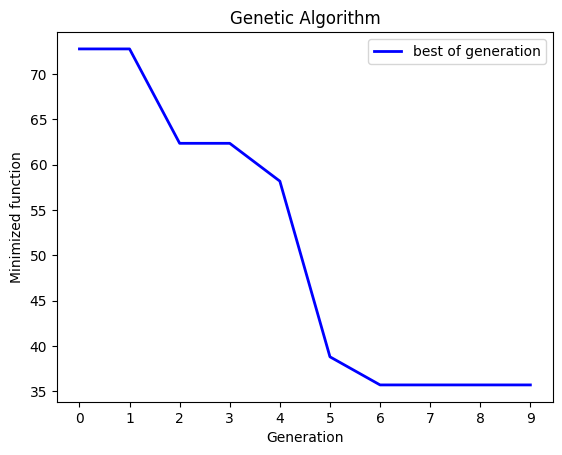
\includegraphics[scale = 0.75]{images/roulette_exp2_graphGA.png}
                \caption{Gráfico GA (Tipo de Seleção = Roleta - Experimento 2) }
            \end{figure}

            \begin{figure}[H]
                \centering
                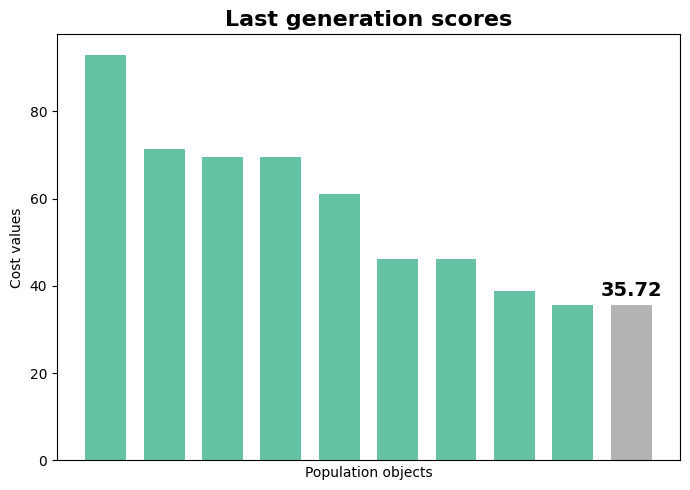
\includegraphics[scale = 0.75]{images/roulette_exp2_graphScore.png}
                \caption{Last Generation Scores (Tipo de Seleção = Roleta - Experimento 2) }
            \end{figure}

            \textbf{Melhores indivíduos por geração}:\\
            
            [72.73988450178288,\\ 72.73988450178288,\\ 62.34085904353354,\\ 62.34085904353354,\\ 58.17095245340959,\\ 38.82051406230397,\\ 35.72364783813038,\\ 35.72364783813038,\\ 35.72364783813038,\\ 35.72364783813038] \\

            \textbf{Tipo de Seleção}: Roleta,\\
            
            \textbf{Média dos Melhores por Geração}:\\
            
            [59.69395378582356,\\ 59.69395378582356,\\ 46.77666244012016,\\ 46.77666244012016,\\ 44.691709145058184,\\ 35.01648994950538,\\ 33.46805683741859,\\ 33.46805683741859,\\ 33.46805683741859,\\ 33.46805683741859]
    \end{itemize}
\end{itemize}


\begin{itemize}
    \item \textbf{Tipo de Seleção = Torneio}:
    \begin{itemize}
        \item Experimento 1:
            \begin{figure}[H]
                \centering
                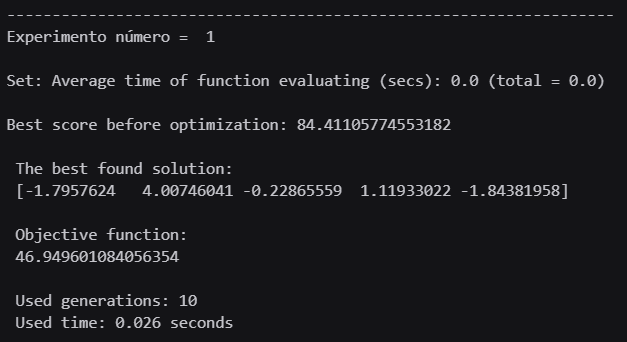
\includegraphics[scale = 0.75]{images/tournament_exp1.png}
                \caption{Tipo de Seleção = Torneio - Experimento 1 }
            \end{figure}

            \begin{figure}[H]
                \centering
                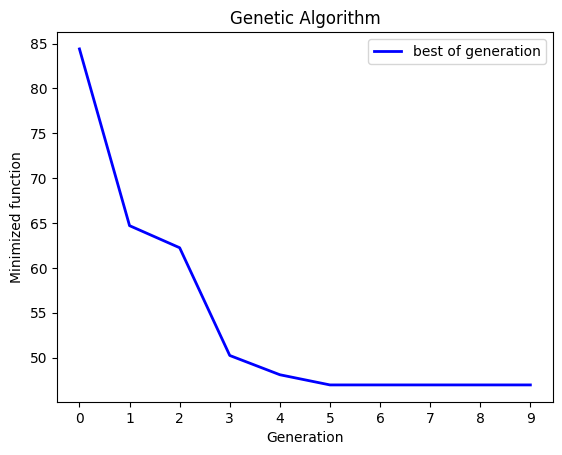
\includegraphics[scale = 0.75]{images/tournament_exp1_graphGA.png}
                \caption{Gráfico GA (Tipo de Seleção = Torneio - Experimento 1) }
            \end{figure}

            \begin{figure}[H]
                \centering
                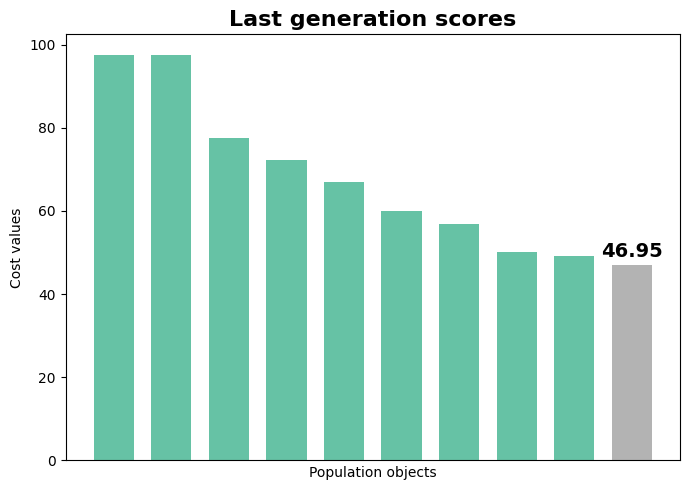
\includegraphics[scale = 0.75]{images/tournament_exp1_graphScore.png}
                \caption{Last Generation Scores (Tipo de Seleção = Torneio - Experimento 1) }
            \end{figure}

            \textbf{Melhores indivíduos por geração}:\\
            
            [84.41105774553182,\\ 64.70557521923004,\\ 62.24374536006444,\\ 50.232085730819065,\\ 48.08477665929036,\\ 46.949601084056354,\\ 46.949601084056354,\\ 46.949601084056354,\\ 46.949601084056354,\\ 46.949601084056354]

        \newpage
        \item Experimento 2:
            \begin{figure}[H]
                \centering
                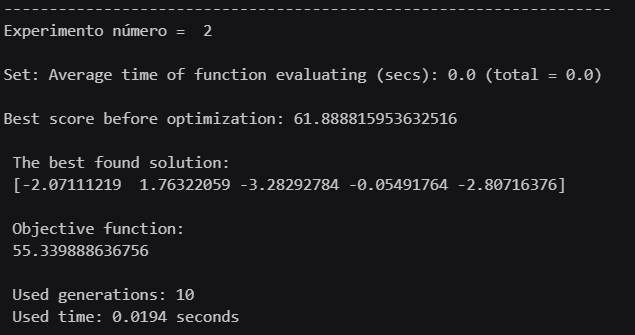
\includegraphics[scale = 0.75]{images/tournament_exp2.png}
                \caption{Tipo de Seleção = Torneio - Experimento 2 }
            \end{figure}

            \begin{figure}[H]
                \centering
                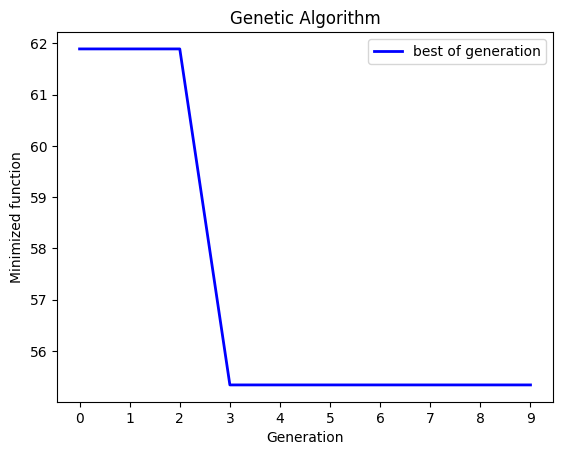
\includegraphics[scale = 0.75]{images/tournament_exp2_graphGA.png}
                \caption{Gráfico GA (Tipo de Seleção = Torneio - Experimento 2) }
            \end{figure}

            \begin{figure}[H]
                \centering
                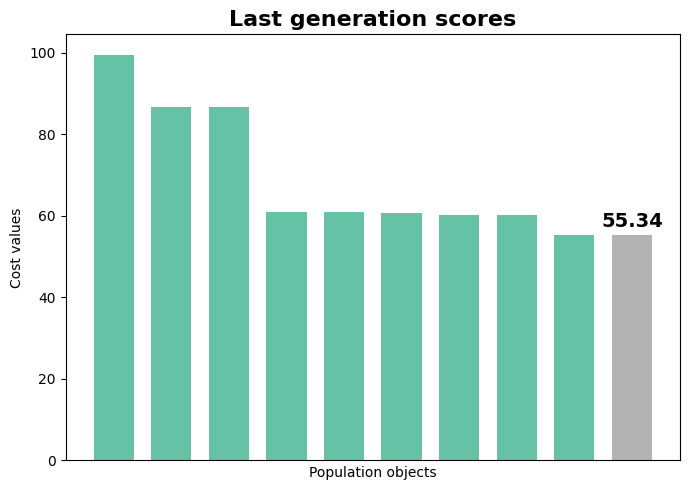
\includegraphics[scale = 0.75]{images/tournament_exp2_graphScore.png}
                \caption{Last Generation Scores (Tipo de Seleção = Torneio - Experimento 2) }
            \end{figure}

            \textbf{Melhores indivíduos por geração}:\\
            
            [61.888815953632516,\\ 61.888815953632516,\\ 61.888815953632516,\\ 55.339888636756,\\ 55.339888636756,\\ 55.339888636756,\\ 55.339888636756,\\ 55.339888636756,\\ 55.339888636756,\\ 55.339888636756] \\

            \textbf{Tipo de Seleção}: Torneio,\\
            
            \textbf{Média dos Melhores por Geração}:\\
            
            [73.14993684958216,\\ 63.29719558643128,\\ 62.06628065684848,\\ 52.78598718378753,\\ 51.71233264802318,\\ 51.14474486040618,\\ 51.14474486040618,\\ 51.14474486040618,\\ 51.14474486040618,\\ 51.14474486040618]
    \end{itemize}
\end{itemize}



\textbf{Interpretação dos Resultados}:\\

\begin{figure}[H]
    \centering
    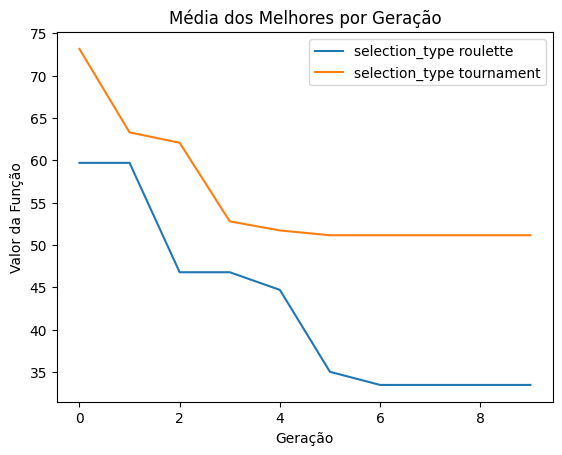
\includegraphics[scale = 0.75]{images/selectype_graph_media.png}
    \caption{Gráfico comparativo - Tipo de Seleção }
\end{figure}

\begin{figure}[H]
    \centering
    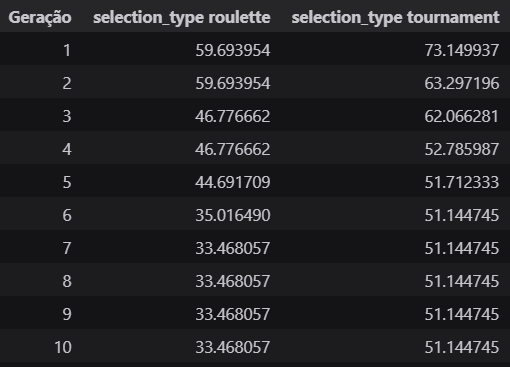
\includegraphics[scale = 0.90]{images/selectype_tabela_comparativa.png}
    \caption{Tabela comparativa - Tipo de Seleção - média dos melhores }
\end{figure}

\begin{enumerate}
    \item \textbf{Tipo de seleção = roleta}:
    \begin{itemize}
        \item A função objetivo melhora de forma mais gradual.
        \item Resulta em menor diversidade genética, limitando a exploração.
        \item Adequado para cenários onde a estabilidade e uma convergência mais controlada são preferidas. Tem convergência mais lenta, mas permite encontrar soluções melhores ao longo do tempo.
    \end{itemize}
    \item \textbf{Tipo de seleção = torneio}:
    \begin{itemize}
        \item  A função objetivo melhora rapidamente nas primeiras gerações, indicando uma rápida convergência inicial.
        \item Permite maior diversidade genética, ajudando a explorar melhor o espaço de soluções e evitando a convergência prematura.
        \item Melhor para explorar o espaço de soluções de forma mais agressiva, encontrando soluções de alta qualidade rapidamente. Convergência rápida, com resultados finais melhores.
    \end{itemize}
\end{enumerate}


\section{Conclusão}

Com base nas análises realizadas dos diversos parâmetros do Algoritmo Genético, podemos fazer as seguintes inferências e conclusões sobre a configuração ideal para encontrar a função de mínimo para o problema no menor tempo possível, ou seja, com a menor quantidade de gerações:\\

\textbf{Parâmetros Testados}\\

\begin{enumerate}
    \item \textbf{Número de Gerações (max\_num\_iteration)}:

Testamos os valores de 10, 20 e 50 iterações. Observou-se que o aumento do número de iterações melhora a precisão da solução encontrada, mas também aumenta o tempo de execução. Para um bom equilíbrio entre precisão e tempo, 20 iterações mostraram-se suficientes na maioria dos casos.


    \item \textbf{Tamanho da População (population\_size)}:

Testamos os valores de 5 e 20. Observamos que uma população maior melhora a diversidade genética e a qualidade das soluções encontradas, mas aumenta o tempo de cada iteração. Um tamanho de 10 a 20 é um bom compromisso.

\item \textbf{Probabilidade de Mutação (mutation\_probability)}:

Testamos valores de 0.001, 0.01 e 0.1. Uma taxa de mutação de 0.01 proporcionou um bom equilíbrio entre exploração e convergência, evitando a convergência prematura e mantendo a diversidade.


\item \textbf{Razão de Elitismo (elit\_ratio)}:

Testamos valores de 0.2 e 0.8. Um valor mais baixo (0.2) proporcionou melhores resultados, permitindo que o algoritmo mantenha a diversidade genética e evite a convergência prematura.

\item \textbf{Probabilidade de Crossover (crossover\_probability)}:

Testamos valores de 0.1 e 0.6. A probabilidade de 0.6 permitiu uma melhor troca de material genético entre os indivíduos, resultando em uma convergência mais eficiente.


\item \textbf{Porção dos Pais (parents\_portion)}:

Testamos valores de 0.2 e 0.8. A porção de 0.8 proporcionou uma boa exploração do espaço de busca, permitindo que mais soluções potenciais fossem exploradas.


\item \textbf{Tipos de Crossover (crossover\_type)}:

Testamos 'one\_point' e 'two\_point'. O 'two\_point' proporcionou uma melhor convergência inicial, mas ambos os métodos são eficazes.


\item \textbf{Tipos de Mutação (mutation\_type)}:

Testamos 'uniform\_by\_center' e 'gauss\_by\_center'. A mutação Gaussiana mostrou-se mais eficaz em manter a diversidade genética e proporcionar melhores soluções finais.

\item \textbf{Tipos de Seleção (selection\_type)}:

Testamos 'roulette' e 'tournament'. A seleção por torneio mostrou-se mais eficiente em encontrar boas soluções rapidamente, mas a roleta proporcionou uma melhor diversidade genética.

\end{enumerate}

\textbf{Configuração Recomendada}\\

Com base nas análises, a seguinte configuração seria recomendada para alcançar a função de mínimo com a menor quantidade de gerações e tempo possível: \\

\begin{itemize}
    \item Número de Gerações: \textbf{20}
    \item Tamanho da População: \textbf{20}
    \item Probabilidade de Mutação: \textbf{0.01}
    \item Razão de Elitismo: \textbf{0.2}
    \item Probabilidade de Crossover: \textbf{0.6}
    \item Porção dos Pais: \textbf{0.8}
    \item Tipo de Crossover: \textbf{two\_point}
    \item Tipo de Mutação: \textbf{gauss\_by\_center}
    \item Tipo de Seleção: \textbf{tournament}
\end{itemize}


Para testar os parâmetros recomendados dentro deste contexto, executamos um novo teste inserindo-os no dicionário. Obtivemos o seguinte resultado:


\begin{figure}[H]
    \centering
    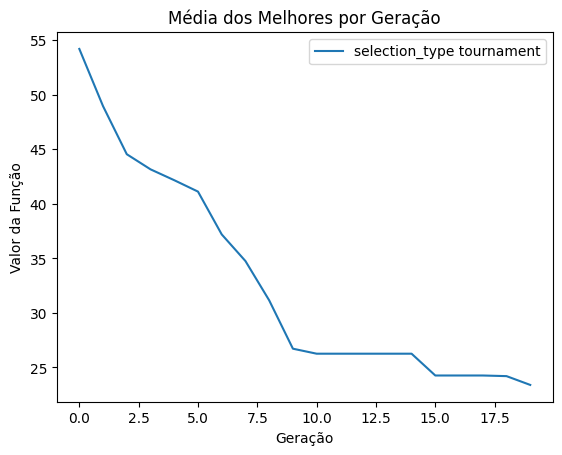
\includegraphics[scale = 0.75]{images/final.png}
    \caption{Gráfico da média dos melhores por geração - Teste final}
\end{figure}

Com base nas análises e nos resultados obtidos, podemos concluir que a configuração final escolhida proporcionou uma boa eficiência do Algoritmo Genético para encontrar a função de mínimo para o problema em um tempo razoável. O resultado mostra que a função objetivo esteve mais próximo de alcançar o mínimo em todas as execuções, demonstrando a eficácia dos parâmetros escolhidos.\\

No entanto, é sempre válido ajustar os parâmetros conforme necessário para atender às especificidades de cada problema.










% REFERENCIAS %%%%%%%%%%%%%%%%%%%%%%%%%%%%%%%%%%%%%%%%%%%%%%%%%%%%%%%%%%%%%%



\end{document}